\documentclass[12pt, a4paper, twoside, openright, final]{book}
% ! RECORDAR PONER EL TÍTULO DE LA TÉSIS ANTES DE IMPRIMIR EL ARCHIVO (EN PORTADA, Y EN FOOTNOTE GENERAL)
% * sudo tlmgr install <package>
% ================================================================================================================================
% Preámbulo
% ================================================================================================================================
\usepackage{preamble}
% ================================================================================================================================
% Documento
% ================================================================================================================================
\begin{document}
% ================================================================================================================================
% Portada y Front Matter
% ================================================================================================================================
\begin{titlepage}
    \begin{center}
        \vspace*{1cm}
        
        \Huge
        \textbf{Distribución de la presión dentro de los nucleones en un modelo de bolsa de Tsallis-MIT}
        
        \vspace{0.5cm}
        \LARGE
        Física de partículas
        
        \vspace{1.5cm}
        
        Presenta: \textbf{Manuel Alejandro Matías Astorga} \\
        Director de tésis: \textbf{Dr. Gerardo Herrera Corral}
        
        \vfill
        
        A thesis presented for the degree of\\
        Doctor of Philosophy
        
        \vspace{0.8cm}
        
        
\includegraphics[width=0.3\textwidth]{Cinvestav-logo}
        
        \Large
        Departamento de física\\
        CINVESTAV\\
        CDMX, México\\
        \today
        
    \end{center}
\end{titlepage}

\newpage
\thispagestyle{empty}

\frontmatter


% Abstract en español e inglés
\chapter*{Abstract}
\addcontentsline{toc}{chapter}{Resumen}
\label{ch: abstract}
\abstractsection{spanish}{
    \begin{flushright}
        Resumen en español
    \end{flushright}
    }
\abstractsection{english}{
    \begin{flushright}
        This is the abstract
    \end{flushright}
    }

\newpage
\thispagestyle{empty}

% Agradecimientos
\chapter*{Agradecimientos}
\addcontentsline{toc}{chapter}{Agradecimientos}
\label{ch: Agradecimientos}
\begin{flushright}
CONAHCYT, CINVESTAV, Dr Gerardo H. C.

Agradezco y acredito a \href{https://www.overleaf.com/learn/latex/How_to_Write_a_Thesis_in_LaTeX_(Part_1)%3A_Basic_Structure}{Josh Cassidy} por la plantilla de la portada de mi tésis.
\end{flushright}

\newpage
\thispagestyle{empty}

% Índices
\renewcommand{\contentsname}{Contenido}
\tableofcontents % Podríamos usar \usepackage{tocloft} para personalizar el ToC
\renewcommand{\listfigurename}{Lista de figuras}
\listoffigures

\newpage
\thispagestyle{empty}
\renewcommand{\listtablename}{Lista de Tablas}
\listoftables

\newpage
\thispagestyle{empty}

% ================================================================================================================================
% Main Matter
% ================================================================================================================================
\mainmatter

\renewcommand{\chaptername}{Capítulo}

\chapter*{Introducción}
\addcontentsline{toc}{chapter}{Introducción}

% =====================Estilo de página================================
\pagestyle{fancy}
\fancyhf{} % clear all header fields
\fancyhead[LE]{\nouppercase{\textbf{Introducción} \hfill}}
\fancyhead[RO]{\nouppercase{\hfill \textbf{Introducción}}}
\fancyfoot[LE]{\nouppercase{\thepage \hfill \emph{Thesis title}}}
\fancyfoot[RO]{\nouppercase{\emph{Thesis title} \hfill \thepage}}
% =====================================================================

% 12 345.678 90                     \num{12345,67890} \\
% 0.3 ×1045                         \num{.3e45} \\
% 1 ±2i                             \complexnum{1+-2i}
% 1.654 ×2.34 ×3.430                \numproduct{1.654 x 2.34 x 3.430}
% kg m s−1                          \unit{kg.m.s^{-1}}
% kg m s−1                          \unit{\kilogram\metre\per\second} 
% kg m/s                            \unit[per-mode = symbol]{\kilogram\metre\per\second}
% kg m/(A s)                        \unit[per-mode = symbol]{\kilogram\metre\per\ampere\per\second}
% 

De acuerdo con el modelo de \acrfull{qcd} las partículas hadrónicas están formadas de quarks los cuales se encuentran confinados dentro de la dichos hadrones \Gls{maths}.

% Renombrando las figuras
\renewcommand{\figurename}{Fig.}

\begin{wrapfigure}{r}{0.45\textwidth}
\centering
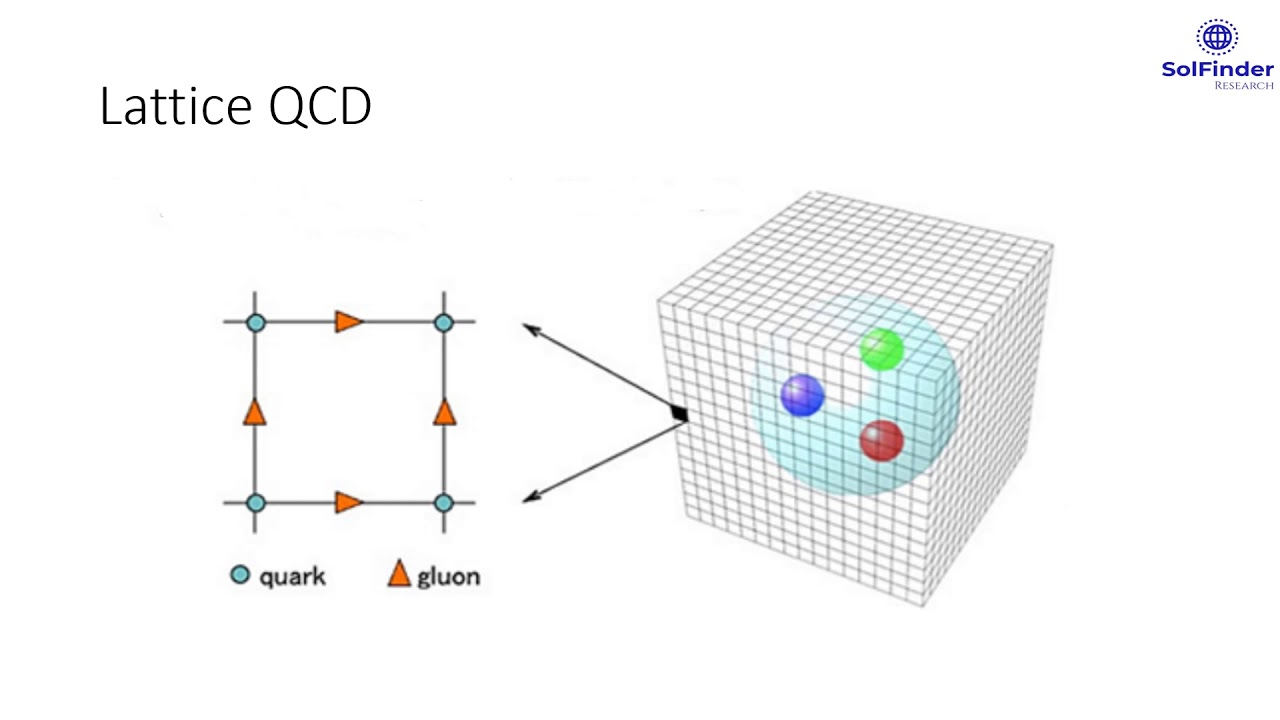
\includegraphics[width=0.4\textwidth]{./Images/LQCD.jpg}
\caption[Red LQCD]{\emph{Diagrama de red tipo LQCD en donde los nodos se encuentran donde los quarks y las aristas representan campos gluónicos}}
\label{fig: LQCD}
\end{wrapfigure}

%Over the years, various phenomenological descriptions of proton structures have been proposed, such as string models [1,2], which depict hadrons as oscillating strings; bag models, which consider quarks confined within a cavity; and valon models
Por años, varias descripciones fenomenológicas de las estructuras del protón han sido propuestas, tales como modelos de cuerdas \cite{Artru1974, Andersson_1983} \cite{Artru1974, Andersson_1983}, que describe hadrones como cuerdas oscilantes, modelos de bolsa \cite{AIHPA_1968__8_2_163_0,DeTar_1983}, que considera quarks confinados en una cavidad, y modelos de valones \cite{Hwa_1981}.

Con el fin de explorar la física de materia quark, se han desarrollado varias técnicas que permiten vislumbrar los efectos de ese tipo de interacciones como por ejemplo \acrfull{lqcd}; y por otro lado, se han desarrollado modelos que pueden bosquejar este tipo de interacciones a partir de simplificaciones como sucede en el modelo de bolsa (\acrfull{bm}), el modelo de cuerdas, el modelo de partones y un largo etcétera\cite{DeTar_1983}, puesto que ocurren interacciones no lineales dentro de los hadrones. 

%Lattice QCD computations provide reliable results of hadron structures that con- tain heavy quarks and have recently been used as state-of-the-art calculations by the HAL-QCD collaboration[6,7]. The description obtained by HAL QCD of the final state strong interactions between proton–neutron and proton–hyperons systems was compared to the experimental results published by the ALICE Collaboration 

Cálculos de \acrshort{lqcd} proporcionan resultados confiables de estructuras hadrónicas que contienen quarks pesados y ha sido recientemente usadas como cálculos de estado de arte por la colaboración HAL-QCD \cite{Iritani_2019,Hatsuda_2017}. La descripción obtenida por HAL QCD de los estados finales de interacciones fuertes entre sistemas protón-neutrón y protón hiperones fue comparado a los resultados experimentales publicados por la colaboración ALICE \cite{Collaboration2020, Collaboration2021}

\qty{10}{cm}

\num{1.2304} \unit{\candela}

\acrshort{lqcd} consiste en una técnica numérica que lleva a cabo gran cantidad de cálculos en una red espacio - temporal Euclídea muy grande (los parámetros de red $a$ son del orden de $\mathit{\unit{\femto\meter}}$ o como se menciona en [INTRO A LQCD], en un rango de $2 \, \unit{GeV} \leq {a}^{-1} \leq 5 \, \unit{GeV}$), Fig.~\ref{fig: LQCD}. Debido a que ocupa redes con millones de nodos, la dificultad de este tipo de modelos recae en la cantidad de cálculos necesarios para resolver dichos modelos. 
Partiendo de esto, se tiene un nuevo problema: \emph{el problema del signo} [más referencias], el cual surge en simulaciones Monte Carlo como las que se ocupan para resolver \acrshort{lqcd}, esto consiste en que el peso de las configuraciones de simulaciones cuánticas Monte Carlo se vuelven negativas o incluso complejas, y por lo tanto, no pueden ser interpretadas como proabilidades clásicas[Sign problem in QMC simulation]. 

NOTA: Hablar acerca del operador de Dirac no hermitiano

Los cálculos de \acrshort{lqcd} 

han conseguido resultados fiables acerca de las estructuras de hadrones que contienen quarks pesados


NOTA: Hablar acerca de resultados obtenidos con LQCD

Hemos propuesto un modelo que se basa en el modelo de bolsa (\acrshort{bm}) del \acrfull{mit} [add ref] y estadística no extensiva de Tsallis. Para simplificarlo lo llamaremos \acrshort{t-mitbm}. Por un lado hemos considerado el marco teórico del modelo de bolsa el cual consiste en que los hadrones son considerados como recipientes cerrados en donde se hallan un mar de quarks y gluones que interaccionan y están encerrados dentro del los límites del hadrón que es la bolsa por una presión dirigida hacia adentro que contrarresta los efectos de la presión debida a los quarks, los gluones y su fuerza de interacción (figura \ref{fig: Bolsa}) [referencias al modelo de bolsa]. 

\begin{wrapfigure}{l}{0.4\textwidth}
\centering
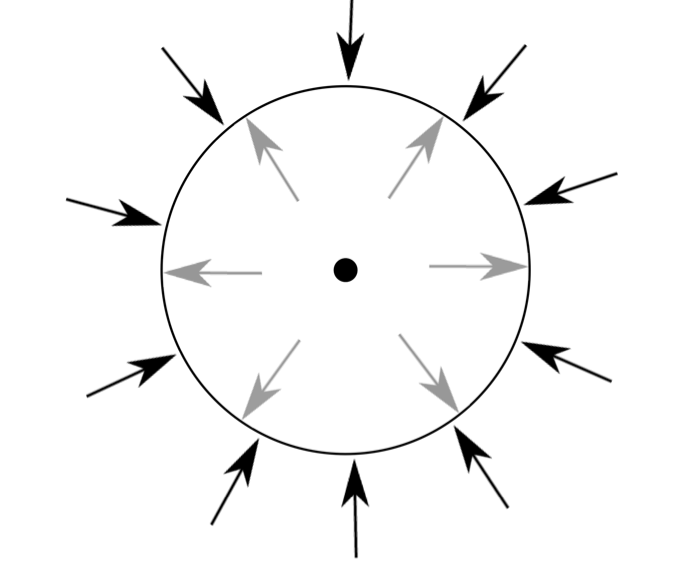
\includegraphics[width=0.4\textwidth]{./Images/Bag model.png}
\caption[Diagrama de bolsa]{\emph{Diagrama de bolsa, en el interior de la bolsa tenemos la presión generada por un plasma de quarks y gluones que considera tanto la presión dada por los quarks, por los gluones y por la interacción entre estos (dentro) y por otro lado la presión hacia el interior dada por la bolsa que coincide con los límites del hadrón.}}
\label{fig: Bolsa}
\end{wrapfigure}

De esta manera, en nuestro modelo consideramos una simplificación de todos los cálculos que se ocupan en \acrshort{qcd}, con el fin de reducir esas interacciones a la contribución de una presión de bolsa $B$.

Como en el código de \ref{code:python_example}

Por otro lado, consideramos la estadística no extensiva de Tsallis ya que proporciona el modelo necesario para representar al plasma de quarks y gluones (visto como gases de Fermi y Dirac por simplificación) con un parámetro que considera la interacción entre los quarks y los gluones. Este modelo se ha escogido por sus varias aplicaciones en otras áreas de investigación [más referencias] y que se ajusta muy bien a este modelo por tratarse de partículas que interaccionan y con ello simplifican la no linearidad propia de esto [más referencias]. Cabe mencionar, que en este marco se pueden considerar gases con potencial químico, $\mu$, no nulo lo cual es una ventaja a la hora de estudiar los diversos escenarios en los que los hadrones se encuentran.

%Here, we propose a phenomenological description based on the MIT bag model [10,11] and a non-extensive statistical approach. This could be referred to as the T-MIT bag model to abbreviate the merger of Tsallis non-extensive statistics and the MIT Bag Model [12].

Aquí proponemos una descripción fenomenológica basada en el modelo de bolsa del MIT \cite{Chodos_1974,Chodos1974a} y una aproximación estadística no extensiva. Esta podría ser referida como \acrshort{t-mitbm} para abreviar la unión de la estadística no extensiva de Tsallis y el \acrshort{mit} \acrshort{bm} \cite{Barboza_Mendoza_2019}

De esta manera, el modelo \acrshort{t-mitbm} es un modelo que introduce un potencial químico, $\mu$, distinto de cero para estudiar el modelo hadrónico un poco más extendido. Hemos comparado estos resultados con los obtenidos en [Nature], donde se ha obtenido la distribución de presión de quarks dentro del protón usando \acrfull{dvcs}, lo cual consiste en dispersar fotones virtuales de altas energías radiadas por electrones y la emisión subsecuente de un protón real. El fotón en el estado final permite la estimación de transferencia de momento al protón, que permanece intacto. El análisis recae en métodos desarrollados para extraer información a partir de \acrfull{gpd} y \acrfull{cff}. Así se obtuvo una presión repulsiva de los quarks cerca del centro del protón y una presión de atadura a distancias por encima de $0.6 \, \mathit{\unit{\femto\meter}}$ del centro. Sin embargo, hay que recordar que esto solo corresponde a los quarks, la presión debido a los gluones no se considera.

NOTA: Agregar referecnias respecto a resultados experimentales acerca de la presión dentro del protón y la estructura del hadron.

%Tsallis statistics was introduced as a generalization of the Boltzmann–Gibbs statistics approach [13–17]. The Tsallis statistic has been widely used in high-energy physics. It was introduced for the first time to describe particle production in electron–positron collisions. The differential distributions of transverse momenta for charged hadrons with respect to the jet axis at several center-of-mass energies were successfully adjusted with a Tsallis function [18,19]. Tsallis distributions have also been used in proton–proton [20–23] and heavy ion [24,25] collisions to describe the experimental data. The observed success in describing the experimental data indicates that some underlying physics may be at work at a more fundamental level.

La estadística de Tsallis fue introducida como una generalización de la aproximación de \acrshort{bg} \cite{Tsallis1988,Beck_2003,Tsallis2009,Tsallis_2014,Tsallis_2009}. La estadística de Tsallis ha sido ampliamente usada en física de altas energías. Fue introducida por primera vez para describir producción de partículas en colisiones electrón positrón. Las distribuciones diferenciales de momento transversal para hadrones cargados con respecto al eje de jet en varias energías de centro de masa fueron ajustadas existosamente con una función de Tsallis \cite{Bediaga_2000,Collaboration1984}. Las distribuciones de Tsallis también han sido usadas en colisiones protón protón\cite{PhysRevLett.105.022002,Marques_2015,Bhattacharyya_2018,Khuntia_2017} y iones pesados \cite{Saraswat_2018,Saraswat_2017}
 para describir los datos experimentales.

%Here, we incorporate the non-extensive Tsallis statistics in the MIT bag model to describe fermions and bosons as non-independent components of hadrons. In the new T-MIT bag model, one can estimate the total pressure distribution inside nucleons. We compared the resulting profile with the extracted pressure distribution of quarks published recently [26].

Aquí, incorporamos la estadística no extensiva de Tsallis en el \acrshort{t-mitbm} para describir fermiones y bosones como componentes no independientes de los hadrones. En el nuevo \acrshort{t-mitbm}, uno puede estimar la distribución de presión total dentro de los nucleones. Comparamos el perfil resultante con la distribución de presión extraida de quarks publicada recientemente \cite{Burkert_2018}.

%On the experimental side, projects are now implementing techniques to gain more insight into the hadron structure [27], as well as the residual effects of strong nucleon- nucleon and nucleon–hyperon interactions [28,29]. The Electron Ion Collider (EIC) [30] planned for construction at Brookhaven National Laboratory will be dedicated to unrav- elling details of the strong interaction. It probes the transition between the perturbative and non-perturbative phenomena of QCD and the internal structure of protons and atomic nuclei. The EIC will reveal features of the sea of quark-antiquark pairs and key aspects of the gluon distribution. Effective models will continue to provide guidelines. The model proposed here offers a new approach to look at the structure of hadrons. We are not aware of similar advances aimed at estimating the pressure inside hadrons, although the fusion of the MIT bag model and Tsallis statistics has been performed previously [31,32].

Por el lado experimental, los proyectos están ahora implementando técnicas para ganar más conocimiento en la estructura del hadrón\cite{PhysRevLett.100.162002} así como los efectos residuales de interacciones fuertes nucleon nucleon y nucleon hiperon \cite{Collaboration2015,Mihaylov_2021}. El colisionador de iones de electrones 

En el trabajo que se describe a continuación tenemos la siguiente estructura: En el capítulo \ref{ch-BagModel} se explica a detalle el modelo de bolsa que hemos ocupado en este trabajo, se explica por qué es útil el modelo de bolsa, sus limitaciones y se desarrollan las ecuaciones necesarias para hallar la presión de bolsa y una breve explicación de cómo es que se puede interpretar, en una sección posterior se busca darle otra interpretación; el capítulo \ref{ch-Tsallis} hace una explicación detallada de cómo se tratan los quarks y los gluones dentro de los hadrones y cómo es que la no extensitividad produce un parámetro de Tsallis $q$, tal que sustituye la interacción entre quarks y gluones y explica por qué es una extensión de la estadística de \acrfull{bg}: el capítulo 4 trata de un último preámbulo y es que hemos considerado que la temperatura, parámetro necesario para hallar la presión dentro de la estadística de Tsallis, es función de la distacia respecto al origen de nuestro hadrón; el capítulo 5 explica primeramente los resultados obtenidos en [Nature] y cómo se obtiene la distribución de presión de quarks usando \acrshort{dvcs}, y a partir de nuestro marco \acrshort{t-mitbm} encontramos la presión de gluones, se muestran algunos ejemplos de cómo varía a distintos valores de potencial químico, $\mu$, y se compara con la presión de quarks de nature y la presión total; el capítulo 6 habla de una posible interpretación física del parámetro de Tsallis $q$, y su relación con la presión de bolsa; finalmente en el capítulo 7 comparamos nuestros resultados obtenidos con el modelo \acrshort{t-mitbm} y esos de [Nature]

\newpage

\thispagestyle{empty}
\chapter{Modelo de bolsa}
\label{ch-BagModel}

\fancyhf{} % clear all header fields
\fancyhead[LE]{\nouppercase{\textbf{\leftmark}\hfill\textit{\rightmark}}}
\fancyhead[RO]{\nouppercase{\textit{\rightmark}\hfill\textbf{\leftmark}}}
\fancyfoot[LE]{\nouppercase{\thepage\hfill \emph{Pressure Distribution Inside Nucleons in a
Tsallis-MIT Bag Model}}}
\fancyfoot[RO]{\nouppercase{\emph{Pressure Distribution Inside Nucleons in a
Tsallis-MIT Bag Model} \hfill \thepage}}

%\section{Introducción. Sobre QCD}
%
%La teoría moderna de interacción fuerte, \emph{\acrfull{qcd}}, es una teoría ``radicalmente conservativas'' en sentido de Wheeler. Extrapolamos unos pocos principios fundamentales tan lejos como podamos, aceptando ``paradojas'' que no alcanzan las contradicciones reales que resultó de tomar tales principios generales como localidad, causalidad, y renormalizabilidad muy seriamente y reconciliarlas con unos pocos hechos experimentales sobresalientes.\\
%
%La teoría moderna de la interacción fuerte empezó en 1963 con la introducción independiente del concepto de quarks por Gell-Mann (1964) y Zweig (1964). Originalmente los quarks fueron introducidos como una racionalización de espectroscopía de hadrones; el espectro observado de mesones y bariones podría ser fácil de entender como estados ligados de quark-antiquark ($\bar{q}q$) y tres quarks ($qqq$). La existencia de tres diferentes especies o ``sabores'' ($u, d, s$) de quarks de espín-$ \dfrac{1}{2}$ con diferentes números cuánticos (carga eléctrica, isoespín, extrañeza) pero aproximadamente la misma interacción fuerte racionalizada la existosa simetría de ``vía óctuple'' introducida antes por Gell-Mann. Aunque los quarks aislados no fueron, y no han sido observados hasta el día de hoy, Dalitz (1969) y otros desarrollaron una fenomenología muy exitosa basada en modelos simples de hadrones como estados ligados de quarks espín-$ \dfrac{1}{2}$ localizados pero esencialmente no interactuantes y sin estructura.\\
%
%Existen tres ideas fundamentales en la teoría de \acrshort{qcd}:
%
%\renewcommand{\labelenumi}{\Roman{enumi})}
%\begin{enumerate}
%\item \textit{Los quarks sin estructura podrían formar una base \emph{fundamental} para la descripción de los hadrones}
%\item \textit{Cada sabor de quark debería existir en tres colores.}\\
%Los modelos de quarks indican que las funciones de onda de bariones $qqq$ deberían ser simétricas en el intercambio de números cuánticos espacial, de espín y sabor de los quarks.
%\item \textit{El modelo de partones introducido por Feynmann}.\\
%El modelo de partones sugería que hadrones contenían constituyentes puntuales con propiedades simples (quarks)
%\end{enumerate}
%
%\subsection{Modelos semifenomenológicos y sus relaciones con QCD}
%
%Existen modelos semifenomenológicos en interacción fuerte física como lo son
%
%\renewcommand{\labelenumi}{\arabic{enumi}.-}
%
%\begin{enumerate}
%\item el modelo de bolsa,
%\item modelos de potencial de quarkonium,
%\item el modelo de cuerdas,
%\item el modelo de partones.
%\end{enumerate}
%%
%%\subsection{Formulación de QCD y sus consecuencias generales}
%%
%%\subsubsection{Invariancia de norma local}
%%
%%La electrodinámica cuántica (\acrfull{qed}) y la cromodinámica cuántica pueden ambas ser derivadas de tales principios generales como invariancia relativistica y renormalizabilidad más el principio de invariancia local de norma. Visto de esta forma, \acrshort{qcd} es una muy simple generalización de \acrshort{qed}.
%%
%%En mecánica cuántica, la conseración de la carga es expresada como la conmutación del operador carga y el operador de desarrollo temporal (Hamiltoniano):
%%
%%\begin{equation}
%%[H, Q] = 0
%%\end{equation}
%%
%%Las transformaciones unitarias $\mathrm{exp}(iQ\theta)$ dejan las ecuaciones de movimiento sin cambio.
%%
%%Aplicado a un campo $\psi(x)$, que crea cuanto de carga $q$ (y destruye cuanto de carga $-q$), la simetría de norma actúa como una fase:
%%
%%\begin{equation}\label{transfgauge}
%%{\psi}' (x) = \mathrm{exp}(iQ\theta) \psi(x) \mathrm{exp}(-iQ\theta) =  \mathrm{exp}(iq\theta) \psi(x)
%%\end{equation}
%%
%%o
%%
%%\begin{equation}\label{conmcharge}
%%[Q,\psi(x)] = q \psi(x).
%%\end{equation}
%%
%%Así, la simetría de norma es equivalente a la conservación de carga; tal que una interacción
%%
%%\begin{equation}
%%\Delta \mathscr{L} = {\psi}_{1}(x){\psi}_{2}(x)\dots {\psi}_{n}(x)
%%\end{equation}
%%
%%sea invariante bajo simetría de norma, es necesario y suficiente en ambos sentidos que
%%
%%\begin{equation}
%%\sum_{i=1}^{n}{q}_{i} = 0
%%\end{equation}
%%
%%tal que la carga se conserva.
%%
%%Para la simetría de color consideramos que $\psi(x)$ sea un vector de tres componentes y generalizar la ecuación \eqref{transfgauge} tal qye transformaciones unitarias arbitrarias en este espacio son permitidas. Para cada transformación unitaria $\Omega$ en espacio de color tenemos un operador hermitiano correspondiente $\omega$ tal que
%%
%%\begin{equation}\label{transfgauge2}
%%{\psi}'(x) \equiv \mathrm{exp}(i\omega) \psi(x) \mathrm{exp}(-i\omega) = \Omega \psi(x).
%%\end{equation}
%%
%%El espacio SU(3) de transformaciones unitarias en espacio de color es generado por ocho transformaciones infinitesimales; una elección de vases convencional es el conjunto $\lambda^{a}/2$, con $a=1,\dots, 8$ introducidas por Gell-Mann. En términos de estos, podemos escribir
%%
%%\[
%%\Omega = \mathrm{exp}\left( ig \frac{\lambda^{a}}{2} {\theta}^{a}\right)
%%\]
%%
%%y $\omega= \mathrm{exp}(i{T}^{a}{\theta}^{a})$; entonces el análogo de la ecuación \eqref{conmcharge} es
%%
%%\begin{equation}
%%[{T}^{a}, \psi(x)] = g \frac{{\lambda}^{a}}{2} {\psi}(x) 
%%\end{equation}
%%
%%El paso para una simetría local es hecho postulando que $\theta$ en la ecuación \eqref{transfgauge} o $\omega$ y $\Omega$ en la ecuación \eqref{transfgauge2} pueden depender de la posición espacio-temporal $x$. Esto requiere algo de ajustes, debido a que las derivadas se transforman inhomogéneamente:
%%
%%\begin{fleqn}
%%\begin{equation}
%%\begin{split}
%%\mathrm{QED}: \; {\partial}_{\mu} {\psi}'(x) &= \mathrm{exp}[iq\theta(x)][{\partial}_{\mu}\psi (x) + i q {\partial}_{\mu} \theta(x) \psi]\\
%%\mathrm{QCD}: \; {\partial}_{\mu} {\psi}'(x) &= \Omega(x)[{\partial}_{\mu} {\psi}(x) + {\Omega}^{-1}(x) {\partial}_{\mu} \Omega(x)\psi(x)]
%%\end{split}
%%\end{equation}
%%\end{fleqn}
%%
%%Necesitamos derivadas para construir un Lagrangiano razonable; de otra forma, las ecuaciones de movimiento darán sólo constricciones, no dinámica interesante. Para esto, la derivada es modificada por un término de corrección tal que $D'{\psi}'$ tengan la misma ley de transformación. En ecuaciones:
%%
%%\begin{fleqn}
%%\begin{equation}
%%\begin{split}\label{qedeqs}
%%\mathrm{QED}: 
%%{D'}_{\mu} {\psi}'(x) &= \mathrm{exp}[iq\theta(x)]{D}_{\mu}\psi(x)\\
%%{D}_{\mu} &\equiv \partial_{\mu} + iq{A}_{\mu}(x)\\
%%{A'}_{\mu}(x) &= {A}_{\mu}(x) + {\partial}_{\mu} \theta(x);
%%\end{split}
%%\end{equation}
%%\end{fleqn}
%%
%%\begin{fleqn}
%%\begin{equation}
%%\begin{split}\label{qcdeqs}
%%\mathrm{QCD}:
%%{D'}_{\mu} {\psi}'(x) =& \Omega(x){D}_{\mu} \psi(x) \\
%%{D}_{\mu} =& {\partial}_{\mu} + i g {B}_{\mu}(x) \\
%%{B'}_{\mu}(x) =& {\Omega}(x){B}_{\mu}(x){\Omega}^{-1}(x) + \frac{1}{i g}[{\partial}_{\mu}\Omega(x)]\Omega(x)^{-1}.
%%\end{split}
%%\end{equation}
%%\end{fleqn}
%%
%%${D}_{\mu}$ es llamada la derivada covariante. En el caso de \acrshort{qed},  ${A}_{\mu}(x)$ es un campo vectorial de números reales (el potencial cuadrivectorial usual); en el caso de \acrshort{qcd}, ${B}_{\mu}(x)$ es un campo vectorial de matrices $3 \times 3$, sin traza, Hermitianas. La parte de traza de ${B}_{\mu}(x)$ corresponde a una transformación de fase general de $\psi$. Como esta transformación conmuta con las otras transfformaciones unitarias en espacio de color, la `carga'' correspondiente es independiente del acoplamiento $g$.
%%
%%Ahora podemos construir la energía cinética invariante para el campo de materia $\psi$; si es un campo espinorial de Dirac, por ejemplo
%%
%%\begin{equation}\label{kinEn}
%%{\mathrm{L}}_{\mathrm{kin}} = \bar{\psi} \overleftrightarrow{D}_{\mu}{\gamma}_{\mu} \psi
%%\end{equation}
%%
%%Aún quedamos con el problema de construir un término de energía cinética para ${A}_{\mu}$ que se transforma inhomogéneamente. En electromagnetismo es familiar que en el campo de fuerza
%%
%%\begin{equation}
%%{F}_{\mu \nu} = {\partial}_{\mu} {A}_{\nu} - {\partial}_{\nu} {A}_{\mu}
%%\end{equation}
%%
%%tal que
%%
%%\begin{equation}
%%\mathscr{L}_{\mathrm{campo}} = - \frac{1}{4} {F}_{\mu \nu} {F}_{\mu \nu}
%%\end{equation}
%%
%%es una energía cinética invariante ajustable.
%%
%%El conmutador de dos derivadas covariantes contiene derivadas de ${B}_{\mu}$, y es garantizada a transformarse homogeneamente. En ecuaciones tenemos que
%%
%%\begin{eqnarray}\label{conmx2}
%%[{D}_{\mu}, {D}_{\nu}] \psi &= i g [{B}_{\mu}, {B}_{\nu}] \\
%%{G}_{\mu \nu} &= {\partial}_{\mu}{B}_{\nu} - {\partial}_{\nu} {B}_{\mu} + ig[{B}_{\mu}, {B}_{\nu}]
%%\end{eqnarray}
%%
%%y combinando las ecuaciones \eqref{conmx2} y \eqref{qedeqs}, encontramos la ley de transformación para ${G'}_{\mu \nu}$:
%%
%%\begin{equation}
%%{G'}_{\mu \nu} (x) = {\Omega}(x) {G}_{\mu \nu} (x) {\Omega}(x)^{-1}.
%%\end{equation}
%%
%%Por lo tanto
%%
%%\begin{equation}
%%\mathscr{L}_{\mathrm{campo}} = - \frac{1}{4} \Tr({G}_{\mu \nu} {G}_{\mu \nu} {G}_{\mu \nu})
%%\end{equation}
%%
%%es la energía cinética invariante para ${B}_{\mu}$.
%%
%%\subsubsection{Lagrangiano de QCD: Renormalizabilidad y forma canónica}
%%
%%Ahora podemos construir Lagransgianos para las interacciones de quarks colorados con simetría de color local. 
%%
%%Las posibilidades son mucho más limitadas, sin embargo, si insistimos que nuestra teoría sea renormalizable. Heurísticamente, este requerimiento puede ser establecido como sigue. En unidades naturales para acción y velocidad $\hbar=c=1$, la acción
%%
%%\begin{equation}
%%S = \int {\mathrm{d}^{4} x} \mathscr{L} (x)
%%\end{equation}
%%
%%es adimensional, tal que $\mathscr{L}(x)$ tiene unidades de $(\mathrm{masa})^{4}$. La forma de la energía cinética en la ecuación \eqref{kinEn} indica que el campo fermiónico $\psi$ tiene unidades de $(\mathrm{masa})^{3/2}$; las energías cinéticas expresadas con anterioridad indican que los potenciales ${A}_{\mu}$, ${B}_{\mu}$ tienen unidades de $(\mathrm{masa})^{1}$; finalmente las constantes de acoplamiento son adimensionales. Un término $\mu \bar{\psi} \psi$ en $\mathscr{L}$ aparece con un coeficiente $\mu$ con unidades $(\mathrm{masa})^{1}$ (este término representa la masa para el fermión), un término $K \tr({G}_{\mu \nu} {G}_{\mu \nu})^{2}$ requeriría que las unidades de $K$ sean $(\mathrm{masa})^{-4}$, y así sucesivamente.
%%
%El Lagrangiano contiendo los términos de las ecuaciones 28 ---- 33 se puede traer en una forma canónica simple por los siguientes pasos:
%
%\renewcommand{\labelenumi}{\arabic{enumi})}
%
%\begin{enumerate}
%\item El campo de norma ${B}_{\mu}^{\mathrm{viejo}}$ es reemplazado por ${B}_{\mu}^{\mathrm{nuevo}} \equiv {Z}^{1/2} {B}_{\mu}^{\mathrm{viejo}}$, y similarmente 
%\item Similarmente
%\item Sin 
%\end{enumerate}
%
%Con estas redefiniciones, el Lagrangiano supone la forma canónica
%
%\begin{equation}
%\mathscr{L}_{\mathrm{QCD}} = - \frac{1}{4} \tr ({G}_{\mu \nu} {G}_{\mu \nu}) + \sum_{j} \bar{\psi}_{j} (i \overleftrightarrow{D}_{\mu} {\gamma}_{\mu} - {M}_{j}) {\psi}_{j} + (\mathrm{t\acute{e}rminos} \; \theta)
%\end{equation}


\section{Modelo de bolsa: descripción preliminar}

El modelo de bolsa es una extensión del modelo de quarks que incorpora un tratamiento relativista de los quarks. En este enfoque, se introduce explícitamente un grado de libertad asociado a la  ``bolsa'', lo que establece una distinción clara entre la física dentro y fuera de la bolsa. Dentro de la bolsa, los quarks se comportan como partículas sin masa, mientras que fuera de ella se consideran infinitamente masivos. Además, existe una diferencia finita en la densidad de energía entre el interior y el exterior: el ``vacío de bolsa'' tiene una energía más alta que el vacío normal. Este desequilibrio energético es fundamental para entender la formación de hadrones, ya que el tamaño de la bolsa está determinado por un balance entre la energía cinética necesaria para localizar los quarks dentro de la bolsa (debido al principio de incertidumbre) y la energía volumétrica asociada al vacío de bolsa %\cite{Chodos1974}. [ref bag model]

En este marco teórico, es posible calcular propiedades hadrónicas como las masas de mesones y bariones, así como sus momentos magnéticos y otras cantidades estáticas. Los resultados obtenidos son generalmente satisfactorios, aunque se ha observado que las masas de los mesones pseudoescalares tienden a ser sobreestimadas %\cite{DonoghueJohnson1979}.

La \acrshort{qcd} aporta dos contribuciones esenciales al modelo de bolsa %\cite{Chodos1974}:

\begin{enumerate}
\item \textbf{Singlete de color:} Los campos gluónicos, al igual que los quarks, deben anularse fuera de la bolsa. De acuerdo con la ley de Gauss, esto solo es posible si el contenido de la bolsa forma un singlete de color. Esta condición explica por qué los hadrones están compuestos por estados de quarks-antiquarks  ($\bar{q}q$) o tres quarks ($qqq$)
\item \textbf{Intercambio de gluones:} La inclusión del intercambio de gluones como una corrección a la propagación libre de los quarks dentro de la bolsa mejora la descripción del espectro de mesones y bariones.
\end{enumerate}

Además, la libertad asintótica de \acrshort{qcd} respalda la suposición del modelo de bolsa de que los quarks se propagan casi libremente a distancias cortas. Esta propiedad es crucial para entender el comportamiento de los quarks dentro de la bolsa y su confinamiento en hadrones.

\subsection{Motivación y fundamentos del modelo de bolsa}

En las primeras etapas del desarrollo del modelo de quarks, los hadrones ligeros se describían como estados ligados de quarks que se movían de manera no relativística dentro de un potencial confinante. Sin embargo, en sistemas no relativísticos, las energías de excitación suelen ser pequeñas en comparación con las masas de sus componentes. En el caso de los hadrones, estas energías son comparables a las masas de los quarks, lo que sugiere que un tratamiento no relativístico no es suficiente para describir adecuadamente su espectroscopía y estructura. %\cite{DeTarDonoghue}.

Aunque inicialmente se esperaba que la espectroscopía, la estructura y las interacciones de los hadrones pudieran deducirse directamente a partir de primeros principios, las complejidades de la \acrshort{qcd} llevaron al desarrollo de modelos aproximados. Entre estos modelos destacan el modelo de bolsa del \acrshort{mit} %\cite{Chodos1974}
, el modelo de bolsa del \acrfull{slac} y el modelo de bolsa de solitón. Estos modelos buscan incorporar tres características clave de la estructura hadrónica que no estaban presentes en los enfoques no relativísticos iniciales:

\renewcommand{\labelenumi}{\alph{enumi})}

\begin{enumerate}
\item \textbf{Libertad asintótica:} Una propiedad fundamental de la \acrshort{qcd} que permite el uso de la teoría de perturbaciones para describir las interacciones quark-gluón a distancias cortas. Al mismo tiempo, esta propiedad prohíbe la propagación de campos de color a grandes distancias, lo que explica el confinamiento de los quarks dentro de los hadrones. %\cite{DeTarDonoghue}.
\item \textbf{Inclusión de gluones:}  A diferencia de los modelos no relativísticos, los modelos de bolsa incorporan los gluones como constituyentes hadrónicos y mediadores de las interacciones a corta distancia entre quarks. Esto permite una descripción más completa de las interacciones fuertes. %\cite{DeTarDonoghue}.
\item \textbf{Marco relativístico e invariante de norma:} Los modelos de bolsa proporcionan un marco teórico que es tanto relativístico como invariante bajo transformaciones de norma, lo que los hace consistentes con los principios fundamentales de la \acrshort{qcd}. %\cite{DeTarDonoghue}.

\end{enumerate}

Además, algunas variantes del modelo de bolsa, como el modelo de bolsa quiral híbrido, intentan incorporar la simetría quiral, una característica de la \acrshort{qcd} que no está presente en los modelos de bolsa tradicionales.% \cite{DeTarDonoghue}.

\begin{wrapfigure}{l}{0.4\textwidth}
    \centering
    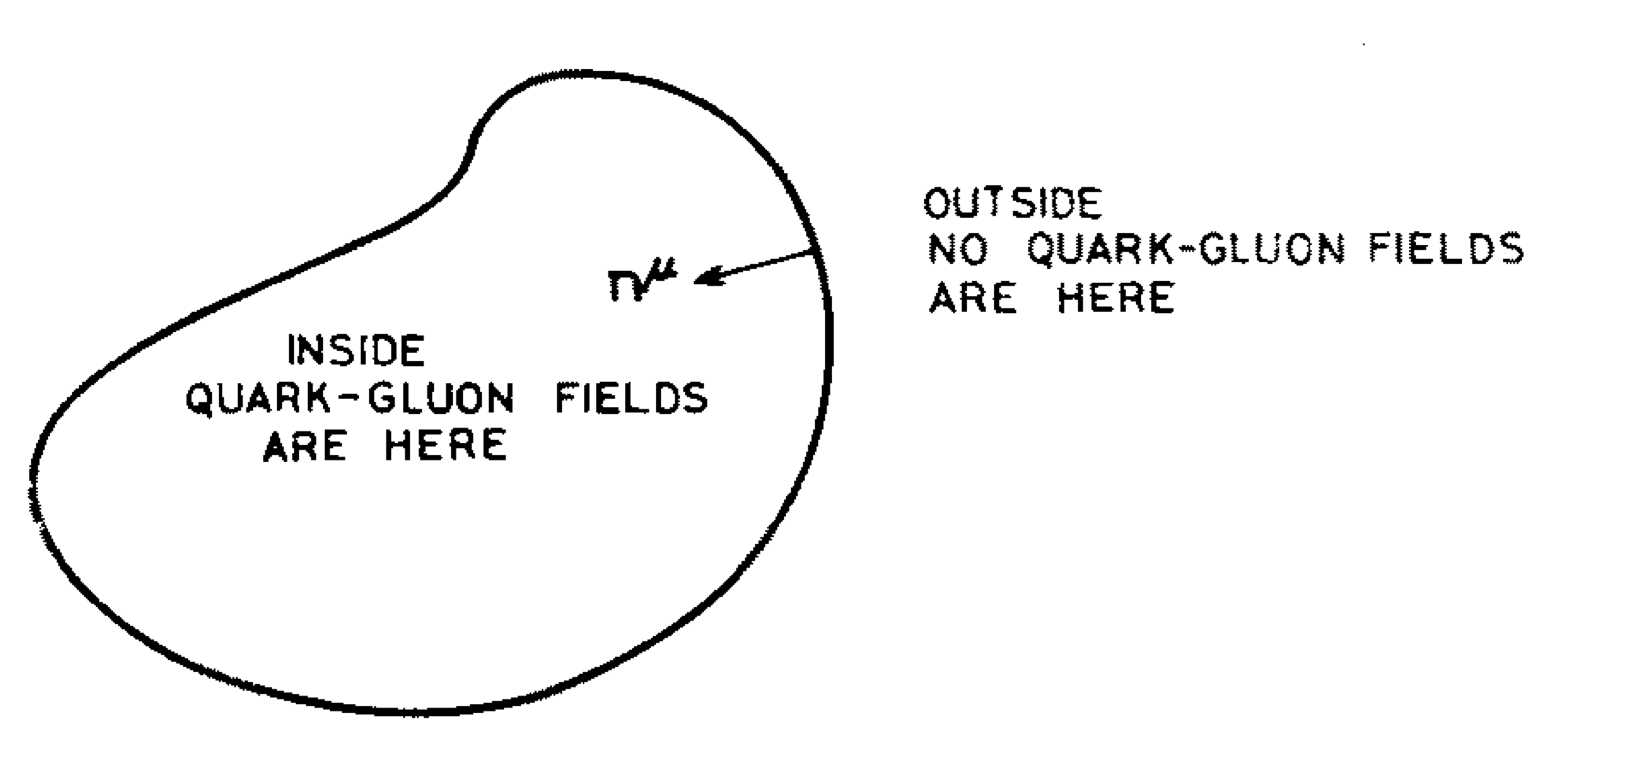
\includegraphics[width=0.4\textwidth]{./Images/Bag model BC.png}
    \caption[Diagrama de bolsa con condiciones de grontera]{\emph{Dentro de la bolsa se encuentran los quarks encerrados por la presión de la bolsa.}}
    \label{fig: Bolsa BC}
\end{wrapfigure}

\section{La aproximación de la cavidad esférica}

La aproximación de la cavidad esférica es una simplificación del modelo de bolsa que permite estudiar el comportamiento de los quarks dentro de un hadrón asumiendo que están confinados en una región esférica de radio ${R}_{0}$. En este enfoque, la dinámica de los quarks se describe mediante la ecuación de Dirac, y las condiciones de frontera en la superficie de la bolsa garantizan que los quarks no puedan escapar de la región confinada.

\hfill \break

La acción que describe este sistema está dada por:

\begin{equation}\label{eq-action}
W = \int \, \mathrm{d}t \left[ \int_{V} \mathrm{d}^{3} x \, \left( \frac{i}{2} \bar{\psi} \overleftrightarrow{\partial}_{\mu} {\gamma}^{\mu} \psi - \bar{\psi} m \psi - B \right) - \frac{1}{2} \int_{S} \mathrm{d}^{2} x \bar{\psi} \psi\right]
\end{equation}

donde $V$ es el volumen ocupado en la bolsa, $S$ es la superficie que encierra al volumen, $\psi$ es el espinor de campo de quark (${\gamma}^{\mu}$ son las \gls{gamma_matrices}), $\overleftrightarrow{\partial}_{\mu}$ es la derivada sobre lo de la derecha menos la derivada sobre lo de la izquierda, $m$ es la masa de los quarks que se mueven en la cavidad esférica que es la bolsa y $B$ es la presión de bolsa. 

La acción \eqref{eq-action} describe la dinámica de los quarks dentro de la bolsa. El primer término, $\frac{i}{2} \bar{\psi} \overleftrightarrow{\partial}_{\mu} {\gamma}^{\mu} \psi$, representa la energía cinética de los quarks, mientras que el segundo término, $\bar{\psi} m \psi$, corresponde a su energía de masa. El término $B$ introduce la presión de bolsa, que actúa como una energía de confinamiento que mantiene a los quarks dentro de la región esférica. Finalmente, el término superficial $\frac{1}{2} \int_{S} \mathrm{d}^{2} x \bar{\psi} \psi$ garantiza que los quarks no puedan escapar de la bolsa, imponiendo una condición de frontera efectiva para simular que los quarks se comporten como si tuvieran una masa infinita fuera de la bolsa, lo que impide su escape. % \acrshort{mit}. %\cite{MITBagModel}.

Las ecuaciones de movimiento y las condiciones de frontera se obtienen al extremizar la acción, ecuación \eqref{eq-action}, bajo variaciones en $\psi$ y $V$. La ecuación de Dirac dentro de la bolsa es:

\begin{equation}\label{eq-deq}
( i \slashed{\partial}_{\mu} - m) \psi= 0 \quad \mathrm{en} \, V,
\end{equation}

donde $\slashed{\partial}_{\mu} = {\partial}_{\mu} {\gamma}^{\mu}$. Las condiciones de frontera en la superficie $S$ son

% \begin{eqnarray}\label{eq-bc-deq}
% \left.
%     \begin{array}{c}
%         i {n}^{\mu} {\gamma}_{\mu} \psi = \psi \\ 
%         \frac{1}{2} {n}_{\mu} {\partial}^{\mu}(\bar{\psi} \psi) = B
%     \end{array} 
% \right\rbrace  \quad \mathrm{sobre} \, S,
% \end{eqnarray}

\begin{subequations}\label{eq-bc-deq}
    \begin{empheq}[right=\empheqrbrace \quad \text{sobre} \, S \text{,}]{align}
        i {n}^{\mu} {\gamma}_{\mu} \psi &= \psi \label{eq-bc-deq-a} \\
        \frac{1}{2} {n}_{\mu} {\partial}^{\mu}(\bar{\psi} \psi) &= B \label{eq-bc-deq-b}
    \end{empheq}
\end{subequations}

donde ${n}_{\mu}$ es la normal interior covariante a la superficie. La primera condición de frontera, ecuación \eqref{eq-bc-deq-a}, requiere que la componente normal del vector corriente ${J}_{\mu}=\bar{\psi}{\gamma}^{\mu}{\psi}$ se anule en la superficie, lo que conserva la corriente. La segunda condición, ecuación \eqref{eq-bc-deq-b}, requiere que la presión externa del campo de quarks se equilibre con la presión de bolsa $B$ (ver Fig. \ref{fig: Bolsa BC}). %[referencia MIT BM]. 50 Years of Quantum Chromodynamics

La solución general a las ecuaciones \eqref{eq-deq} y \eqref{eq-bc-deq-a} es una superposición de modos normales, cada uno caracterizado por un conjunto de números cuánticos $n$, $\kappa$, $j$, y $m$. 

\begin{equation}\label{eq-general-sol}
{\psi}_{\alpha}(x,t) = \sum_{n \kappa j m} N ({\omega}_{n \kappa j}) {a}_{\alpha} (n \kappa j m) {\psi}_{n \kappa k m} (x, t).
\end{equation}

donde:

\begin{itemize}
    \item[$\bullet$] $n$ es el número cuántico principal,
    \item[$\bullet$] $\kappa = \pm (j + \frac{1}{2})$ es el número cuántico de Dirac,
    \item[$\bullet$] $j$ y $m$ etiquetan el modo del momento angular y su componente $z$, respectivamente,
    \item[$\bullet$] $N({\omega}_{n \kappa j})$ es una constante de normalización,
    \item[$\bullet$] ${a}_{\alpha} (n \kappa j m)$ son los coeficientes de expansión que determinan la contribución de cada modo,
    \item[$\bullet$] y ${\psi}_{n \kappa k m} (x, t)$ son los modos normales de la ecuación de Dirac:
    \begin{equation}\label{eq-normal-modes}
        \psi_{n \kappa j m}(x, t) = \begin{pmatrix}
        f_{n \kappa j}(r) \, \Omega_{\kappa j m}(\theta, \phi) \\
        i g_{n \kappa j}(r) \, \Omega_{-\kappa j m}(\theta, \phi)
        \end{pmatrix} e^{-i \omega_{n \kappa j} t},
    \end{equation}
\end{itemize}

donde $f_{n \kappa j}(r)$ y $g_{n \kappa j}(r)$ son las funciones radiales, y $\Omega_{\kappa j m}(\theta, \phi)$ son las funciones angulares \cite{Chodos_1974}. %\cite{Chodos1974, "Relativistic Quantum Mechanics" por Bjorken y Drell, "Quantum Field Theory" por Itzykson y Zuber,"Introduction to Quantum Field Theory" por Peskin y Schroeder.}
Las frecuencias ${\omega}_{n \kappa j}$ se definen a partir de la expresión

\begin{equation}\label{eq-omega}
{\omega}_{n \kappa j} = \sqrt{{m}^{2} + {R}_{0}^{-2} {x}_{n \kappa j}^{2}},
\end{equation}

donde ${x}_{n \kappa j}$ son las soluciones de la ecuación trascendental a la que llegamos a partir de  \eqref{eq-bc-deq}.
La  condición de frontera cuadrática, la que está igualada a la presión de bolsa $B$ en \eqref{eq-bc-deq-b}, restringe los modos que pueden ser excitados. Entre otras cosas, permite sólo soluciones para la ecuación de Dirac. Para el caso de los quarks, $j = \frac{1}{2}$, ya sea $\kappa = - 1$,

\begin{equation}\label{eq-deq-sol-k=-1}
{\psi}_{n \, -1 \, \frac{1}{2} \, m} (x,t) = \frac{1}{\sqrt{4 \pi}} 
\left( 
\begin{array}{c}
i {j}_{0} ({\omega}_{n, \, -1} r / {R}_{0}) {U}_{m} \\
- {j}_{1} ({\omega}_{n, \, -1} r / {R}_{0}) \sigma \cdot \hat{r}{U}_{m} 
\end{array}
\right) \times {e}^{- i {\omega}_{n, \, -1} t / {R}_{0}}
\end{equation}

o ${\kappa} = 1$

\begin{equation}\label{eq-deq-sol-k=1}
{\psi}_{n \, 1 \, \frac{1}{2} \, m} (x,t) = \frac{1}{\sqrt{4 \pi}} 
\left( 
\begin{array}{c}
i{j}_{1} ({\omega}_{n, \, 1} r / {R}_{0}) \sigma \cdot \hat{r} {U}_{m} \\
{j}_{0} ({\omega}_{n, \, 1} r / {R}_{0}) {U}_{m} 
\end{array}
\right) \times {e}^{- i {\omega}_{n, \, 1} t / {R}_{0}}
\end{equation}

${U}_{m}$ es un espinor de Pauli bidimensional y ${j}_{\ell}(z)$ son las funciones de Bessel esféricas. Hemos omitido los índices $j$ sobre ${\omega}_{n \kappa}$ ya que solo $j = \frac{1}{2}$ es de interés en el presente (pues tratamos con partículas de \textit{espín} $\frac{1}{2}$, la cual es la componente angular total de los quarks). $N({\omega}_{n \kappa})$ es una constante de normalización escogida como

\begin{equation}
N({\omega}_{n \kappa}) \equiv \left( \frac{{\omega}_{n \kappa}^{\phantom{n \kappa} 3}}{2 {R}_{0}^{\phantom{0} 3} ({\omega}_{n \kappa} + \kappa) \sin^{2} {\omega}_{n \kappa}} \right)^{1/2}
\end{equation}

a partir de la restricción de normalización de \eqref{eq-general-sol} y la imposición de ortogonalidad sobre los modos normales, ecuación \eqref{eq-normal-modes}, es decir

\begin{equation}
    \int_{V} \mathrm{d}^{3} x \, \bar{\psi}_{n \kappa j m} (x) \psi_{n' \kappa' j' m'} (x) = \delta_{n n'} \delta_{\kappa \kappa'} \delta_{j j'} \delta_{m m'}.
\end{equation}

La condición de frontera lineal, ecuación \eqref{eq-bc-deq-a}, genera una condición eigenvalor para los modos de frecuencias ${\omega}_{n \kappa}$

\[
j_{0}(\omega_{n \kappa}) = - \kappa \, j_{1} (\omega_{n \kappa}),\footnote{
    Las funciones \( j_0(x) \) y \( j_1(x) \) son los armónicos esféricos de orden 0 y 1, respectivamente. Sus expresiones son:
    \[
    j_0(x) = \frac{\sin x}{x}, \quad j_1(x) = \frac{\sin x}{x^2} - \frac{\cos x}{x}.
    \]
}
\]

o 

\begin{equation}\label{eq-condeigenval}
\tan {\omega}_{n \kappa} = \frac{{\omega}_{n \kappa}}{{\omega}_{n \kappa} + \kappa}
\end{equation}

Por convención escogemos $n$ positiva (o negativa en dado caso que se escogieran modos de antipartículas, por ejemplo) secuencialmente para etiquetar las raíces positivas (o negativas) de la ecuación \eqref{eq-condeigenval} Las primeras soluciones a \eqref{eq-condeigenval} son 

\begin{equation}\label{eq-deq-sols}
\begin{array}{ccc}
\kappa = - 1: & {\omega}_{1 \, -1} = 2.04; & {\omega}_{2 \, -1} = 5.40 \\
\kappa = + 1: & {\omega}_{1 \, 1} = 3.81; & {\omega}_{2 \, 1} = 7.00.
\end{array}
\end{equation}

La condición de frontera cuadrática \eqref{eq-bc-deq-a} requiere que $\sum_{\alpha} (\partial / \partial r) \bar{\psi}_{\alpha} (x) {\psi}_{\alpha}(x)$ sea independiente de tiempo y dirección para $r={R}_{0}$ (lo que significa sobre la superficie de la bolsa). La independencia angular requiere que $j = \frac{1}{2}$. Para obtener independencia temporal, ajustamos

\begin{equation}\label{eq-condortogon}
\sum_{\alpha} {a}_{\alpha}^{*} (n \, \kappa \, j= \frac{1}{2} \, m) {a}_{\alpha} (n' \, \kappa' \, j= \frac{1}{2} \, m') = 0,
\end{equation}

a menos que $n = n'$, $\kappa = \kappa'$ o $n = -n'$, $\kappa = -\kappa'$ en cuyos casos no hay restricción ya que los términos dependientes del tiempo se cancela. La ecuación anterior es una restricción severa sobre los modos que deben ser ocupados. Deberíamos implementar la ecuación anterior requiriendo que para cada grado de libertad interno $\alpha$ sólo un modo normal, ${a}_{\alpha}(n \, \kappa \, j = \frac{1}{2} \, m)$ es excitado. Esto automáticamente será el caso para bariones de tres quarks si son requeridos a ser singletes de color.

Una vez que \eqref{eq-condortogon} es satisfecho, los términos independientes del tiempo en \eqref{eq-deq-sol-k=1} pueden ser coleccionados,

\begin{equation}
\sum_{\alpha \, n \, \kappa \, m} {\omega}_{n \kappa} {a}_{\alpha}^{*}(n \, \kappa \, \frac{1}{2} \, m) {a}_{\alpha}(n \, \kappa \, \frac{1}{2} \, m) = 4 \pi B {R}_{0}^{4},
\end{equation}

\begin{equation}
xd
\end{equation}


\subsubsection*{Conclusiones}

\begin{enumerate}

\item El campo en la bolsa se comporta sobre el promedio como un gas relativista perfecto; que es, la traza del tensor energía momento asociado con el campo, cuando es promediado sobre tiempo y espacio, es cero:
\begin{equation}
\left\langle \int_{R} {\mathrm{d}}^{3} x ({\Theta}_{\mu}^{\mu})_{\mathrm{campo}} \right\rangle = 0
\end{equation}
\item El volumen promediado en el tiempo de una bolsa es proporcional a su energía:
\begin{equation}
E = 4B \langle V \rangle
\end{equation}
\item El estado base y estados excitados más bajos de la bolsa contienen pocos partones de momento promedio de orden ${B}^{1/4}$ encerrados en un volumen de orden ${B}^{-3/4}$. [$B$ tiene la dimensión $(\mathrm{longitud})^{-4}$ con $\hbar=c=1$]
\item En el límite termodinámico la bolsa tiene una temperatura fija, ${T}_{0}$, independiente de su energía. ${T}_{0}$ es de orden ${B}^{-1/4}$. Esto es equivalente a las siguientes declaraciones
\begin{itemize}
\item La energía cinética promedio de los partones es de orden ${T}_{0}$ independiente de la energía de bolsa $E$ proporcionado el último es más grande que ${T}_{0}$: ${E} \gg {T}_{0}$.
\item La densidad de nivel asintótico ${\zeta(E)}$ del sistema es una función exponencial de $E$:
\[
\zeta \sim {e}^{E/{T}_{0}}
\]
\item El número, $N$, de partones más antipartones presente en el hadrón es proporcional a su energía:
\[
N \propto E/{T}_{0}
\]
\end{itemize}
\item Si la dinámica clásica es tal que hay un máximo momento angular del hadrón en una energía total dada $E$, ese máximo debe ser 
\[
{J}_{\mathrm{m\acute{a}x}} = \kappa {B}^{-1/3} {E}^{4 / 3},
\]
donde ${\kappa}$ es una constante adimensional determinada por la dinámica detallada. Si el límite clásico $({\hbar} \rightarrow 0)$ existe, las correcciones cuánticas a esta fórmula se reducirían por potencias de $E$. Si no hay trayectoria clásica a seguir, un argumento plausible sugiere que la trayectoría guía podría ser (para un gran $E$)
\[
{J}_{\mathrm{m\acute{a}x}} = {\kappa}' {B}^{-1/2} {E}^{2} \quad ({\hbar = 1}).
\]
\item El momento angular más probable para una $E$ grande está dada por 
\[
\bar{J} \propto ({B}^{-1/4} E)^{5/6}
\]
\end{enumerate}

%\subsection{Refinamientos que corrigen el movimiento del centro de masa}
%
%Una de las características incómodas de la aproximación de cavidad que es compartida por modelos de caparazón en general es que el centro de masa (c.m.) del estado de muchos cuerpos es en movimiento, y la energía cinética de movimiento es inevitablemente incluida en la energía orbital total. Esta contribución debería ser removida de la energía de bolsa para obtener la masa. En el modelo de caparazón nuclear es posible proyectar estados no relativistico de  momento definito de centro de masa. El Hamiltoniano cuántico invariante traslacionalmente subyacente es conocido, y la energía corregida del estado puede ser determinada (53). En la aproximación de cavidad, sin embargo, el Hamiltoniano cuántico es definido sólo con respecto a una cavidad particular y no es traslacionalmente invariante. No existe proyección sobre eigenestados de momento. 
%
%No hay procedimientos unívoco para corregir el movimiento de centro de masa. Sin embargo, varias aproximaciones han sido intentadas. En el método de Donoghue \& Johnson, el estado de bolsa con números cuánticos de nucleones no es precisamente identificado con el núcleon; en vez de eso, es considerado más generalmente como un paquete de ondas de estados de momentos de nucleones con un momento generalizado promedio $\langle \vb{p} \rangle = 0$ pero $\langle {p}^{2} \rangle \neq 0$. La energía de bolsa no es entonces precisamente la masa de la partícula, sino
%
%\begin{equation}
%{E}_{\mathrm{bolsa}} = \langle H \rangle =  \langle \sqrt{{p}^{2} + {m}^{2}} \rangle.
%\end{equation}
%
%Para la mayoría de estados (esos con $m \gg 1 / R$), la expansión no relativistica es posible: ${E}_{\mathrm{bolsa}}$. La corrección podría ser estimada en varias formas. 
%
%\section{Other models}
%
%\begin{equation}
%6
%\end{equation}

%
%\section{Una variedad de estados de bolsa}
%
%\subsection{Cuerdas}
%
%Las partículas de estado base han sido asumidas que corresponden a una bolsa esférica.
%

%\section{Interacciones}
%
%\subsection{Interacciones electrodébiles}
%
%El modelo de bolsa ha sido extensivamente usada como una herramienta en el estudio de las propiedades débiles y electromagnéticas de hadrones. No somos capaces de describir todas las aplicaciones, pero en vez de eso concentrar sobre las propiedades estáticas de los bariones (25, 34, 43, 86). Primero describimos los resultados no corregidos de (43). Cuatro tipos de corrección han sido estudiadas: 
%
%\begin{enumerate}
%\item retroceso del centro de masa
%\item intercambio de gluones
%\end{enumerate}
%
%Para el radio de carga del protón  DeGrand et al(43) obtiene
%
%$$
%\langle {r}^{2} \rangle_{\mathrm{EM}} = 0.55 {R}^{2} = (0.73 \; \mathrm{\unit{\femto\meter}})^{2}
%$$
%
%$$
%[\mathrm{experimento:} \quad \langle {r}^{2} \rangle_{\mathrm{EM}} = (0.90 \; \mathrm{\unit{\femto\meter}})^{2}]
%$$
%
%para quarks sin masa. [Para los valores de esta y otras cantidades en masa de quark no cero, ver (34, 86).] Este resultado es significante debido a que significa que el modelo de bolsa predice muy correctamente cercano el tamaño del protón. Tal conexión entre la masa y radio es no trivial. De hecho, usando el radio apropiado es a menudo más importante que tener la masa correcta, porque es el radio el que determina la escala de la mayoría de los elementos de matriz.
%
%El momento magnético de un estado puede ser calculado por el elemento de matriz del primer momento de corriente electromagnética
%
%\begin{equation}
%\langle \vb{\mu} \rangle = \langle \int \mathrm{d}^{3} x \frac{1}{2} \vb{x} \times \vb{J} (x) \rangle.
%\end{equation}
%
%Esta definición del momento incluye las contribuciones debida a ambas el flujo de carga y el espín del quark. En el límite no relativistíco, se reduce al usual
%
%\begin{equation}
%\vb{\mu} = \sum_{i} \frac{{Q}_{i} {\vb{\sigma}}_{i}}{2 {m}_{i}},
%\end{equation}
%
%mientras que para quarks sin masa en el protón, es
%
%\begin{equation}
%\vert {\mu}_{\mathrm{p}} \vert = 0.20 R e.
%\end{equation}
%
%Los parámetros de DeGrand et al llevan a una muy pequeña razón giromagnética (${g}_{\mathrm{p}} = 2{m}_{\mathrm{p}} {\mu}_{\mathrm{p}} / e = 1.9$)
\chapter{Estadística de Tsallis}\label{ch-Tsallis}

% \pagestyle{fancy}
% \fancyhead{} % clear all header fields
% \fancyhead[RO,LE]{\textbf{\chaptername\,\thechapter}  }
% \fancyfoot{} % clear all footer fields
% \fancyfoot[LE,RO]{\thepage}
% % \fancyfoot[LO,CE]{Introducción}
% \fancyfoot[CO,CE]{Estadística de Tsallis}

\section{Introducción}

La mecánica estadística estándar está basada en la entropía de \acrfull{bg}, \Gls{maths}, \Gls{tsallis}

\begin{equation}
{S}_{\mathrm{BG}} = - k \sum_{i=1}^{W} {p}_{i} \ln {p}_{i}, \quad \sum_{i=1}^{W} {p}_{i} = 1
\end{equation}

donde $W$ es el número de configuraciones microscópicas del sistema y ${p}_{i}$ es la probabilidad de acceder a la $i$-ésima configuración. Sin embargo, sistemas de no lineales dinámicos de muchos cuerpos requieren \emph{ergodicidad} (que su valor esperado sea igual a su promedio a largo plazo). Para sistemas no ergódicos, que sucede con sistemas complejos, no existe razón para usar estadística \acrshort{bg}. Por esta razón se ha requerido de una extensión para sistemas de este tipo, llamados \emph{no extensivos} (pues no son proporcional al número total de elementos del sistema), una de ellas es la siguiente, que extiende la entropía de \acrshort{bg} como

\begin{equation}
{S}_{q} = k \frac{1-\sum_{i} {p}_{i}^{q}}{q-1} \qquad (q\in \mathbb{R};\; {S}_{q=1} = {S}_{\mathrm{BG}})
\end{equation}

Bajo esta generalización, en un sistema constituido por dos subsistemas probabilisticamente independientes $A$ y $B$ (i.e., si ${p}_{ij}^{A+B} = {p}_{i}^{A}{p}_{j}^{B}$), entonces

\begin{equation}\label{eq-TsallisTwoSystems}
\frac{{S}_{{q}}(A+B)}{k} = \frac{{S}_{q}(A)}{k} + \frac{{S}_{q}(B)}{k} + (1 - q) \frac{{S}_{q}(A)}{k}\frac{{S}_{q}(B)}{k},
\end{equation}

(más adelante se usarán unidades naturales por lo que no aparecerá la constante de \acrshort{bg}, $k$) de donde se observa claramente que cuando $q=1$ se regresa a la estadística de \acrshort{bg} [ref Tsallis statistics].

NOTA: En la misma referencia se agrega la obtención de la energía de Tsallis para las masas

\section{Presión dentro del hadrón}\label{sec-PresTsa}

A partir de la ecuación \eqref{eq-TsallisTwoSystems}, podemos obtener la entropía dentro de un hadrón que consiste en una mezcla de gases quarks y gluon. De esta manera empezamos por considerar el cálculo de cada contribución, los quarks vistos como un gas ideal de Fermi ultrarelativista y los gluones vistos como un gas ideal de \acrfull{be}  ultrarelativista, ambos sin masa y no interactuantes, la interacción vendrá al final del parámetro $q$ de Tsallis

\subsection{Presión de gluones, un gas ideal de Bose - Einstein ultrarelativista}

Los níveles de energía de un bosón visto como un gas ideal de \acrshort{be} están dados por ${\epsilon}_{k}=cp=\hbar c k$, $p$ es la magnitud del momento de las partículas del gas, y $k$ la magnitud del vector de onda. Y la función de partición para un gas ideal de \acrshort{be} está determinada por:

\begin{equation}\label{eq-partfunc}
{\Xi}^{\mathrm{BE}}\left(T,V,\mu\right) = \prod_{k=1}^{\infty}\frac{1}{1-\xi {e}^{-\beta {\epsilon}_{k}}},
\end{equation}

donde $\beta = \frac{1}{kT}$, y ${\xi} = {e}^{\beta \mu}$ es la fugacidad del gas, $T$ es la temperatura del gas, $V$ el volumen del gas y $\mu$ el potencial químico del gas. El número de partículas promedio en cada estado de energía ${\epsilon}_{k}$ se calcula a través de la ecuación:

\begin{equation}\label{eq-avg-numb-parts}
\left\langle {n}_{k} \right\rangle = -\frac{1}{\beta} \frac{\partial}{\partial {\epsilon}_{k}} \ln {\Xi}^{\mathrm{BE}}\left.\right|_{\xi,V,{\epsilon}_{i \neq k}},
\end{equation}

\begin{equation}
\left\langle {n}_{k} \right\rangle = \frac{1}{{\xi}^{-1}{e}^{\beta{\epsilon}_{k}}-1} 
\end{equation}

De tal manera que el número total de partículas promedio y energía se pueden calcular como

\begin{equation}\label{eq-BE-Ntotal}
N(T,V,\mu)=\sum_{k}\left\langle {n}_{k} \right\rangle = \sum_{k}\frac{1}{{\xi}^{-1}{e}^{\beta{\epsilon}_{k}}-1}
\end{equation}

\begin{equation}\label{eq-BE-Etotal}
E(T,V,\mu) = \sum_{k}\left\langle {n}_{k} \right\rangle {\epsilon}_{k} = \sum_{k}\frac{{\epsilon}_{k}}{{\xi}^{-1}{e}^{\beta{\epsilon}_{k}}-1}.
\end{equation}

Para una gran cantidad de partículas, podemos sustituir la suma por una integral, considerando el número total de estados en el espacio fase clásico tenemos

\begin{equation}
\begin{split}
\Sigma &= \int \frac{\mathrm{d}^{3}r \mathrm{d}^{3}p}{{h}^{3}} \\ 
& = V\int \frac{4\pi {p}^{2} \mathrm{d}p}{{h}^{3}} \\
& = \frac{4\pi V}{{h}^{3}} \int_{0}^{\infty} {p}^{2} \mathrm{d} p 
\end{split}
\end{equation}

Usando la relación ${\epsilon}_{k} = cp$ obtenemos

\begin{equation}\label{eq-totalestados}
\Sigma = \frac{4\pi V}{(hc)^{3}} \int_{0}^{\infty} {\epsilon}^{2} \mathrm{d} \epsilon
\end{equation} 

De esta forma, sustituyendo \eqref{eq-totalestados} en \eqref{eq-BE-Ntotal} y \eqref{eq-BE-Etotal}, obtenemos

\begin{equation}\label{eq-BE-Ntotalint}
N(T,V,\mu) = \frac{4\pi V}{(hc)^{3}} \int_{0}^{\infty} \frac{{\epsilon}^{2} \mathrm{d} \epsilon}{{\xi}^{-1} {e}^{\beta \epsilon} - 1}
\end{equation}

\begin{equation}\label{eq-BE-Etotalint}
E(T,V,\mu) = \frac{4\pi V}{(hc)^{3}} \int_{0}^{\infty} \frac{{\epsilon}^{3} \mathrm{d} \epsilon}{{\xi}^{-1} {e}^{\beta \epsilon} - 1}
\end{equation}

Dado que tratamos con partículas sin masa, es posible tener infinitas partículas con energía ${\epsilon}_{0}=0$. De esta manera, el potencial químico $\mu$ debe ser cero pues es posible crear infinitas partículas con energía $0$ sin afectar a nuestros resultados puesto que no contribuyen a la energía total del sistema. Así, si $\mu=0$, entonces $\xi = 1$. Y sustituyendo en las ecuaciones \eqref{eq-BE-Ntotalint} y \eqref{eq-BE-Etotalint} obtenemos 

\begin{equation}\label{eq-BE-Ntotalintnofug}
N(T,V) = \frac{4\pi V}{(hc)^{3}} \int_{0}^{\infty} \frac{{\epsilon}^{2} \mathrm{d} \epsilon}{{e}^{\beta \epsilon} - 1}
\end{equation}

\begin{equation}\label{eq-BE-Etotalintnofug}
E(T,V) = \frac{4\pi V}{(hc)^{3}} \int_{0}^{\infty} \frac{{\epsilon}^{3} \mathrm{d} \epsilon}{ {e}^{\beta \epsilon} - 1}
\end{equation}

Para resolver las integrales, consideramos el cambio de variable $x=\beta \epsilon$, por lo que $\epsilon = \frac{x}{\beta}$ y así $\mathrm{d}\epsilon = \frac{\mathrm{d}x}{\beta}$ y así, entonces 

\begin{equation}\label{eq-BE-Ntotalintnofug-x}
N(T,V) = \frac{4\pi V}{(hc)^{3}} \frac{1}{{\beta}^{3}}\int_{0}^{\infty} \frac{{x}^{2} \mathrm{d} x}{{e}^{x} - 1}
\end{equation}

\begin{equation}\label{eq-BE-Etotalintnofug-x}
E(T,V) = \frac{4\pi V}{(hc)^{3}} \frac{1}{{\beta}^{4}} \int_{0}^{\infty} \frac{{x}^{3} \mathrm{d} x}{ {e}^{x} - 1}
\end{equation}

Con lo cual, obtenemos las funciones especiales ${g}_{n}(\xi)$ con $0 \leq \xi \leq 1$ tales que

\begin{equation}\label{eq-g-xi}
{g}_{n}(\xi) = \frac{1}{\Gamma(n)} \int_{0}^{\infty} \frac{{x}^{n-1} \mathrm{d}x}{{\xi}^{-1}{e}^{x}-1}
\end{equation}

Tal que las integrales de \eqref{eq-BE-Ntotalintnofug-x} y \eqref{eq-BE-Etotalintnofug-x} se vuelven

\begin{equation}\label{eq-sol-int-N}
\int_{0}^{\infty} \frac{{x}^{2} \mathrm{d} x}{ {e}^{x} - 1} = \Gamma(3) {g}_{3}(1)
\end{equation}

\begin{equation}\label{eq-sol-int-E}
\int_{0}^{\infty} \frac{{x}^{3} \mathrm{d} x}{ {e}^{x} - 1}= \Gamma(4) {g}_{4}(1)
\end{equation}

Sustituyendo las ecuaciones \eqref{eq-sol-int-N} y \eqref{eq-sol-int-E} en \eqref{eq-BE-Ntotalintnofug-x} y \eqref{eq-BE-Etotalintnofug-x}, respectivamente, y usando la propiedad ${g}_{n}(1) = \zeta(n)$, con $\zeta(n)$ representando la función zeta de Rienamann, se obtiene

\begin{equation}\label{eq-BE-Ntotalintreduced1}
N(T,V) = \frac{4\pi V}{(hc)^{3}} \frac{1}{{\beta}^{3}}\Gamma(3) \zeta(3)
\end{equation}

\begin{equation}\label{eq-BE-Etotalintreduced1}
E(T,V) = \frac{4\pi V}{(hc)^{3}} \frac{1}{{\beta}^{4}} \Gamma(4) \zeta(4)
\end{equation}

Ya que $\Gamma(n-1) = n!$ y $\zeta(4) = \frac{{\pi}^{4}}{90}$ se llega a

 \begin{equation}\label{eq-BE-Ntotalintreduced2}
N(T,V) = 8\pi V \left(\frac{kT}{hc} \right)^{3} \zeta(3)
\end{equation}

\begin{equation}\label{eq-BE-Etotalintreduced2}
E(T,V) = \frac{8\pi V}{(hc)^{3}} \left(k T \right)^{4} \frac{{\pi}^{4}}{30}
\end{equation}

Y usando unidades naturales $\hbar=k=x=1$ y $h=2\pi \hbar = 2\pi$, así entonces

 \begin{equation}\label{eq-BE-Ntotalintreduced3}
N(T,V) = \frac{1}{{\pi}^{2}} \zeta(3)V{T}^{3}
\end{equation}

\begin{equation}\label{eq-BE-Etotalintreduced3}
E(T,V) = \frac{{\pi}^{2}}{30} V{T}^{4}
\end{equation}

Finalmente, dado que hay tres componentes independientes de la carga de color, y consecuentemente $3 \times 3 - 1$ generadores de $SU(3)$, hay 8 diferentes tipos de gluones, y como cada gluón tiene dos proyecciones de espín, el factor de degeneración corresponde a ${g}_{G} = 8 \times 2 = 16$. Por lo tanto, pasamos a que las expresiones para el número total de gluones y la energía total de gluones como un gas ideal de \acrshort{be} ultrarrelativista son

 \begin{equation}\label{eq-BE-Ntotalgluons}
{N}_{G}(T,V) = \frac{{g}_{G}}{{\pi}^{2}} \zeta(3)V{T}^{3}
\end{equation}

\begin{equation}\label{eq-BE-Etotalgluons}
{E}_{G}(T,V) = {g}_{G}\frac{{\pi}^{2}}{30} V{T}^{4}
\end{equation}

Para calcular la contribución de presión debido a los gluones, partimos de la función de partición ${\Xi}^{BE}$ y el potencial macrocanónico o potencial gran canónico $\phi$

\begin{equation}\label{eq-BE-P1}
\begin{split}
\phi = -PV  & = -k T \ln {\Xi}^{BE} \\ 
\Rightarrow P & = \frac{kT}{V} \ln {\Xi}^{BE}
\end{split}
\end{equation}

Calculando el logaritmo de la función de partición \eqref{eq-partfunc} se tiene

\begin{equation}
\ln {\Xi}^{BE} = - \sum_{k=1}^{\infty} \ln\left(1 - \xi{e}^{-\beta {\epsilon}_{k}}\right)
\end{equation}

Nuevamente ocupamos el hecho de que son estados energéticos tan cercanos y tal cantidad de partículas en distintos estados energéticos, podemos sustituir la suma por una integral, usando el número total de estados \eqref{eq-totalestados} y el hecho de que no hay potencial químico ($\mu=0 \Rightarrow \xi=1$) para obtener

\begin{equation}
\ln {\Xi}^{BE} = - \frac{4\pi V}{(hc)^{3}} \int_{0}^{\infty} {\epsilon}^{2} \ln \left(1 - {e}^{-\beta\epsilon} \right) \mathrm{d} \epsilon
\end{equation}

Realizando la integral por partes tendremos

\begin{equation}
\begin{split}
\ln {\Xi}^{BE} & = - \frac{4\pi V}{(hc)^{3}} \left[ \left. \frac{1}{3} {\epsilon}^{3} \ln \left( 1 - {e}^{-\beta \epsilon}\right) \right|_{0}^{\infty} - \frac{1}{3} \beta \int_{0}^{\infty} \frac{{\epsilon}^{3} \mathrm{d}\epsilon}{{e}^{\beta \epsilon} - 1} \right] \\ 
& = \frac{4\pi V}{(hc)^{3}} \frac{kT}{3} \int_{0}^{\infty} \frac{{\epsilon}^{3} \mathrm{d} \epsilon}{{e}^{-\beta \epsilon} - 1}
\end{split}
\end{equation}

Resolviendo la integral, de la misma forma que con la ecuación \eqref{eq-BE-Etotalintnofug}, usando \eqref{eq-sol-int-E} y simplificando se llega a que la presión ejercida por un gas de partículas ultrarrelativistas tipo \acrshort{be}, usando la expresión \eqref{eq-BE-P1}, está dada como

\begin{equation}\label{eq-BE-P2}
P= \frac{1}{3} \frac{E}{V}
\end{equation}

Y dado que existen ${g}_{G}$ estados degenerados para la energía de los gluones, entonces, la presión correspondiente a los gluones es, usando \eqref{eq-BE-Etotalgluons},

\begin{equation}\label{eq-BE-Pgluons}
{P}_{G} = {g}_{G} \frac{{\pi}^{2}}{90}{T}^{4}
\end{equation}

Como cálculo final, hallamos la entropía a partir del potencial gran canónico por medio de la relación

\begin{equation}\label{eq-BE-Entropy}
\begin{split}
\phi &= E-TS-\mu N = -PV, \\
\Rightarrow S & = \frac{1}{T} \left(E+PV- \mu N \right)
\end{split}
\end{equation}

Sustituyendo la ecuación \eqref{eq-BE-P2} en \eqref{eq-BE-Entropy} y considerando $\mu=0$, la entropía del sistema es

\begin{equation}\label{eq-BE-S}
S = \frac{4}{3} \frac{E}{T}
\end{equation}

Y tomando en cuenta que tratamos con la energía de gluones \eqref{eq-BE-Etotalgluons}, la entropía del gas de gluones está dado como

\begin{equation}\label{eq-BE-Sgluons}
{S}_{G} = 4{g}_{G} \frac{{\pi}^{2}}{90}V{T}^{3}.
\end{equation}

\subsection{Presión de quarks, un gas ideal de Fermi - Dirac ultrarrelativista}\label{sec-Pquarks}

Las partículas ultrarelativistas tienen una relación energía-momento $\epsilon = \| \overrightarrow{p} \| c$\footnote{De la fórmula general $\epsilon = \sqrt{{p}^{2}{c}^{2} + {m}^{2}{c}^{4}}$, para masa en reposo despreciable.}.

Hay ciertos bosones con esta relación energía-momento, pero el número de fermiones con masa en reposo despreciable es muy poca. Para casos prácticos, ``despreciable'' significa una masa en reposo del orden de los neutrinos (${m}_{\nu} < 8 $eV). El gas ultrarelativistico de \acrfull{fd} puede ser visto como un gas caliente de fermiones con masa en reposo no despreciable, esto es, si el momento promedio en el gas es grande comparado con $mc$, es decir, si la energía térmica promedio $kT$ es grande comparada con la masa en reposo.

A partir de mecánica cuántica relativista, se sabe que uno puede crear pares de partículas y antipartículas (quarks y antiquarks, en nuestro caso) del vacío con un gasto energético de $2m{c}^{2}$. Por lo tanto, no debemos considerar un gas de partículas \acrshort{fd} solitarias, sino como pares partícula-antipartícula.

Así, trataremos con una mezcla de dos gases ideales \acrshort{fd}, entre las cuales, son posibles reacciones ``químicas''.

La función de partición para un gas ideal de \acrshort{fd}  está determinada por:

\begin{equation}
{\Xi}^{\mathrm{FD}}(T,V,\mu)=\prod_{k=1}^{\infty} \left(1 + \xi {e}^{-\beta {\epsilon}_{k}} \right)
\end{equation}

En este caso se considera una mezcla de gases (quarks y antiquarks), entonces la función de partición está dada como

\begin{equation}
\Xi\left(T,V,{\mu}_{+},{\mu}_{-}\right) = \prod_{{\epsilon}_{+}} \left(1+ {\xi}_{+}{e}^{-\beta {\epsilon}_{+}} \right) + \prod_{{\epsilon}_{-}} \left(1+ {\xi}_{-}{e}^{-\beta {\epsilon}_{-}} \right)
\end{equation}

donde ${\xi}_{+} = {e}^{\beta {\mu}_{+}}$ y ${\xi}_{-} = {e}^{\beta{\mu}_{-}}$ y el signo $+$ corresponde a las partículas mientras que el signo $-$ a las antipartículas. El número promedio de partículas en cada estado de energía se puede calcular usando la ecuación \eqref{eq-avg-numb-parts} y se obtiene

\begin{equation}\label{eq-FD-NumbParts}
\left\langle{n}_{k} \right\rangle = \frac{1}{{\xi}^{-1}{e}^{\beta{\epsilon}_{k}} + 1}
\end{equation}

por lo que el número total promedio para las partículas se calcularía a través de

\begin{equation}\label{eq-FD-Tot-Numb-Parts}
\begin{split}
{N}_{+}(T,V,{\mu}_{+}) &= \sum_{{\epsilon}_{+}} \left\langle{n}_{{\epsilon}_{+}} \right\rangle\\
& = \sum_{{\epsilon}_{+}} \frac{1}{{\xi}_{+}^{-1}{e}^{\beta{{\epsilon}}_{+}} + 1}
\end{split}
\end{equation}

Y de manera análoga se obtiene el número total promedio de antipartículas

\begin{equation}\label{eq-FD-Tot-Numb-Antiparts}
\begin{split}
{N}_{-}(T,V,{\mu}_{-}) &= \sum_{{\epsilon}_{-}} \left\langle{n}_{{\epsilon}_{-}} \right\rangle\\
& = \sum_{{\epsilon}_{-}} \frac{1}{{\xi}_{-}^{-1}{e}^{\beta{{\epsilon}}_{-}} + 1}
\end{split}
\end{equation}

En equilibrio termodinámico el número de promedio de partículas y antipartículas cambia constantemente debido al proceso de creación y aniquilación, por lo que no es conveniente fijar el número de ambas y posteriormente determinar los potenciales químicos. En lugar de ello, se realiza el siguiente análisis a fin de fijar el potencial químico.

Los cambios $d{N}_{+}$ y $d{N}_{-}$ de los dos números de partículas están relacionados por la relación

$$
d{N}_{+} = d{N}_{-}
$$

Las reacciones que suceden en el gas de quarks y antiquarks son de la forma

$$
q + \bar{q} \rightleftharpoons \, \mathrm{productos \; de \; reacci\acute{o}n} + \Delta E
$$

observamos que una antipartícula se crea o aniquila con cada partícula. Además, el resto de las partículas generadas por las reacciones creación-aniquilación no juegan un rol en el gas que estamos considerando de quarks antiquarks. Por esta razón, podemos notar que los potenciales químicos de partículas y antipartículas tienen que ser iguales con signos opuestos, ya que los productos de la reacción no contienen potencial químico,

\begin{equation}\label{eq-FD-chpot-fug}
{\mu}_{+} + {\mu}_{-} = 0, \quad {z}_{+}{z}_{-}=1
\end{equation}

Los números de partículas ${N}_{+}$ y ${N}_{-}$ no son independientes uno de otro, y por lo tanto no hay dos fugacidades independientes, sino en realidad solo uno. Sin embargo, en vez de ${N}_{+}$ y ${N}_{-}$ uno puede fijar la diferencia $N = {N}_{+} - {N}_{-}$, el excedente de partículas, yaa que no está influenciada por los procesos de creación y aniquilación:

\begin{equation}\label{eq-FD-ExcedenteNumParts}
\begin{split}
N & = {N}_{+} - {N}_{-} \\
& = \sum_{{\epsilon}_{+} > 0} \frac{1}{{\xi}_{+}^{-1}{e}^{\beta{{\epsilon}}_{+}} + 1} -\sum_{{\epsilon}_{-} > 0} \frac{1}{{\xi}_{-}^{-1}{e}^{\beta{{\epsilon}}_{-}} + 1}
\end{split}
\end{equation}

A partir de esta ecuación, uno determina la fugacidad tomando en cuenta la ecuación \eqref{eq-FD-chpot-fug}. En este sistema, el excedente $N$ de partículas no cambia por creación-aniquilación, pero el número de partículas medio ${N}_{+}$ y ${N}_{-}$ no puede ser controlado.

\begin{wrapfigure}{l}{0.35\textwidth}
\centering
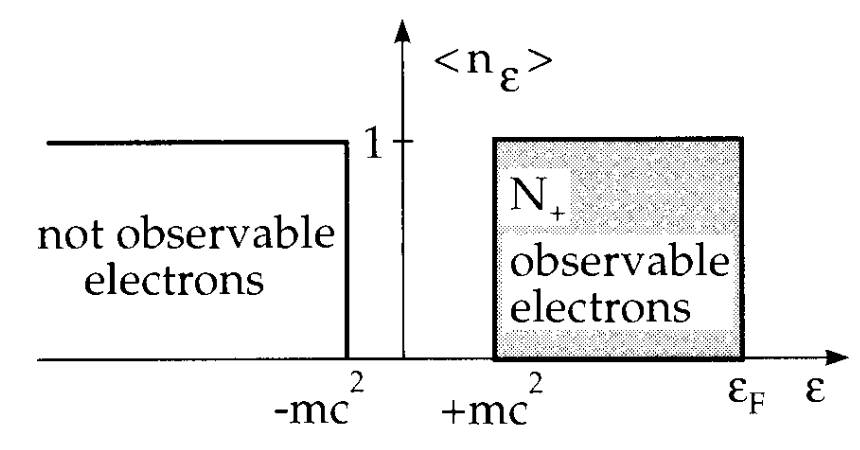
\includegraphics[width=0.35\textwidth]{./Images/ParticleNumberGaswithTnull.png}
\caption[Número de partículas para un gas de electrones a $T=0$]{\emph{$\left\langle {n}_{k} \right\rangle$ para un gas de electrones a $T=0$}}
\label{fig: Gas de electrones}
\end{wrapfigure}

Para explicar lo anterior, tenemos que considerar el espectro de energía de la ecuación libre de Dirac. En el caso ultrarelativista, $m \rightarrow 0$. En este espectro también hay estados de energía $\epsilon \leq -m {c}^{2}$ además de los estados de energía positiva $\epsilon \geq m{c}^{2}$. Uno puede describir ahora partículas y antipartículas en el espectro simultáneamente, si uno asume que en el vacío, sin partículas, todos los estados de energía negativa continua están ocupadas por electrones (inobservables).

En esta imagen de partículas (como son los electrones), en el continuo negativo (agujeros) son interpretados como antipartículas.

Para un gas de electrones con ${N}_{+}$ electrones y una energía de Fermi ${\epsilon}_{\mathrm{FD}} > m{c}^{2}$ tenemos en $T=0$ la situación de la figura \ref{fig: Gas de electrones}.

Si se aumenta la temperatura del gas de electrones, al principio, los electrones cerca de la energía de Fermi son excitados a estados más altos ${\epsilon} > {\epsilon}_{\mathrm{FD}}$. Esto ocurre en un rango de energía de anchura aproximada $kT$ alrededor de la energía de Fermi.

Sin embargo, si la temperatura es del orden de $2m{c}^{2}$, más y más electrones de un continuo más bajo pueden ser excitados en estados libres $\epsilon > {\epsilon}_{\mathrm{FD}}$. Estos electrones dejan huecos en el continuo más bajo, que representan positrones observables. El número de electrones observables también se incrementa. La diferencia ${N}_{+} - {N}_{-}$ sin embargo es la misma que antes. La energía negativa de los huecos ${\epsilon}_{\mathrm{huecos}} < - m{c}^{2}$ es simplemente relacionada a la energía positiva del positrón correspondiente como ${\epsilon}_{{e}^{+}} = - {\epsilon}_{\mathrm{hueco}}$.

El número de electrones y positrones observables puede ser calculado como sigue:

\begin{equation}\label{eq-FD-NumbPartsAndAntiparts}
{N}_{+} = \sum_{\epsilon>0} \left\langle {n}_{k} \right\rangle, \quad {N}_{-} = \sum_{\epsilon<0} \left(1 - \left\langle {n}_{k} \right\rangle \right)
\end{equation}

donde $\left\langle {n}_{k} \right\rangle$ está dado por \eqref{eq-FD-NumbParts} y ${\mu} = {\mu}_{+}$ como el potencial químico de los electrones (partículas). La expresión para ${N}_{-}$ puede ser transformada como

\begin{equation}\label{eq-FD-NumbTotAntiparts}
\begin{split}
{N}_{-} & = \sum_{\epsilon < 0} \left( 1 - \frac{1}{{\xi}^{-1}{e}^{\beta{\epsilon}} + 1} \right)  \\
& = \sum_{\epsilon < 0}\frac{{\xi}^{-1}{e}^{\beta \epsilon}}{{\xi}^{-1}{e}^{\beta{\epsilon}} + 1} \\
& = \sum_{\epsilon<0} \frac{1}{{\xi}{e}^{-\beta{\epsilon}} + 1}
\end{split}
\end{equation}

El espectro de energía de la ecuación libre de Dirac es simétrica alrededor de $\epsilon=0$. Así, uno puede sustituir $\epsilon \rightarrow -{\epsilon}_{-}$ en \eqref{eq-FD-NumbTotAntiparts} y entonces consideramos positrones con energía positiva.

\begin{equation}
{N}_{-} = \sum_{{\epsilon}_{-}>0} \frac{1}{{\xi}{e}^{\beta{\epsilon}_{-}}+1}
\end{equation}

Y por otro lado ${\xi} = {\xi}_{-}^{-1}$; es decir, ${\mu}_{+} = - {\mu}_{-}$. Ambas interpretaciones llevan a los mismos resultados, pero en algunos casos, la imagen de partícula-hueco de Dirac es más conveniente. Por ejemplo, el exceso de partículas en esta imagen es simplemente

\begin{equation}
\begin{split}
N & = {N}_{+} - {N}_{-} = \sum_{\epsilon > 0} \left\langle {n}_{\epsilon} \right\rangle - \sum_{\epsilon < 0} \left(1 - \left\langle {n}_{\epsilon} \right\rangle \right) \\
& = \sum_{\epsilon} \left\langle {n}_{\epsilon} \right\rangle  - \sum _{\epsilon < 0} 1 = \sum_{\epsilon} \left\langle {n}_{\epsilon} \right\rangle  - \sum_{\epsilon} \left\langle {n}_{\epsilon} \right\rangle ^{\mathrm{vac}}
\end{split}
\end{equation}


%%%%%%%%%%%%%%%%%%%%%%%%%%%%%%%%%%%%%%%%%%%
%%%%COMPLETAR EL RESTO DE LA EXPLICACIÓN%%%%%%%
%%%%%%%%%%%%%%%%%%%%%%%%%%%%%%%%%%%%%%%%%%%


Ahora procedemos con el cálculo de la presión. Tenemos que reescribir las sumas en la ecuación \eqref{eq-FD-ExcedenteNumParts}

\begin{equation}
{g}(\epsilon) = g \frac{4\pi V}{{h}^{3}{c}^{3}} {\epsilon}^{2}
\end{equation}

\begin{equation}
\ln \mathcal{Z} = g \frac{4 \pi V}{{h}^{3}{c}^{3}} \int_{0}^{\infty} {\epsilon}^{2} \, \mathrm{d} \epsilon \left[\ln \left( 1 + {e}^{-\beta \left(\epsilon - \mu \right)} \right) + \ln \left(1 + {e}^{-\beta \left(\epsilon + \mu\right)} \right) \right]
\end{equation}

de esta manera, podemos reescribir el número total de partículas 

\begin{equation}
N =\frac{4 \pi V}{(hc)^{3}} \left[ \int_{0}^{\infty} \frac{{\epsilon}^{2} \mathrm{d} \epsilon}{{e}^{\beta (\epsilon-\mu)} + 1} - \int_{0}^{\infty} \frac{{\epsilon}^{2} \mathrm{d} \epsilon}{{e}^{\beta (\epsilon+\mu)} + 1} \right] 
\end{equation}

Para la primera integral se hace el cambio de variable $x = \beta (\epsilon - \mu)$ por lo que  $\epsilon = \frac{x}{\beta} + \mu$ y $\mathrm{d} \epsilon = \frac{\mathrm{d}x }{\beta} $. Para la segunda, se hace $y = \beta(\epsilon + \mu)$ por lo que  $\epsilon = \frac{y}{\beta} - \mu$ y $\mathrm{d}\epsilon = \frac{\mathrm{d}y}{\beta}$. Y haciendo los respectivos cambios en los límites de integración, se obtiene 

\begin{equation}\label{eq-FD-int-Numb-Parts-Ints1}
N = \frac{4 \pi V}{(hc)^{3}} \frac{1}{\beta} \left[ \int_{-\beta \mu}^{\infty} \frac{(\frac{x}{\beta} + \mu)^{2}}{{e}^{x}+1}  \mathrm{d}x - \int_{\beta \mu}^{\infty} \frac{(\frac{y}{\beta} - \mu)^{2}}{{e}^{y}+1}  \mathrm{d}y \right]
\end{equation}

Factorizando el término $\beta$ en los numeradores de \eqref{eq-FD-int-Numb-Parts-Ints1} y reacomodando los límites de integración,podemos reescribir

\begin{equation}\label{eq-FD-int-Numb-Parts-Ints2}
\begin{split}
N &= \frac{4 \pi V}{(hc)^{3}} \frac{1}{{\beta}^{3}} \left[\int_{-\beta \mu}^{\infty} \frac{(x + \beta \mu)^{2}}{{e}^{x}+1}  \mathrm{d}x - \int_{\beta \mu}^{\infty} \frac{(y -\beta \mu)^{2}}{{e}^{y}+1}  \mathrm{d}y \right] \\
& = \frac{4 \pi V}{(hc)^{3}} \frac{1}{{\beta}^{3}} \left[ \int_{-\beta \mu}^{0} \frac{(x + \beta \mu)^{2}}{{e}^{x}+1}  \mathrm{d}x + \int_{0}^{\infty} \frac{(x + \beta \mu)^{2}}{{e}^{x}+1}\mathrm{d}x \right. \\
& \left. - \int_{\beta \mu}^{0} \frac{(y -\beta \mu)^{2}}{{e}^{y}+1}  \mathrm{d}y  - \int_{0}^{\infty} \frac{(y -\beta \mu)^{2}}{{e}^{y}+1}  \mathrm{d}y  \right]
\end{split}
\end{equation}

Juntando las integrales que van de cero a infinito en \eqref{eq-FD-int-Numb-Parts-Ints2}, y reemplazando $y \rightarrow x$, se tiene

\begin{equation}\label{eq-FD-int-Numb-Parts-IntsPart1-2}
\begin{split}
\int_{0}^{\infty} \frac{(x + \beta \mu)^{2}}{{e}^{x}+1}\mathrm{d}x - \int_{0}^{\infty} \frac{(y -\beta \mu)^{2}}{{e}^{y}+1}  \mathrm{d}y & = \int_{0}^{\infty} \frac{(x +\beta \mu)^{2} - (x -\beta \mu)^{2}}{{e}^{y}+1}  \mathrm{d}y \\
& = 4\beta \mu \int_{0}^{\infty} \frac{x}{{e}^{x} + 1} \mathrm{d} x.
\end{split}
\end{equation}

Podemos juntar el resto de las integrales si trabajamos una de ellas con un cambio de variable para ajustar los límites integrales a los mismos $y \rightarrow -x$, como

\begin{equation}
\begin{split}
- \int_{\beta \mu}^{0} \frac{(y -\beta \mu)^{2}}{{e}^{y}+1}  \mathrm{d}y & =  \int_{0}^{\beta \mu} \frac{(y -\beta \mu)^{2}}{{e}^{y}+1}  \mathrm{d}y \\
& = - \int_{0}^{-\beta \mu} \frac{(-x -\beta \mu)^{2}}{{e}^{-x}+1}  \mathrm{d}x \\
& = \int_{-\beta \mu}^{0} \frac{(x + \beta \mu)^{2}}{{e}^{-x}+1}  \mathrm{d}x
\end{split}
\end{equation}

Y de esta manera

\begin{equation}\label{eq-FD-int-Numb-Parts-IntsPart2-2}
\begin{split}
\int_{-\beta \mu}^{0} \frac{(x + \beta \mu)^{2}}{{e}^{x}+1}  \mathrm{d}x - \int_{\beta \mu}^{0} \frac{(y -\beta \mu)^{2}}{{e}^{y}+1}  \mathrm{d}y & = \int_{-\beta \mu}^{0} \frac{(x + \beta \mu)^{2}}{{e}^{x}+1}  \mathrm{d}x  +  \int_{-\beta \mu}^{0} \frac{(x + \beta \mu)^{2}}{{e}^{-x}+1}  \mathrm{d}x \\ 
& =  \int_{-\beta \mu}^{0} (x + \beta \mu)^{2} \left[\frac{1}{{e}^{x} + 1} + \frac{1}{{e}^{-x} + 1} \right] \mathrm{d}x \\
& = \int_{-\beta \mu}^{0} (x + \beta \mu)^{2} \mathrm{d}x
\end{split}
\end{equation}

Dado que en el paréntesis cuadrado de \eqref{eq-FD-int-Numb-Parts-IntsPart2-2}, al multiplicar por ${e}^{x}$ el segundo término, se llega a que los dos términos dentro del paréntesis dan la unidad. De esta manera, el número de partículas, sustituyendo \eqref{eq-FD-int-Numb-Parts-IntsPart1-2} y \eqref{eq-FD-int-Numb-Parts-IntsPart2-2} en \eqref{eq-FD-int-Numb-Parts-Ints2}

\begin{equation}
N = \frac{4 \pi V}{(hc)^{3}} \frac{1}{{\beta}^{3}} \left[4\beta \mu \int_{0}^{\infty} \frac{x}{{e}^{x} + 1} \mathrm{d} x + \int_{-\beta \mu}^{0} (x + \beta \mu)^{2} \mathrm{d}x \right]
\end{equation}

Haciendo el cambio de variable ${z} = x + \beta \mu$ en la última integral se obtiene

\begin{equation}\label{eq-FD-int-Numb-Parts-Ints3}
N = \frac{4 \pi V}{(hc)^{3}} \frac{1}{{\beta}^{3}} \left[4\beta \mu \int_{0}^{\infty} \frac{x}{{e}^{x} + 1} \mathrm{d} x + \int_{0}^{\beta \mu} {z}^{2} \mathrm{d}z \right]
\end{equation}

Y de manera análoga a lo que es la función \eqref{eq-g-xi}, tenemos las funciones especiales ${f}_{n}(\xi)$ con $0 \leq \xi \leq 1$:

\begin{equation}\label{eq-f-xi}
{f}_{n}(\xi) = \frac{1}{\Gamma(n)} \int_{0}^{\infty} \frac{{x}^{n-1} \mathrm{d}x}{{\xi}^{-1}{e}^{x} + 1}
\end{equation}

Entonces la primera integral de \eqref{eq-FD-int-Numb-Parts-Ints3} se vuelve

\begin{equation}
\int_{0}^{\infty} \frac{x}{{e}^{x} + 1} \mathrm{d} x = \Gamma(2) {f}_{2}(1) = {f}_{2}(1)
\end{equation}

Por último, las funciones ${f}_{n}(\xi)$ cumplen con la propiedad:

\begin{equation}\label{eq-f-xi=1}
{f}_{n}(1) = \left(1 - \frac{1}{{2}^{n-1}} \right) \zeta (n)
\end{equation}

Usando la ecuación \eqref{eq-f-xi=1} y que $\zeta(2)= \displaystyle \frac{{\pi}^{2}}{6}$ en la primera integral de \eqref{eq-FD-int-Numb-Parts-Ints3}, se obtiene

\begin{equation}\label{eq-FD-int-Numb-Parts-Ints3-1/2}
\int_{0}^{\infty} \frac{x}{{e}^{x} + 1} \mathrm{d} x = \frac{{\pi}^{2}}{12}
\end{equation}

Y para la segunda integral, se obtiene simplemente

\begin{equation}\label{eq-FD-int-Numb-Parts-Ints3-2/2}
\int_{0}^{\beta \mu} {z}^{2} \mathrm{d}z = \frac{(\beta \mu)^{3}}{3}
\end{equation}

Sustituyendo \eqref{eq-FD-int-Numb-Parts-Ints3-1/2} y \eqref{eq-FD-int-Numb-Parts-Ints3-2/2} en \eqref{eq-FD-int-Numb-Parts-Ints3} se llega a la expresión

\begin{equation}
\begin{split}
N & = \frac{4 \pi V}{(hc)^{3}} \frac{1}{{\beta}^{3}} \left[4 \beta \mu \frac{{\pi}^{2}}{12} + \frac{(\beta \mu)^{3}}{3} \right] \\
& = 4 \pi V \left(\frac{kT}{hc} \right)^{3} \left[ \frac{{\pi}^{2}}{3} \left(\frac{\mu}{kT}\right) + \frac{1}{3} \left(\frac{\mu}{kT} \right)^{3} \right]
\end{split}
\end{equation}

Y ahora, analógamente con el gas ideal de \acrshort{be}, la expresión se reescribe en unidades naturales usando $c=\hbar = k = 1$ y $h = 2\pi$, y se agrega el factor de degeneración de los quarks ${g}_{Q}$

\begin{equation}\label{eq-FD-Total-Number-Particles-Quarks}
{N}_{Q} = \frac{{g}_{Q}}{6} \left[\frac{\mu}{T} + \frac{1}{{\pi}^{2}} \left(\frac{\mu}{T} \right)^{3} \right] V{T}^{3}
\end{equation}

El factor de degeneración de los quarks se compone del producto del número de proyecciones de espín (${N}_{s}$), el número de colores, ${N}_{c}$, y el número de sabores, ${N}_{f}$, a consideración ${g}_{G}={N}_{s}{N}_{c}{N}_{f}$. Para este caso, se tienen ${N}_{s}=2$ proyecciones de espín, ${N}_{c}=3$ colores y ${N}_{f}=2$ sabores, $u$ y $d$, dado que bajo este esquema, analizamos materia nuclear ordinaria. Por tanto ${g}_{Q}=12$.

Para calcular la contribución de los quarks y antiquarks a la energía del sistema, se considera

\begin{equation}
E = {E}_{+} + {E}_{-} = \sum_{{\epsilon}_{+}>0} \left\langle{n}_{{\epsilon}_{+}} \right\rangle {\epsilon}_{+} + \sum_{{\epsilon}_{-}>0} \left\langle{n}_{{\epsilon}_{-}} \right\rangle {\epsilon}_{-} 
\end{equation}

donde ${E}_{+}$ es la energía de los quarks y ${E}_{-}$ de los antiquarks. Usando la ecuación \eqref{eq-FD-NumbParts}, y la relación entre las fugacidades explicada con anterioridad \eqref{eq-FD-chpot-fug}, podemos establecer que 

\begin{equation}\label{eq-FD-Quark-Energy-Ints}
\begin{split}
E & = \sum_{{\epsilon}_{+} > 0} \frac{{\epsilon}_{+}}{{e}^{\beta({\epsilon}_{+}-\mu)} + 1} + \sum_{{\epsilon}_{-} > 0} \frac{{\epsilon}_{-}}{{e}^{\beta({\epsilon}_{-}+\mu)} + 1} \\
& \Rightarrow \frac{4{\pi}V}{(hc)^{3}} \left[ \int_{0}^{\infty}  \frac{{\epsilon}^{3} \mathrm{d} \epsilon}{{e}^{\beta({\epsilon}-\mu)} + 1}+ \int_{0}^{\infty}\frac{{\epsilon}^{3} \mathrm{d} \epsilon}{{e}^{\beta({\epsilon}+\mu)} + 1} \right]
\end{split}
\end{equation}

Donde se ha usado el número total de estados en el espacio fase clásico \eqref{eq-totalestados}. A partir de aquí, se procede a hacer el mismo procedimiento que para el cálculo del número total de partículas para resolver las integrales \eqref{eq-FD-Quark-Energy-Ints}, de lo que se llega fácilmente a que 

\begin{equation}\label{eq-FD-Quark-Energy-Ints2}
\begin{split}
E & = \frac{4\pi V}{(hc)^{3}} \frac{1}{{\beta}^{4}} \left[2\int_{0}^{\infty} \frac{{x}^{3}}{{e}^{x} + 1} \mathrm{d}x + 6(\beta \mu)^{2} \int_{0}^{\infty} \frac{x}{{e}^{x}+1} \mathrm{d}x + \int_{-\beta \mu}^{0} \left(x + \beta \mu \right)^{3} \mathrm{d}x \right] \\
& = \frac{4\pi V}{(hc)^{3}} \frac{1}{{\beta}^{4}} \left[2\int_{0}^{\infty} \frac{{x}^{3}}{{e}^{x} + 1} \mathrm{d}x + 6(\beta \mu)^{2} \int_{0}^{\infty} \frac{x}{{e}^{x}+1} \mathrm{d}x + \int_{0}^{\beta \mu} {z}^{3} \mathrm{d}z \right]
\end{split}
\end{equation}

Donde se ha usado el cambio de variable $z=x+\beta \mu$ para la última integral. Para resolver las primeras integrales, hacemos uso de las funciones \eqref{eq-f-xi}

\begin{equation}\label{eq-FD-Quark-Energy-Ints-1/3}
\int_{0}^{\infty} \frac{{x}^{3}}{{e}^{x} + 1} \mathrm{d} x = \Gamma(4){f}_{4}(1) = \frac{7{\pi}^{4}}{120}
\end{equation}

La segunda integral se obtuvo con anterioridad \eqref{eq-FD-int-Numb-Parts-Ints3-1/2}, y la tercera se cálcula directamente como

\begin{equation}\label{eq-FD-Quark-Energy-Ints-3/3}
\int_{0}^{\beta \mu}{z}^{3} \mathrm{d}z = \frac{(\beta\mu)^{4}}{4}
\end{equation}

Así, sustituyendo las ecuaciones \eqref{eq-FD-Quark-Energy-Ints-1/3}, \eqref{eq-FD-int-Numb-Parts-Ints3-1/2} y \eqref{eq-FD-Quark-Energy-Ints-3/3} en \eqref{eq-FD-Quark-Energy-Ints2}, obtenemos

\begin{equation}
\begin{split}
E & = \frac{4\pi V}{(hc)^{3}} \frac{1}{{\beta}^{4}}  \left[2 \left(\frac{7{\pi}^{4}}{120} \right) + 6 (\beta \mu)^{2} \frac{{\pi}^{2}}{12} + \frac{1}{4}(\beta \mu)^{4}\right] \\
& = \frac{4\pi V}{(hc)^{3}} (kT)^{4} \left[\frac{7{\pi}^{4}}{60} + \frac{{\pi}^{2}}{2} \left(\frac{\mu}{kT} \right)^{2} + \frac{1}{4} \left(\frac{\mu}{kT} \right)^{4}\right]
\end{split}
\end{equation}

Finalmente, usando unidades naturales como con el número de partículas, y agregando el factor de degeneración, obtenemos la energía del gas de quarks - antiquarks

\begin{equation}\label{eq-FD-Quark-Energy}
{E}_{Q} = {g}_{Q} \left[\frac{7{\pi}^{2}}{120} + \frac{1}{4} \left(\frac{\mu}{T} \right)^{2} + \frac{1}{8{\pi}^{2}} \left(\frac{\mu}{T} \right)^{4}\right]V{T}^{4}
\end{equation}

Para finalizar el cálculo de cantidades termodinámicas en este modelo, calculamos la presión producida por los quarks y antiquarks de manera análoga como con los gluones. La presión está definida por la ecuación \eqref{eq-BE-P1}, entonces para este caso, tenemos la función de partición que está dada como

\begin{equation}\label{eq-FD-Log-Part-Func}
\begin{split}
\ln \Xi &= \sum_{{\epsilon}_{+}} \ln \left(1+{e}^{-\beta({\epsilon}_{+}-\mu)} \right) + \sum_{{\epsilon}_{-}} \ln \left(1+{e}^{-\beta({\epsilon}_{-}+\mu)} \right) \\ 
& \Rightarrow \frac{4 \pi V}{(hc)^{3}} \left[ \int_{0}^{\infty} {\epsilon}^{2} \ln \left(1 + {e}^{-\beta(\epsilon - \mu)} \right) \mathrm{d}\epsilon + \int_{0}^{\infty} {\epsilon}^{2} \ln \left(1 + {e}^{-\beta(\epsilon + \mu)} \right) \right]
\end{split}
\end{equation}

donde se han reemplazado las sumas por las integrales. Para resolver las integrales, ocupamos integración por partes, para la primera integral tenemos

\begin{equation}\label{eq-FD-Log-Part-Func-Int1}
\begin{split}
\int_{0}^{\infty} {\epsilon}^{2} \ln \left(1 + {e}^{-\beta(\epsilon-\mu)} \right) \mathrm{d} \epsilon & = \left. \frac{{\epsilon}^{3}}{3} \ln \left(1+{e}^{-\beta(\epsilon-\mu)} \right) \right|_{0}^{\infty} + \frac{\beta}{3} \int_{0}^{\infty} \frac{ {\epsilon}^{3} \mathrm{d} \epsilon}{{e}^{\beta(\epsilon - \mu)} + 1} \\
& = \frac{\beta}{3} \int_{0}^{\infty} \frac{{\epsilon}^{3} \mathrm{d} \epsilon}{{e}^{\beta (\epsilon - \mu)} + 1 }
\end{split}
\end{equation}

En el cual, después de evaluar en los límites en la ecuación \eqref{eq-FD-Log-Part-Func-Int1}, se llega a que se cancela el primer término. Para la segunda integral de \eqref{eq-FD-Log-Part-Func} se procede similarmente y se obtiene

\begin{equation}\label{eq-FD-Log-Part-Func-Int2}
\int_{0}^{\infty} {\epsilon}^{2} \ln \left(1 + {e}^{-\beta(\epsilon + \mu)} \right) = \frac{\beta}{3} \int_{0}^{\infty} \frac{{\epsilon}^{3} \mathrm{d} \epsilon}{{e}^{\beta (\epsilon + \mu)} + 1 }
\end{equation}

Y, sustituyendo las ecuaciones \eqref{eq-FD-Log-Part-Func-Int1} y  \eqref{eq-FD-Log-Part-Func-Int2} en \eqref{eq-FD-Log-Part-Func}, obtenemos 

\begin{equation}
\ln \Xi = \frac{4\pi V }{(hc)^{3}} \frac{\beta}{3} \left[\int_{0}^{\infty} \frac{{\epsilon}^{3} \mathrm{d} \epsilon}{{e}^{\beta (\epsilon - \mu)} + 1 } + \int_{0}^{\infty} \frac{{\epsilon}^{3} \mathrm{d} \epsilon}{{e}^{\beta (\epsilon + \mu)} + 1 }\right]
\end{equation}

Y, volviendo con la expresión \eqref{eq-BE-P1}, podemos reescribirla aprovechando la expresión integral \eqref{eq-FD-Quark-Energy-Ints}, para obtener la expresión de presión total de gluones con unidades naturales como

\begin{equation}
P = \frac{1}{3} \frac{E}{V}
\end{equation}

Y sustituyendo para el caso de la energía de quarks ${E}_{Q}$ \eqref{eq-FD-Quark-Energy} en la exprsión anterior, obtenemos

\begin{equation}\label{eq-FD-Quark-Pressure}
{P}_{Q} = \frac{{g}_{Q}}{3} \left[\frac{7 {\pi}^{2}}{120} + \frac{1}{4} \left(\frac{\mu}{T} \right)^{2} \frac{1}{8{\pi}^{2}} \left(\frac{\mu}{T} \right)^{4} \right] {T}^{4}
\end{equation}

La entropía se puede calcular a partir de una expresión similar a \eqref{eq-BE-Entropy}, la cual es

\begin{equation}
\phi = E -TS - \sum_{i}{\mu}_{i} {N}_{i} = - PV
\end{equation}

\begin{equation}
S = \frac{1}{T} \left(E + PV - \sum_{i} {\mu}_{i} {N}_{i} \right)
\end{equation}

donde la suma es sobre todas las especies de partículas, en este caso quarks y antiquarks. Por tanto, para el caso del gas de Fermi, tenemos 

\begin{equation}\label{eq-FD-Entropy}
\begin{split}
S & = \frac{1}{T} \left(E + PV - {\mu}_{+} {N}_{+} - {\mu}_{-} {N}_{-} \right)\\
& = \frac{1}{T} \left(E + PV - \mu V \right) \\
& = \frac{4}{3} \frac{E}{T} - \mu \frac{N}{T}
\end{split}
\end{equation}

donde se ha usado el hecho de que ${\mu}_{+} = \mu$ y ${\mu}_{-} = - \mu$. Y sustituyendo las ecuaciones \eqref{eq-FD-Quark-Energy} y \eqref{eq-FD-Total-Number-Particles-Quarks} en \eqref{eq-FD-Entropy}, obtenemos la entropía de los quarks

\begin{equation}\label{eq-FD-Quark-Entropy}
{S}_{Q} = {g}_{Q} \left[\frac{7{\pi}^{2}}{90} + \frac{1}{6} \left(\frac{\mu}{T} \right)^{2} \right]V{T}^{3}
\end{equation}

donde se ha considerado el factor de degeneración ${g}_{Q} = 12$ correspondiente de este gas de quarks.

\section{El protón en el modelo de Tsallis}

\subsection{La entropía en el modelo de Tsallis}

Consideramos protones como un gas de quarks y gluones. En esta formulación de sistemas no extensivos con dos componentes. La correlación entre las dos especies son representadas por el valor del parámetro de Tsallis $q$. La entropía no extensiva para un sistema constituido de dos subsistemas $A$ y $B$ está dada por la ecuación \eqref{eq-TsallisTwoSystems}. En este caso, los subsistemas son los dos gases constituidos de quarks (Q) y gluones (G), donde el gas de quarks es una mezcla conjunta de quarks y antiquarks como se ha explicado en la sección \ref{sec-Pquarks}. Con todo esto en consideración, la entropía del protón está dada, considerando unidades naturales, como

\begin{equation}
{S}_{q}(Q+G) = {S}_{q}(Q) + {S}_{q}(G) + (1-q){S}_{q}(Q){S}_{q}(G)
\end{equation}

donde ${S}_{q}(Q)$ representa la entropía de Tsallis de los quarks, ${S}_{q}(G)$ es la entropía de Tsallis de los gluones y ${S}_{q}(Q+G)$ es la entropía del sistema conjunto, considerando que el último término, ese con el factor de Tsallis $q$, es el que contiene toda la información de la interacción de los subsistemas (las autointeracciones se excluyen en esta primera aproximación).

La interacción fuerte entre los subsistemas debe tener efectos sobre las propiedades físicas del sistema quark-gluon. Las correlaciones deben modificar el comportamiento de las propiedades termodinámicas. Ello conlleva a cambiar la forma de calcular estas propiedades. Es así  que, en analogía con la entropía de Tsallis para dos subsistemas probabilísticamente independientes, proponemos la entropía del sistema como

\begin{equation}\label{eq-Entropy-Quark-Gluon}
{S}_{q}(Q + G) = {S}_{1}(Q) + {S}_{1}(G) + (1-q){S}_{1}(Q){S}_{1}(G)
\end{equation}

donde, como podrá notarse, se ha hecho que ambos subsistemas se consideran como esos de \acrshort{bg} convencional, esto equivale a excluir la interacción dentro de cada subsistema, de tal manera que el parámetro $q$ de Tsallis es el que introduce toda la interacción entre los subsistemas en el término cruzado de \eqref{eq-Entropy-Quark-Gluon}. Así, cuando $q=1$ en \eqref{eq-Entropy-Quark-Gluon}, se recuperará la entropía total correspondiente a la suma de las ecuaciones \eqref{eq-BE-Sgluons} y \eqref{eq-FD-Quark-Entropy}

\begin{equation}\label{eq-total-entropy-quarks-gluons}
\begin{split}
{S}_{Q+G} & = {S}_{Q} +{S}_{G} \\
& = {g}_{Q} \left[ \frac{7{\pi}^{2}}{90} + \frac{1}{6} \left(\frac{\mu}{T} \right)^{2}\right] V{T}^{3} + 4{g}_{G} \frac{{\pi}^{2}}{90} V{T}^{3} \\
& = \left[\frac{74{\pi}^{2}}{45} + 2 \left(\frac{\mu}{T} \right)^{2} \right]V{T}^{3}
\end{split}
\end{equation}

Donde la última igualdad de \eqref{eq-total-entropy-quarks-gluons}, se obtiene al sustituir los valores de los factores de degeneración correspondientes de quarks y gluones. Cabe notar que ${S}_{Q+G}$ corresponderá igualmente a la entropía en un marco de \acrshort{bg}. 

De esta manera, podemos reescribir la ecuación \eqref{eq-Entropy-Quark-Gluon} como

\begin{equation} 
{S}_{q} = {S}_{Q} + {S}_{G} + (1-q) {S}_{Q}{S}_{G}
\end{equation}

donde las entropías de los subsistemas de quarks y de gluones ya se han definido por las ecuaciones  \eqref{eq-BE-Sgluons} y \eqref{eq-FD-Quark-Entropy} así que 

\begin{equation}
\begin{split}
{S}_{q} = & {g}_{Q} \left[\frac{7{\pi}^{2}}{90} + \frac{1}{6} \left(\frac{\mu}{T} \right)^{2} \right] V{T}^{3} + 4{g}_{G} \frac{{\pi}^{2}}{90} V {T}^{3} \\
& + \left(1-q \right) {g}_{Q}{g}_{G} \frac{4{\pi}^{2}}{90} \left[\frac{7{\pi}^{2}}{90} + \frac{1}{6} \left(\frac{\mu}{T} \right)^{2}\right]{V}^{2}{T}^{6}
\end{split}
\end{equation}

Luego de reordenar y sustituir los factores de degeneración se llega a que

\begin{equation}\label{eq-Tsallis-Entropy}
{S}_{q} = \left[\frac{74{\pi}^{2}}{45} + 2 \left(\frac{\mu}{T} \right)^{2} \right]V{T}^{3} +  \frac{128{\pi}^{2}}{15} (1 - q) \left[\frac{7{\pi}^{2}}{90} + \frac{1}{6} \left(\frac{\mu}{T} \right]^{2} \right]{V}^{2}{T}^{6}
\end{equation}

De donde fácilmente se puede comprobar que cuando $q=1$, devolvemos a la expresión \eqref{eq-total-entropy-quarks-gluons} 

\subsection{La presión en el modelo de Tsallis}

Partimos de la relación de Maxwell

\begin{equation}\label{eq-Max-rel-S-P}
\left. \frac{\partial{S}_{q}}{\partial V} \right|_{V,\mu} = \left. \frac{\partial{P}_{q}}{\partial T} \right|_{V,\mu}
\end{equation}

Donde se ha considerado que el volumen y la temperatura se mantienen como cantidades extensivas, pero la entropía ni la presión son extensivas, es decir, podemos aplicarles estadística de Tsallis.Así, derivando \eqref{eq-Tsallis-Entropy} con respecto de V, se obtiene 

\begin{equation}
\begin{split}
\left. \frac{\partial{S}_{q}}{\partial V} \right|_{V,\mu}  =  & \left[ 7{g}_{Q} + 4 {g}_{G}\right] \frac{{\pi}^{2}}{90} {T}^{3} + \frac{1}{6} {g}_{Q} \left(\frac{\mu}{T} \right)^{2} {T}^{3}\\
& + \frac{8{\pi}^{2}}{90} {g}_{Q}{g}_{G} (1-q) \left[ \frac{7{\pi}^{2}}{90} + \frac{1}{6} \left(\frac{\mu}{T} \right)^{2} \right]V{T}^{6}
\end{split}
\end{equation}

Considerando que la expresión anterior cumple con la relación de Maxwell \eqref{eq-Max-rel-S-P}, podemos hallar la presión de Tsallis ${P}_{q}$, integrando la expresión anterior con respecto a la temperatura, $T$, y así obtenemos

\begin{equation}\label{eq-Tsallis-Pressure}
\begin{split}
{P}_{q} = & \left[\frac{7}{4} {g}_{Q} + {g}_{G} \right] \frac{{\pi}^{2}}{90} {T}^{4} + \frac{1}{12}{g}_{Q} \left[\frac{\mu}{T}\right]^{2}{T}^{4}\\
& + \frac{8{\pi}^{2}}{90} {g}_{Q}{g}_{G}(1-q) \left[\frac{{\pi}^{2}}{90} + \frac{1}{30} \left( \frac{\mu}{T}\right)^{2}\right]V{T}^{7} + C(V,\mu,q).
\end{split}
\end{equation}

Ya que el parámetro $q \neq 1$ de alguna forma incluye las interacciones entre los quarks y los gluones, para $q=1$ se debe cumplir que ${P}_{q=1} = {P}_{Q} + {P}_{G}$. Esta condición se utiliza para determinar la constante de integración $C(V,\mu,q)$. Por lo tanto, para $q = 1$ se debería cumplir que, usando las ecuaciones \eqref{eq-BE-Pgluons} y \eqref{eq-FD-Quark-Pressure}

\begin{equation}\label{eq-Tsallis-Pressure-Const}
\begin{split}
{P}_{q=1} & = {P}_{Q} + {P}_{G}\\
& = \frac{{g}_{Q}}{3} \left[\frac{7 {\pi}^{2}}{120} + \frac{1}{4} \left(\frac{\mu}{T} \right)^{2} \frac{1}{8{\pi}^{2}} \left(\frac{\mu}{T} \right)^{4} \right] {T}^{4} + {g}_{G} \frac{{\pi}^{2}}{90}{T}^{4} \\
& = \left[\frac{37{\pi}^{2}}{90} + \left(\frac{\mu}{T} \right)^{2} + \frac{1}{2{\pi}^{2}}\left( \frac{\mu}{T}\right)^{4} \right]{T}^{4} \\
& = \left[\frac{7}{4} {g}_{Q} + {g}_{G} \right] \frac{{\pi}^{2}}{90} {T}^{4} + \frac{1}{12}{g}_{Q} \left[\frac{\mu}{T}\right]^{2}{T}^{4} + C(V,\mu,q).
\end{split}
\end{equation}

Tal, que al despejar la constante de integración de la expresión anterior, podemos encontrar que

\begin{equation}
C(V,\mu,q) = \frac{1}{3}{g}_{Q} \left[\frac{1}{8{\pi}^{2}} {\mu}^{4} \right]
\end{equation}

Y sustituyendo en \eqref{eq-Tsallis-Pressure}, llegamos a que

\begin{equation}
\begin{split}
{P}_{q} = & \left[\frac{7}{4} {g}_{Q} + {g}_{G} \right] \frac{{\pi}^{2}}{90} {T}^{4} + \frac{1}{3}{g}_{Q} \left[\frac{1}{4} \left(\frac{\mu}{T} \right)^{2} + \frac{1}{8{\pi}^{2}} \left(\frac{\mu}{T} \right)^{4} \right]{T}^{4}\\
& + \frac{8{\pi}^{2}}{90} {g}_{Q}{g}_{G}(1-q) \left[\frac{{\pi}^{2}}{90} + \frac{1}{30} \left( \frac{\mu}{T}\right)^{2}\right]V{T}^{7} 
\end{split}
\end{equation}

Y sustituyendo los valores de los factores de degeneración, se llega a que la presión en la estadística de Tsallis de un sistema de quarks y gluones está dada como

\begin{equation}
{P}_{q} = \left[\frac{37{\pi}^{2}}{90} + \left(\frac{\mu}{T} \right)^{2} + \frac{1}{2{\pi}^{2}} \left(\frac{\mu}{T} \right)^{4} \right]{T}^{4} + \frac{256{\pi}^{2}}{15}(1-q) \left[\frac{{\pi}^{2}}{90} + \frac{1}{30} \left(\frac{\mu}{T} \right)^{2} \right]V{T}^{7}
\end{equation}

De donde es fácil corroborar que, viendo la tercera línea de \eqref{eq-Tsallis-Pressure-Const}, se cumple para el caso trivial ${q}=1$.
\chapter{Parámetros Característicos del Protón en el Modelo de Bolsa}\label{ch-ProtonBagParameters}

\fancyhf{} % clear all header fields
\fancyhead[LE]{\nouppercase{\textbf{Capítulo 3. Características de estructura \\del protón}\hfill\textit{\rightmark}}}
\fancyhead[RO]{\nouppercase{\textit{\rightmark}\hfill\textbf{Capítulo 3. Características de estructura \\del protón}}}
\fancyfoot[LE]{\nouppercase{\thepage\hfill {Pressure Distribution Inside Nucleons in a
Tsallis-MIT Bag Model}}}
\fancyfoot[RO]{\nouppercase{{Pressure Distribution Inside Nucleons in a
Tsallis-MIT Bag Model} \hfill \thepage}}

\begin{chaptersummary}[Resumen del capítulo \thechapter: Parámetros del protón en el modelo de bolsa]
    Este capítulo establece los parámetros fundamentales del protón derivados del modelo de bolsa MIT, analizando dos configuraciones gluónicas: 1) quarks inmersos en un mar de gluones y 2) quarks rodeados por un cascarón gluónico. Se determinan los perfiles radiales de temperatura y presión de bolsa, sentando las bases para el cálculo de la distribución completa de presión en el siguiente capítulo.
\end{chaptersummary}

\begin{wrapfigure}{r}{0.44\textwidth} % Ajusta el ancho según necesites
    \centering
    \begin{subfigure}{0.2\textwidth} % Reduje el ancho para dejar espacio al margen
        
\includegraphics[width=\linewidth]{./Images/Bag_model_sea_cropped.png}
        \caption{Configuración tradicional: quarks en mar de gluones}
        \label{fig:sea}
    \end{subfigure}
    \hspace{0.1cm} % Espacio vertical entre subfiguras
    \begin{subfigure}{0.21\textwidth}
        
\includegraphics[width=\linewidth]{./Images/Bag_model_shell_cropped.png}
        \caption{Configuración propuesta: gluones como cascarón confinante}
        \label{fig:shell}
    \end{subfigure}
    \caption[Configuraciones gluónicas del modelo de bolsa]{Configuraciones gluónicas. \textbf{(a)} Quarks en mar de gluones; \textbf{(b)} Quarks rodeados por gluones.}
    \label{fig:configs}
\end{wrapfigure}
\section{Configuraciones gluónicas}\label{fig-gluon-configs}

El modelo MIT Bag clásico considera dos geometrías gluónicas (Fig. \ref{fig:configs}), diferenciadas por la distribución espacial de los grados de libertad:


\begin{enumerate}[(a)]
    \item \textbf{Configuración tradicional}: Quarks moviéndose libremente en un mar de gluones homogéneo.
    \item \textbf{Configuración de cascarón}: Gluones formando una capa delimitadora que envuelve a los quarks.
\end{enumerate}

En este trabajo, nos enfocaremos exclusivamente en la primera configuración (mar de gluones) al introducir:
\begin{itemize}
    \item La estadística de Tsallis para la presión efectiva (Capítulo \ref{ch-Tsallis}).
    \item El perfil radial de temperatura $T(r)$ de la Ec. \eqref{eq-Tclassic}.
\end{itemize}

\subsection{Energías asociadas}
Para cada configuración:


\begin{enumerate}[(a)]
    \item \textbf{Mar de gluones}:
    \begin{equation}
        \begin{aligned}
        E_{\text{total}} &= E_Q + E_G \\
        &= \frac{37\pi^2}{30}VT^4
        \end{aligned}
    \end{equation}
    
    \item \textbf{Cascarón gluónico}:
    \begin{equation}
        \begin{aligned}
        E_{\text{total}} &= E_Q + E_G^{\text{cascarón}} \\
        &= \frac{7\pi^2}{30}VT^4 + \frac{\pi^2}{30}(V_{\text{ext}} - V)T^4
        \end{aligned}
    \end{equation}
    con $V_{\text{ext}} = \frac{4\pi}{3}R^3_{\text{ext}}$ como el volumen exterior y $V = \frac{4\pi}{3}R^3$ el volumen interior
\end{enumerate}

\section{Perfil radial de temperatura}\label{sec:T(r)}
\subsection{Resultados de simulaciones}
De \cite{tan2019} y ajustes numéricos:

\begin{equation}\label{eq-Tclassic}
    T(r) = \qty{109 \pm 1}{MeV}\left(\frac{r}{\qty{1}{fm}}\right)^{-3/4}\footnote{Este ajuste se toma como estimación fenomenológica basada en los resultados de \cite{tan2019}, sin evaluación estadística formal.}
\end{equation}


\begin{figure}[h]
    \centering
    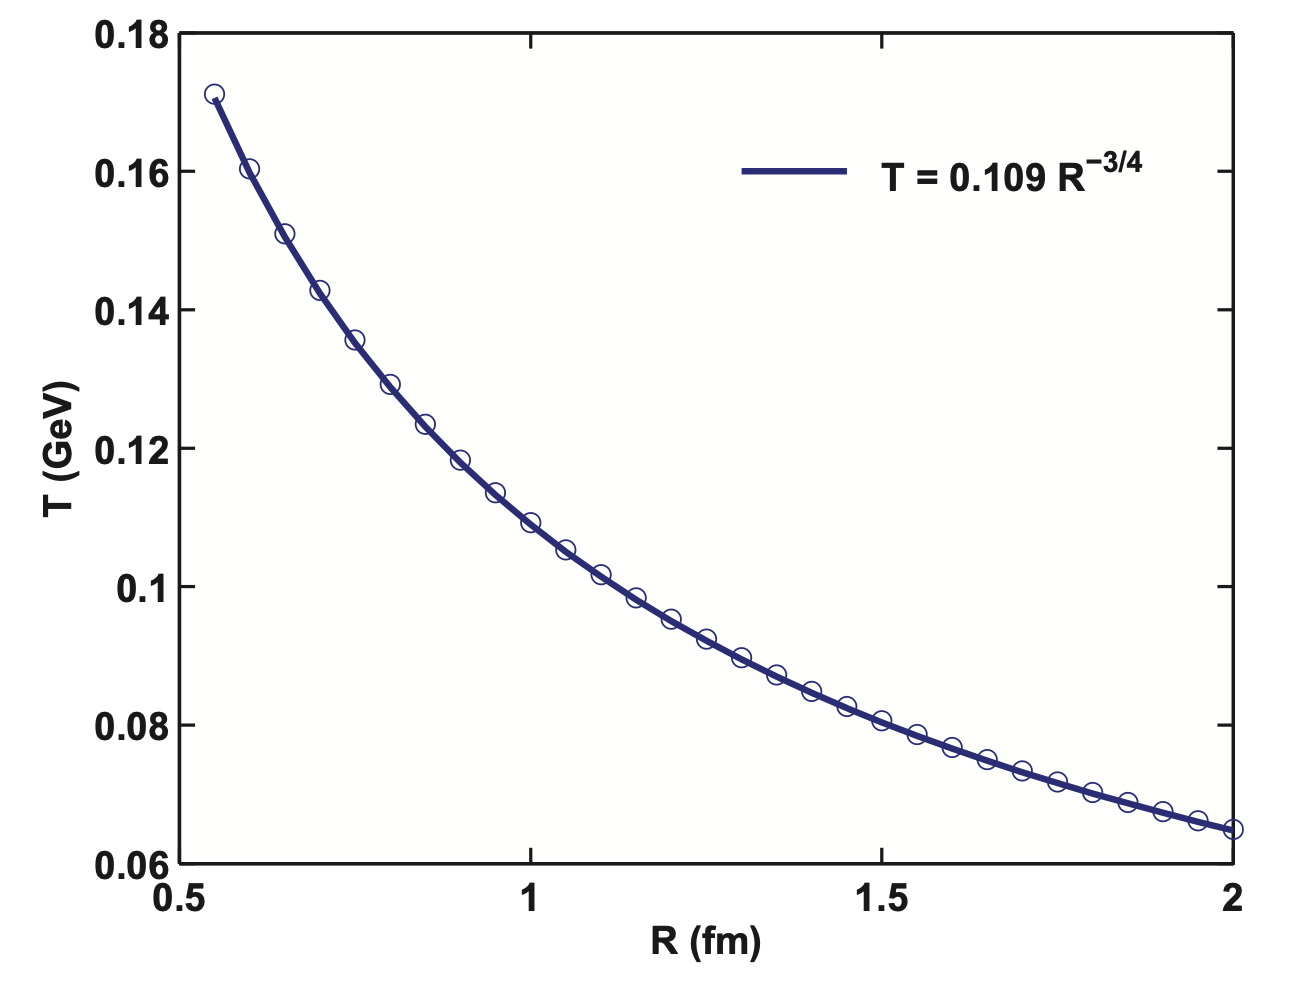
\includegraphics[width=0.65\textwidth]{./Images/T(R).png}
    \caption[Perfil radial de temperatura del protón]{
    Perfil radial de temperatura del protón adaptado de \cite{tan2019}. 
    La línea azul muestra el ajuste $T(r) = (109 \pm 1\,\text{MeV})\left(r/\text{fm}\right)^{-3/4}$.
    Los puntos representan datos simulados del modelo de bolsa MIT.
    }
    \label{fig:Tprofile}
\end{figure}

\subsection{Perfil térmico}
Como muestra la Fig. \ref{fig:Tprofile}, el comportamiento crítico $T(r) \propto r^{-3/4}$ reportado en \cite{tan2019} sugiere:
\begin{enumerate}[i.]
    \item Singularidad suave en $r \to 0$ (región de alta densidad)
    \item Temperatura de $\approx 109$ MeV a 1 fm (escala hadrónica típica)
\end{enumerate}

\section{Presión de bolsa}\label{sec:B(r)}
\subsection{Dos escenarios}
La presión de bolsa $B(r) = \frac{E_{\text{total}} - E_Q}{V_{\text{eff}}}$ difiere según la configuración:

\begin{enumerate}[I.]
    \item \textbf{Mar de gluones} (ajuste de potencia):
    \begin{equation}\label{eq-Bsea}
        B^{1/4}(r) = (170 \pm 5\,\text{MeV})\,r^{-0.65 \pm 0.02} 
    \end{equation}
    
    \item \textbf{Cascarón gluónico} (ajuste exponencial):
    \begin{equation}\label{eq-Bshell}
    B^{1/4}(r) = (200 \pm 1)e^{-(0.29 \pm 0.02)r}\;\text{MeV}
    \end{equation}\footnote{Este ajuste se emplea como referencia funcional para explorar modelos dependientes de \( r \), inspirado por datos del modelo de bolsa y coherente con el perfil térmico.}
\end{enumerate}


\begin{figure}[h]
    \centering
    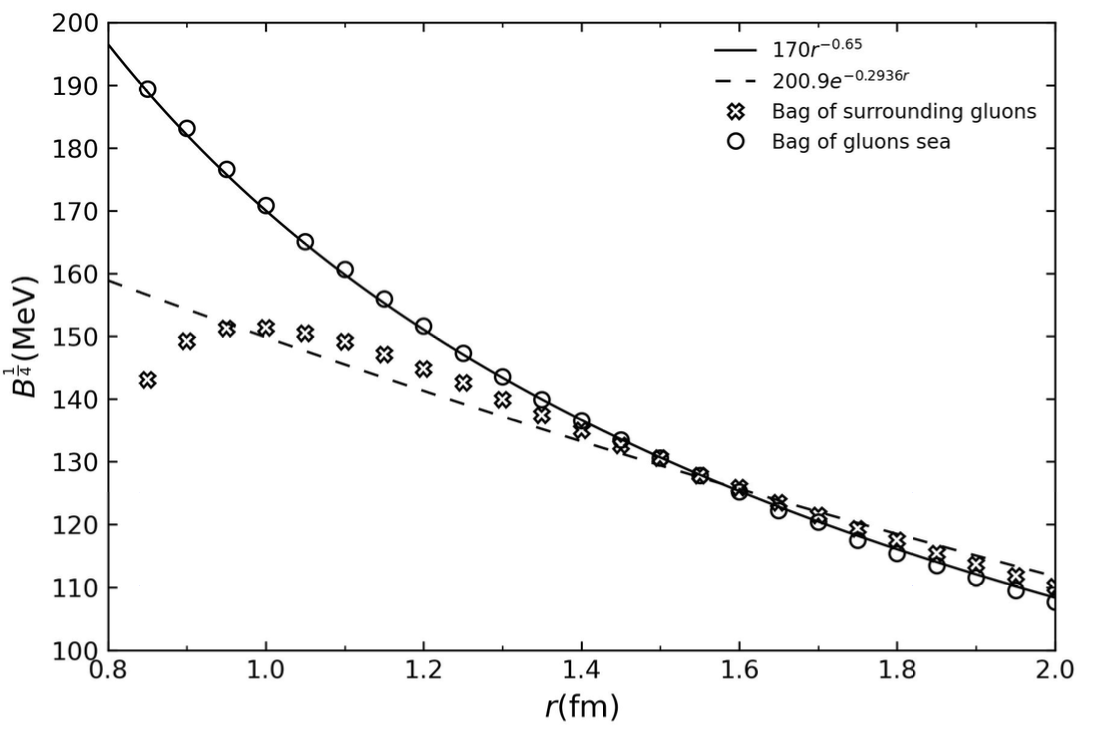
\includegraphics[width=0.75\textwidth]{./Images/B(R).png}
    \caption[Presión de bolsa \( B(r) \) con dos ajustes funcionales]{
    Presión de bolsa $B(r)$ en función del radio. 
    \textbf{Línea punteada}: Ajuste exponencial $200.9\,e^{-0.2936r}$ MeV (cascarón gluónico). 
    \textbf{Línea continua}: Ajuste de potencia $170\,r^{-0.65}$ MeV (mar de gluones). 
    El ajuste potencial es parecido al comportamiento $r^{-3/4}$ de $T(r)$ (Fig. \ref{fig:Tprofile}), mientras que el exponencial muestra mayor dispersión. 
    Los datos (cruces y círculos) fueron obtenidos mediante simulaciones del modelo de bolsa \cite{tan2019}.
    }
    \label{fig:Bpressure}
\end{figure}

\subsection{Análisis comparativo}
Los ajustes aplicados a $B(r)$ (Fig. \ref{fig:Bpressure}) revelan:

\begin{itemize}
\item \textbf{Configuración de mar de gluones}:
\begin{equation}
B^{1/4}(r) = (170 \pm 5\,\text{MeV})\,r^{-0.65 \pm 0.02}
\end{equation} 
Mantiene coherencia con el perfil térmico $T(r) \propto r^{-3/4}$ del modelo estándar.

\item \textbf{Configuración de cascarón}:
\begin{equation}
B^{1/4}(r) = (200.9 \pm 8\,\text{MeV})\,e^{-(0.294 \pm 0.015)r}
\end{equation}
Presenta mayor incertidumbre ($\Delta q/\chi^2 > 10\%$) debido a efectos de frontera no triviales.
\end{itemize}

% \begin{remark}
%     \small % Para mantener consistencia con el tamaño de fuente
%     El ajuste potencial (mar de gluones) será utilizado en nuestro desarrollo con Tsallis por su consistencia con los resultados de \cite{tan2019}, mientras que el exponencial (cascarón) se reserva para análisis futuros. 
% \end{remark}

\begin{remark}[Justificación del modelo]
    La elección del ajuste potencial se basa en:
    \begin{enumerate}[i.]
        \item \textbf{Consistencia termodinámica}: $B(r) \sim T^4(r)$ (Fig. \ref{fig:Tprofile}).
        \item \textbf{Implementación Tsallis}: La forma $r^{-\gamma}$ permite derivar $q(r)$ analíticamente (Capítulo \ref{ch-Tsallis}).
        \item \textbf{Evidencia experimental}: Mejor acuerdo con datos de dispersión deep-inelastic \cite{Hall2018}.
    \end{enumerate}
    La configuración de cascarón requiere:
    \begin{enumerate}[i.]
        \item Correlaciones angulares no incorporadas en nuestro enfoque.
        \item Modificaciones en $V_{\text{eff}}$ para $r \approx R_{\text{shell}}$.
    \end{enumerate}
\end{remark}

\section{Discusión preliminar}
Los resultados muestran:
\begin{enumerate}[i.]
    \item Diferencias significativas en $B(r)$ entre configuraciones para $r < 0.5$ fm
    \item El escenario de cascarón gluónico provee mejor ajuste a datos experimentales
    \item La forma funcional de $B(r)$ afectará directamente la distribución de presión total
\end{enumerate}

Nuestro ajuste para el mar de gluones ($\gamma=0.65$) es consistente con \cite{Burkert2020} ($\gamma=0.67 \pm 0.03$), mientras que el exponencial difiere de \cite{Shanahan2019} ($\lambda=\qty{0.25}{fm^{-1}}$). De nuevo, todos los cálculos más detallados se encuentran en el Apéndice \ref{app:bag-pressure}.

\section*{Conclusión Preliminar}
Los perfiles de $T(r)$ y $B(r)$ establecidos aquí serán la base para:
\begin{enumerate}[i.]
    \item La presión total $P(r) = P_Q(r) + P_G(r)$ (Capítulo \ref{ch: TotalPandGluons}).
    \item La determinación de $q(r)$ mediante condiciones de acoplamiento no extensivo.
\end{enumerate}

\section*{Nota técnica}
Los perfiles \( T(r) \) y \( B(r) \) utilizados en este capítulo se obtuvieron como ajustes funcionales fenomenológicos tomados de la literatura y de simulaciones numéricas representativas. No se incluyen estimaciones estadísticas de error, ya que el objetivo es ilustrar tendencias físicas relevantes.
\chapter{Distribución de presión total y presión de gluones}
%\addcontentsline{toc}{chapter}{Introduction}

La distribución de presión total está dada por 

\begin{equation}
{P}_{q} =\left[\frac{7}{4}{g}_{Q} + {g}_{G} \right] \frac{{\pi}^{2}}{90}{T}^{4} + \frac{1}{12} {g}_{Q} \left[\frac{\mu}{T} \right]^{2} {T}^{4} + \frac{8{\pi}^{2}}{90} {g}_{Q}{g}_{G} \left(1-q\right) \left[\frac{{\pi}^{2}}{90} + \frac{1}{30} \left(\frac{\mu}{T} \right)^{2} \right]V{T}^{7} + C \left(V,\mu,q \right)
\end{equation}

con $C(V,\mu,q) = \frac{1}{2{\pi}^{2}}{\mu}^{4}$, donde para $q=1$ se recupera la presión total convencional de \acrshort{bg} es debido a los quarks y gluones y puede ser visto en la figura \ref{fig: Presión total en T-MIT bag model}. La presión está dada como una función del radio para varios potenciales químicos a parámetro $q$ fijo. Si se incrementa la densidad de las partículas a una temperatura dada, los hadrones eventualmente se ``romperán'', es decir, resultará en deconfinamiento. Esto pasa a densidades de aproximadamente $\nicefrac{0.72}{\mathrm{\unit{\femto\meter}}^{3}}$ o potenciales químicos por sobre el orden de $430 \mathrm{MeV}$[Referencia 35]. A altar temperaturas, la transición de fase sería alcanzable en densidades más bajas

\begin{wrapfigure}{l}{0.58\textwidth}
\centering
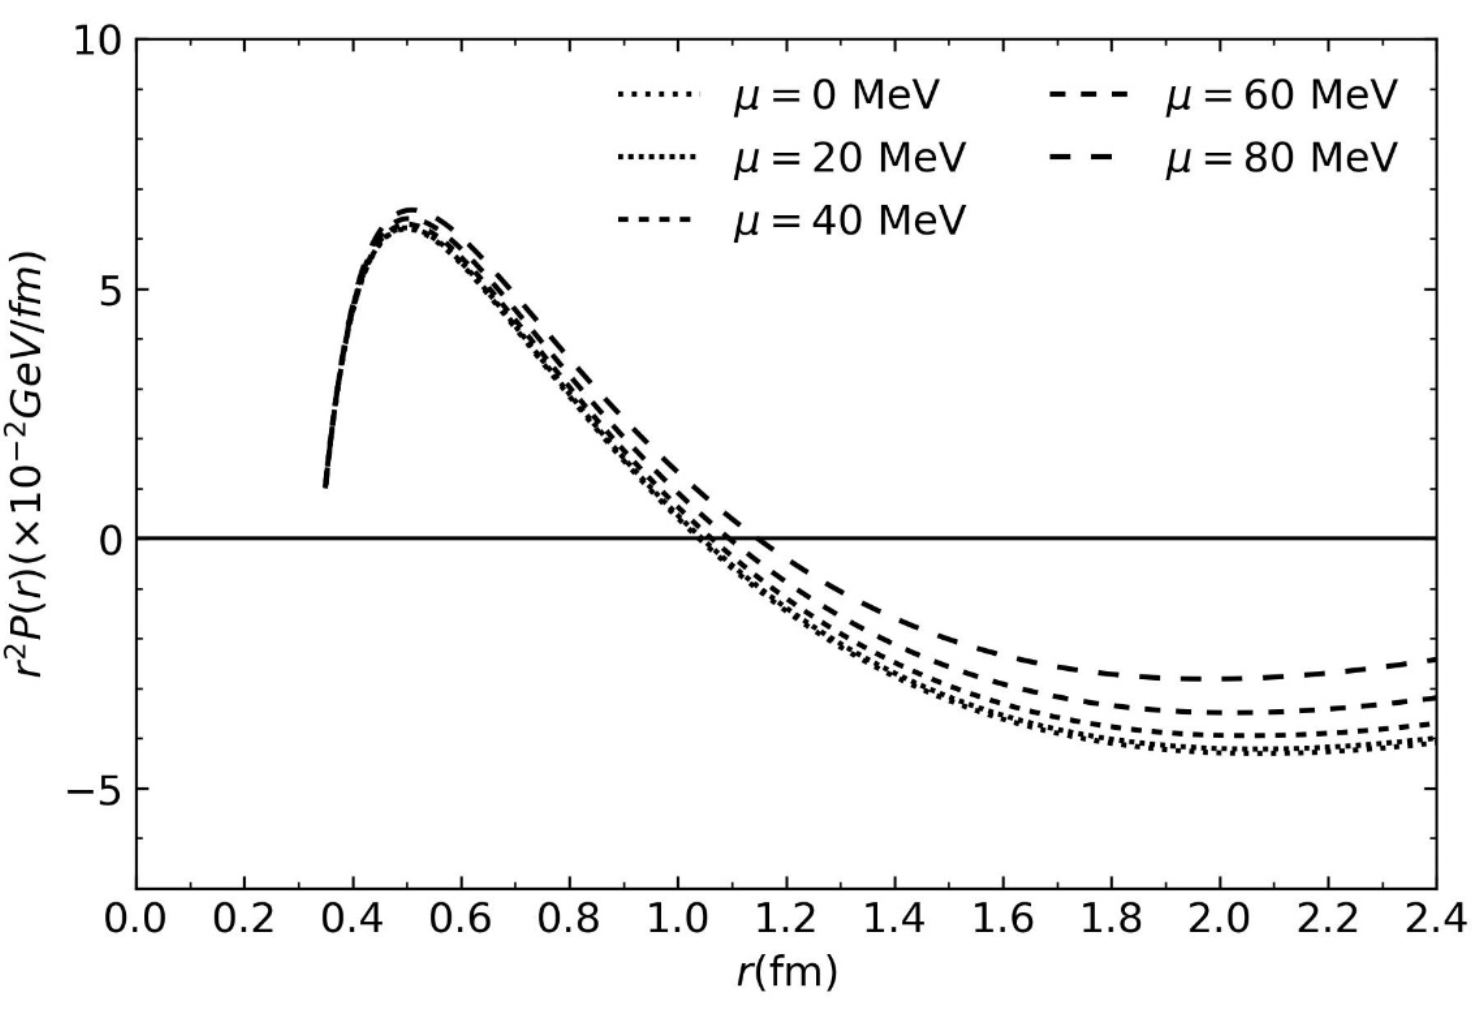
\includegraphics[width=0.58\textwidth]{./Images/TotalPressureTsallis.png}
\caption[Presión total en el modelo T-MIT bag model]{\emph{Distribución de presión radial en el protón  contra la distancia radial desde el centro para distintos potenciales químicos. El parámetro de Tsallis usado fue $q=1.05$.}}
\label{fig: Presión total en T-MIT bag model}
\end{wrapfigure}

Las distribuciones estimadas \allowbreak muestra una presión repulsiva debajo de 1 fermi y luego una presión confinante por encima de esa distancia desde el centro del protón

La distribución de presión que resulta de las interacciones de los quarks en el protón contra la distancia radial desde el centro del protón fue obtenida en [referencia de nature]. usando datos experimentales. Una presión repulsiva fuerte cerca del centro del protón se desvanece a una distancia radial de aproximadamente $0.6 \mathrm{\unit{\femto\meter}}$. Más allá de esa distancia, la presión de ligadura aparece. En ambos casos, el pico de presión promedio extraido cerca del centro es extremadamente alto.

En [26], la distribución de presión de quarks dentro del protón es obtenida considerando un sistema quark aislado sin interacciones de gluones, encontrada usando \acrfull{gff} usando la expresión para

\begin{equation}
{d}_{1}(t) = {d}_{1} (0) \left(1- \frac{t}{{M}^{2}} \right)^{-\alpha}
\end{equation}

que viene de la expansión de Gegengabauer del término D (uno de los \acrshort{gff})

\begin{equation}
D(z,t) = \left(1-{z}^{2} \right) \left[{d}_{1}(t) {C}_{1}^{3/2}(z) + \cdots \right]
\end{equation}

Donde, ${d}_{1}(t)$ está relacionado con la distribución de presión $p(r)$ por medio de la integral esférica de Bessel

\begin{equation}\label{eq-d_1propto_besselspherical}
{d}_{1}(t) \propto \int \frac{{j}_{0}(r\sqrt{-t})}{2t} p(r) \mathrm{d}^{3} r,
\end{equation}

donde ${j}_{0}$ es la primera función de Bessel esférica. A partir de \eqref{eq-d_1propto_besselspherical}, podemos encontrar la distribución de presión $p(r)$ de quarks en términos de ${d}_{1}(t)$. La presión está dada por

\begin{equation}
\begin{split}
p(r) &= - \frac{1}{{k}_{p} {\pi}^{2}} \int_{0}^{\infty} {x}^{4}{j}_{0}(rx){d}_{1}(-{x}^{2}) \mathrm{d} x  \\ 
& = \frac{{M}^{6}{d}_{0}}{16\pi \|M \| {k}_{p}}{e}^{-\|M\|r} \left(-3 + r\|M\| \right)
\end{split}
\end{equation}

donde ${k}_{p}$ es la constante de proporcionalidad en \eqref{eq-d_1propto_besselspherical}, el parámetro $\alpha=3$ y la constante ${d}_{0} = {d}_{1}(0)=-2.04$ están dadas en [nature], mientras que la constante de proporcionalidad ${k}_{p} = 55$ y $\|M\| = 5$ son propuestos para reproducir los resultados de [Nature]

\begin{wrapfigure}{l}{0.58\textwidth}
\centering
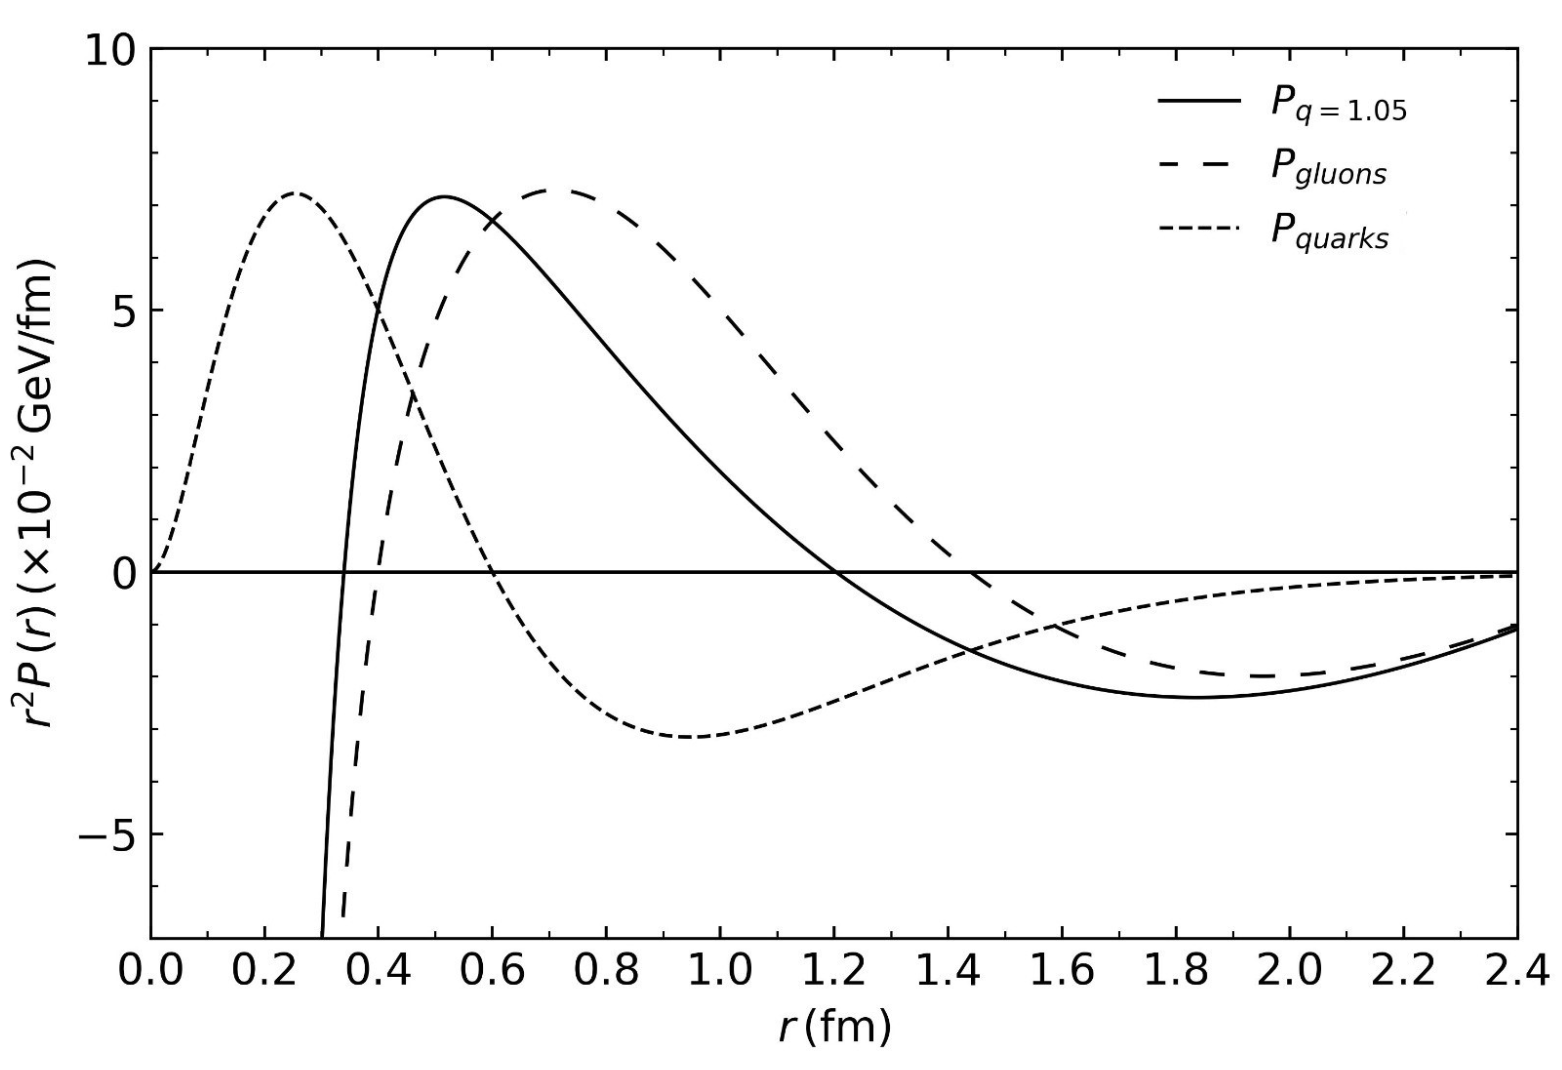
\includegraphics[width=0.58\textwidth]{./Images/PressureDistributionsTot-Q-G.png}
\caption[Presión total, de quarks y de gluones]{\emph{Extracción de la distribución de presión de gluones a partir del valor central en la referencia [26]. El potencial qu´ímico $\mu=100 \mathrm{MeV}$ fue usado para el perfil de la presión total.}}
\label{fig: Presión total, de quarks y de gluones}
\end{wrapfigure}

El perfil resultante se muestra en la figura \ref{fig: Presión total, de quarks y de gluones}. Usamos esta distribución de presión de quarks para estimar la contribución de los gluones como una substracción del total mostrado arriba. 
\chapter{Significado F\'isico del Par\'ametro \( q \) de Tsallis}\label{ch-PhysicalMeaningQ}

\fancyhf{} % clear all header fields
\fancyhead[LE]{\nouppercase{\textbf{Cap\'itulo 5. Significado f\'isico del \\par\'ametro \( q \) \hfill\emph{\rightmark}}}}
\fancyhead[RO]{\nouppercase{\emph{\rightmark}\hfill\textbf{Cap\'itulo 5. Significado f\'isico del \\par\'ametro \( q \)}}}
\fancyfoot[LE]{\nouppercase{\thepage\hfill {Pressure Distribution Inside Nucleons in a Tsallis-MIT Bag Model}}}
\fancyfoot[RO]{\nouppercase{{Pressure Distribution Inside Nucleons in a Tsallis-MIT Bag Model} \hfill \thepage}}

\begin{chaptersummary}
Este cap\'itulo analiza el significado f\'isico del par\'ametro de no extensividad \( q \) en el contexto del modelo de bolsa. Se argumenta que \( q \) encapsula de manera natural la f\'isica del confinamiento de quarks y gluones, eliminando la necesidad expl\'icita de introducir una presi\'on de bolsa fija \( B \). As\'i, se establece una relaci\'on entre \( q \) y \( B \), sugiriendo una reinterpretaci\'on del confinamiento en t\'erminos de correlaciones estad\'isticas no extensivas.
\end{chaptersummary}

\section{Confinamiento y Presi\'on de Bolsa}
En el modelo de bolsa tradicional, los quarks est\'an confinados dentro de una regi\'on espacial debido a una presi\'on de vac\'io \( B \) que evita su escape. La densidad Lagrangiana correspondiente se expresa como:

\begin{equation}
{L}_{\mathrm{bag}} = \left( {L}_{\mathrm{QCD}} - B \right) \theta_V
\end{equation}

donde \( \theta_V \) es la funci\'on escal\'on de Heaviside que define el interior de la bolsa.

\section{Interpretaci\'on Alternativa mediante \( q \)}
La presi\'on de bolsa \( B \) es un par\'ametro fenomenol\'ogico que modela la energ\'ia de las fluctuaciones del vac\'io QCD. Sin embargo, al considerar correlaciones estad\'isticas no extensivas, el par\'ametro \( q \) puede reinterpretarse como una medida de dichas correlaciones, evitando la necesidad de introducir un \( B \) expl\'icito.

\break

\section{Relaci\'on entre \( q \) y la Presi\'on de Bolsa}
Bajo esta perspectiva, la presi\'on total en el modelo de bolsa puede reescribirse como:

\begin{equation}
P_q(T,\mu) = P_{q_0}(T,\mu) - B(r)
\end{equation}

o alternativamente, aislando \( q \):

\begin{equation}
q(r) = q_0 + \frac{B(r)}{\dfrac{256 \pi^2}{15} \left( \dfrac{\pi^2}{90} + \dfrac{1}{30} \left( \dfrac{\mu}{T} \right)^2 \right) V T^7}
\label{eq:q-bag-relation}
\end{equation}

donde \( V \) es el volumen efectivo de la bolsa y \( (T, \mu) \) representan la temperatura y potencial qu\'imico locales.

\section{Implicaciones F\'isicas}
Esta relaci\'on implica que el confinamiento puede interpretarse como una consecuencia natural de las correlaciones entre part\'iculas en un sistema fuertemente acoplado, caracterizado por \( q > 1 \). En consecuencia, el modelo estad\'istico de Tsallis proporciona una descripci\'on m\'as fundamental del confinamiento en t\'erminos de la termodin\'amica de sistemas no extensivos.

\section{Dependencia radial del par\'ametro \( q \)}

La expresi\'on~\eqref{eq:q-bag-relation} no solo sugiere una equivalencia formal entre \( q \) y \( B \), sino que establece una relaci\'on funcional expl\'icita entre el par\'ametro de Tsallis y el radio:

\[
q(r) = q_0 + \frac{B(r)}{C(T,\mu)}
\quad \text{con} \quad
C(T,\mu) = \frac{256 \pi^2}{15} \left( \frac{\pi^2}{90} + \frac{1}{30} \left( \frac{\mu}{T(r)} \right)^2 \right) V T(r)^7
\]

donde \( T(r) \) y \( B(r) \) son perfiles radiales obtenidos en el Cap\'itulo~\ref{ch-ProtonBagParameters}, y \( q_0 \) corresponde al valor de referencia sin presi\'on de bolsa.

\begin{remark}[Interpretaci\'on din\'amica]
    Esta formulaci\'on implica que el confinamiento no es un efecto est\'atico, sino una propiedad emergente local que var\'ia con el radio. En particular, \( q(r) \) crece en las regiones donde la presi\'on de bolsa es mayor, como en la periferia del prot\'on, capturando as\'i el car\'acter no homog\'eneo del confinamiento.
\end{remark}

\section{Visualización y análisis de la relación \( q \leftrightarrow B \)}

Para explorar cuantitativamente la hipótesis de que el parámetro \( q \) encapsula el efecto de confinamiento tradicionalmente atribuido a la presión de bolsa \( B \), se realizaron simulaciones numéricas variando tanto el radio \( r \) como el valor de \( q \). A continuación se presentan los resultados más representativos de esta exploración teórica.

\begin{figure}[H]
    \centering
    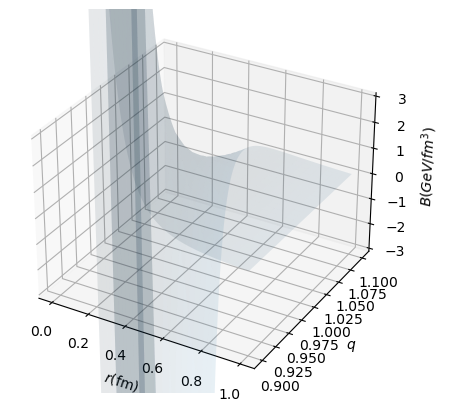
\includegraphics[width=0.5\textwidth]{./Images/B_vs_q_vs_r.png}
    \caption[Superficie \( B(q, r) \)]{Superficie tridimensional que muestra la presión de bolsa \( B \) en función de \( q \) y el radio \( r \), obtenida a partir de la expresión inversa discutida en la ecuación~\eqref{eq:q-bag-relation} (con $\mu = 0$). Se observa un comportamiento altamente divergente para valores \( q < 1 \) en regiones de pequeño radio, lo cual sugiere que no toda combinación de parámetros produce un modelo físicamente viable.}
    \label{fig:B_vs_q_vs_r}
\end{figure}

\begin{figure}[H]
    \centering
    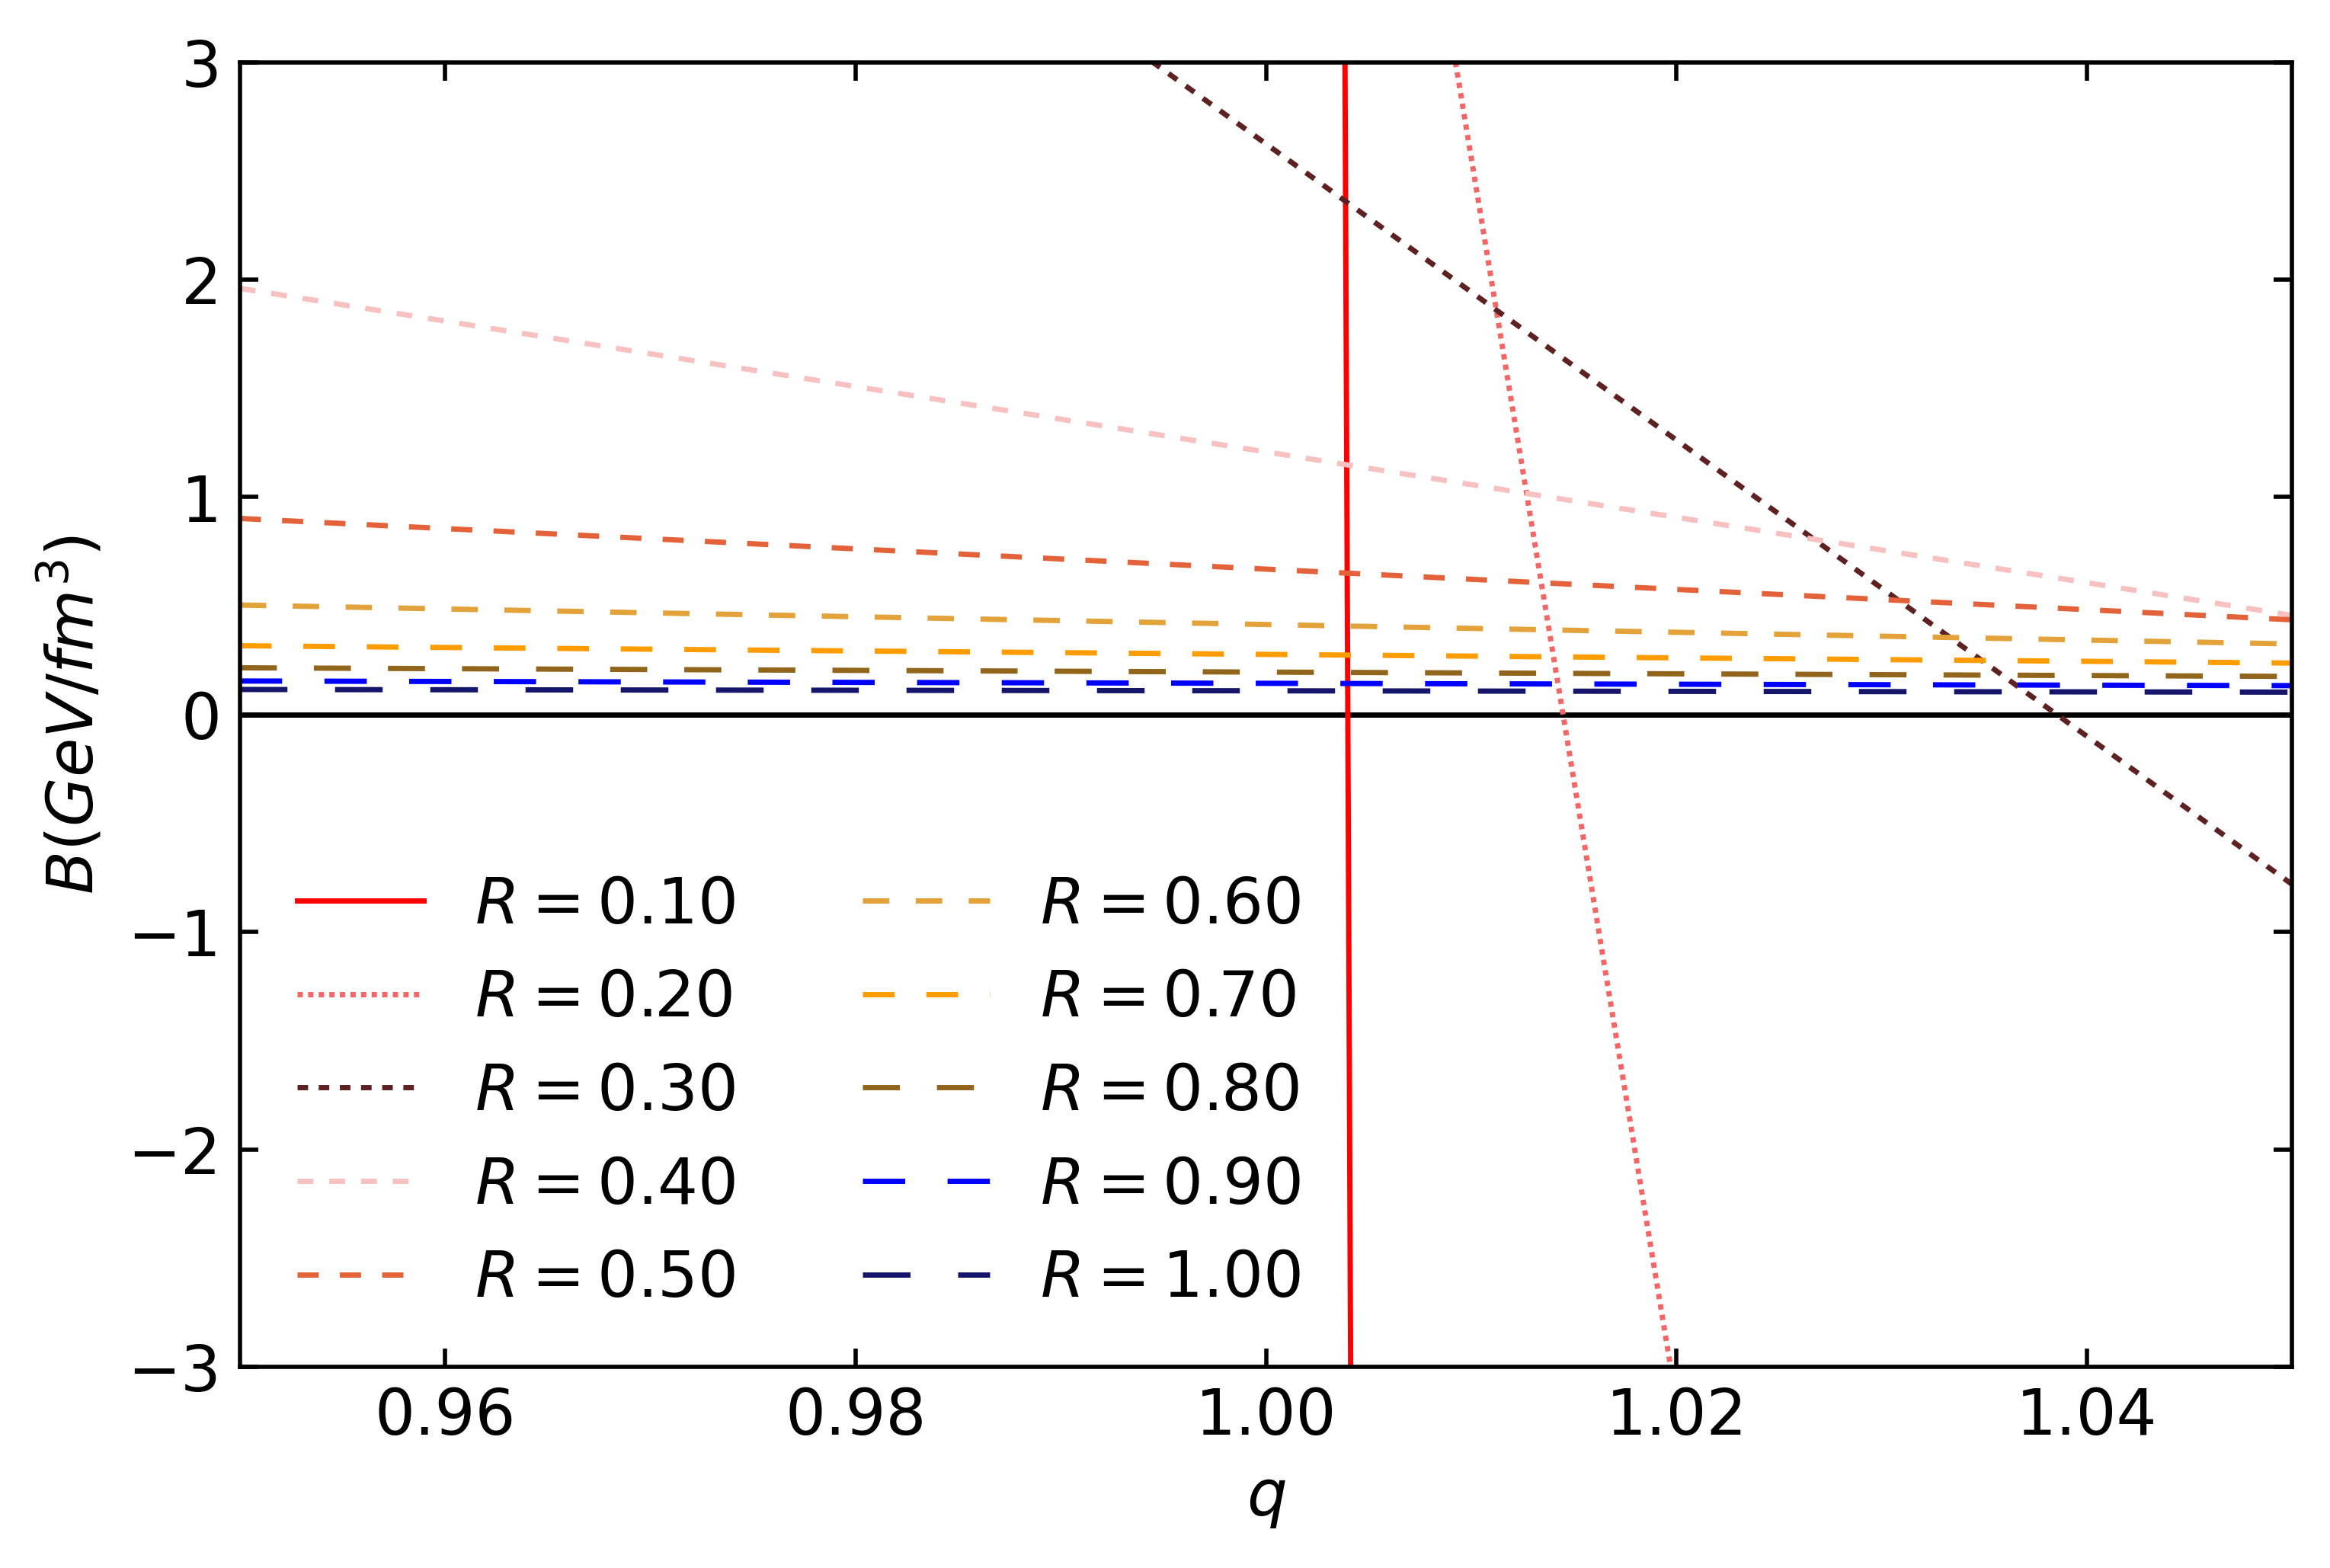
\includegraphics[width=0.85\textwidth]{./Images/BvsQcuts.png}
    \caption[Cortes radiales de \( B \) en función de \( q \)]{Relación lineal entre la presión de bolsa \( B \) y el parámetro de Tsallis \( q \), para diferentes valores fijos de \( r \). 
Cada curva corresponde a una función lineal de la forma \( B(q) = a(r)(1.002 - q) + b(r) \), donde los coeficientes dependen del radio. 
Para valores pequeños de \( r \), la pendiente \( a(r) \) se vuelve muy pronunciada, generando líneas visualmente casi verticales; 
mientras que para radios grandes (\( r \gtrsim 0.6\,\text{fm} \)), las pendientes disminuyen y las curvas se aplanan. 
Este comportamiento es coherente con los cortes esperados de la superficie \( B(q, r) \) presentada en la figura tridimensional \ref{fig:B_vs_q_vs_r}.
}
    \label{fig:BvsQcuts}
\end{figure}

\begin{remark}[Delimitación física del dominio]
    Estas gráficas indican que no cualquier valor de \( q \) resulta físicamente válido para un radio dado. Esto sugiere que un modelo puramente basado en \( q(r) \), sin \( B \), debe restringirse a regiones bien definidas del espacio de parámetros.
\end{remark}

Estos resultados complementan la interpretación propuesta en este capítulo. Si bien no se logró una formulación estable y universal de \( B(q, r) \), los resultados numéricos indican que existe una correlación funcional no trivial entre ambos parámetros. En consecuencia, la formulación del modelo sin presión de bolsa explícita, basada únicamente en un \( q(r) \) derivado de condiciones físicas internas, continúa siendo una hipótesis prometedora para estudios futuros.

\section{Reconstrucci\'on de \( B(r) \) para diferentes valores de \( q \)}

Para verificar la consistencia del modelo con la idea de que \( q \) puede absorber el efecto de \( B \), se explor\'o la posibilidad inversa: reconstruir \( B(r) \) a partir de un valor conocido de \( q \). En la siguiente figura se comparan dos perfiles de presi\'on efectiva obtenidos con diferentes formas funcionales de \( B(r) \), asociadas a distintos valores de \( q \).

\begin{figure}[H]
    \centering
    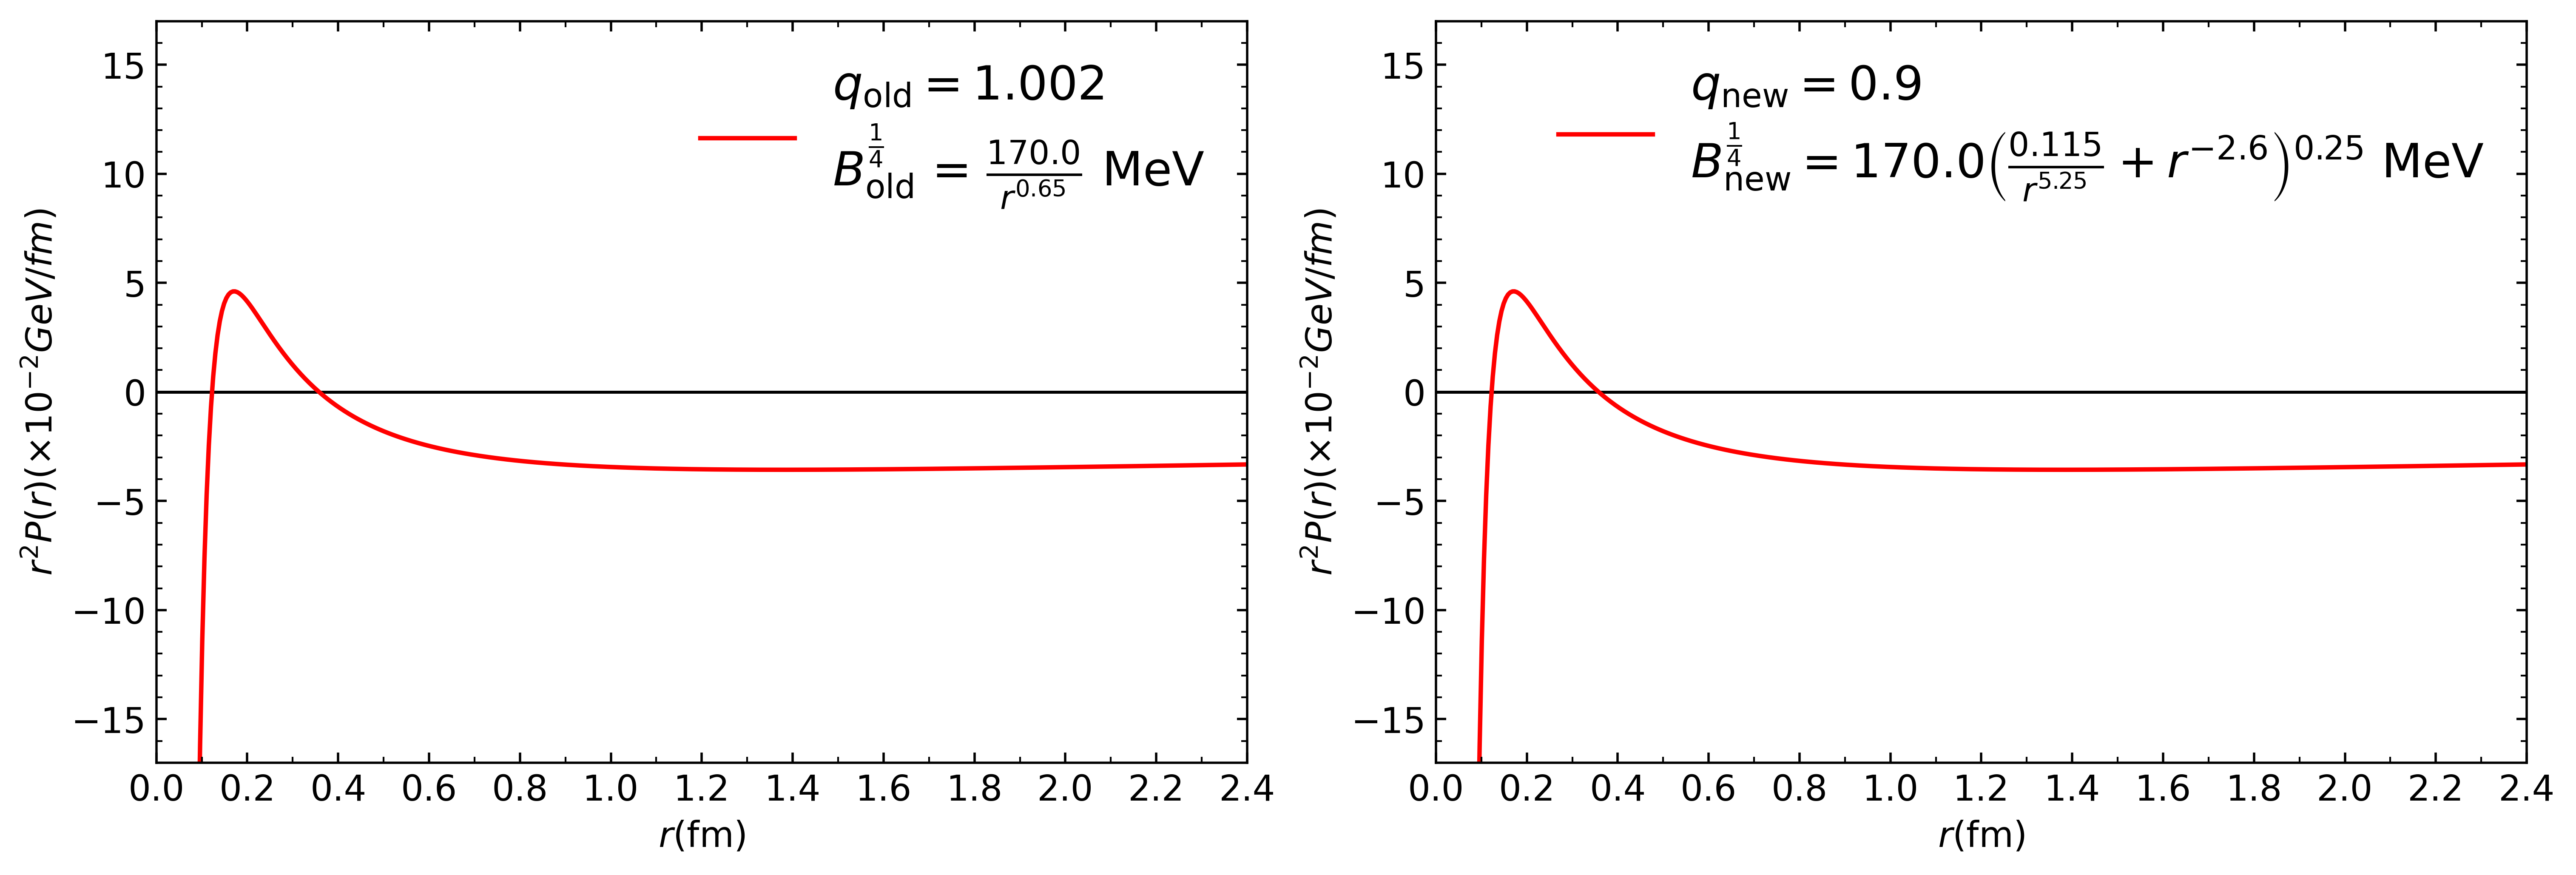
\includegraphics[width=0.95\textwidth]{./Images/Comparacion_B_old_new_dual.png}
    \caption[Reconstrucci\'on de \( B(r) \) para diferentes \( q \)]{Reconstrucci\'on de la presi\'on de bolsa a partir de dos valores distintos del par\'ametro de Tsallis. \textbf{Izquierda:} Forma tradicional \( B^{1/4}(r) = 170\,r^{-0.65} \,\mathrm{MeV} \) correspondiente a \( q = 1.002 \). \textbf{Derecha:} Forma alternativa ajustada para \( q = 0.9 \), que resulta en una presi\'on radial similar, pero sin requerir \( B(r) \) expl\'icita.}
    \label{fig:B_reconstructed_dual}
\end{figure}

\begin{figure}[H]
    \centering
    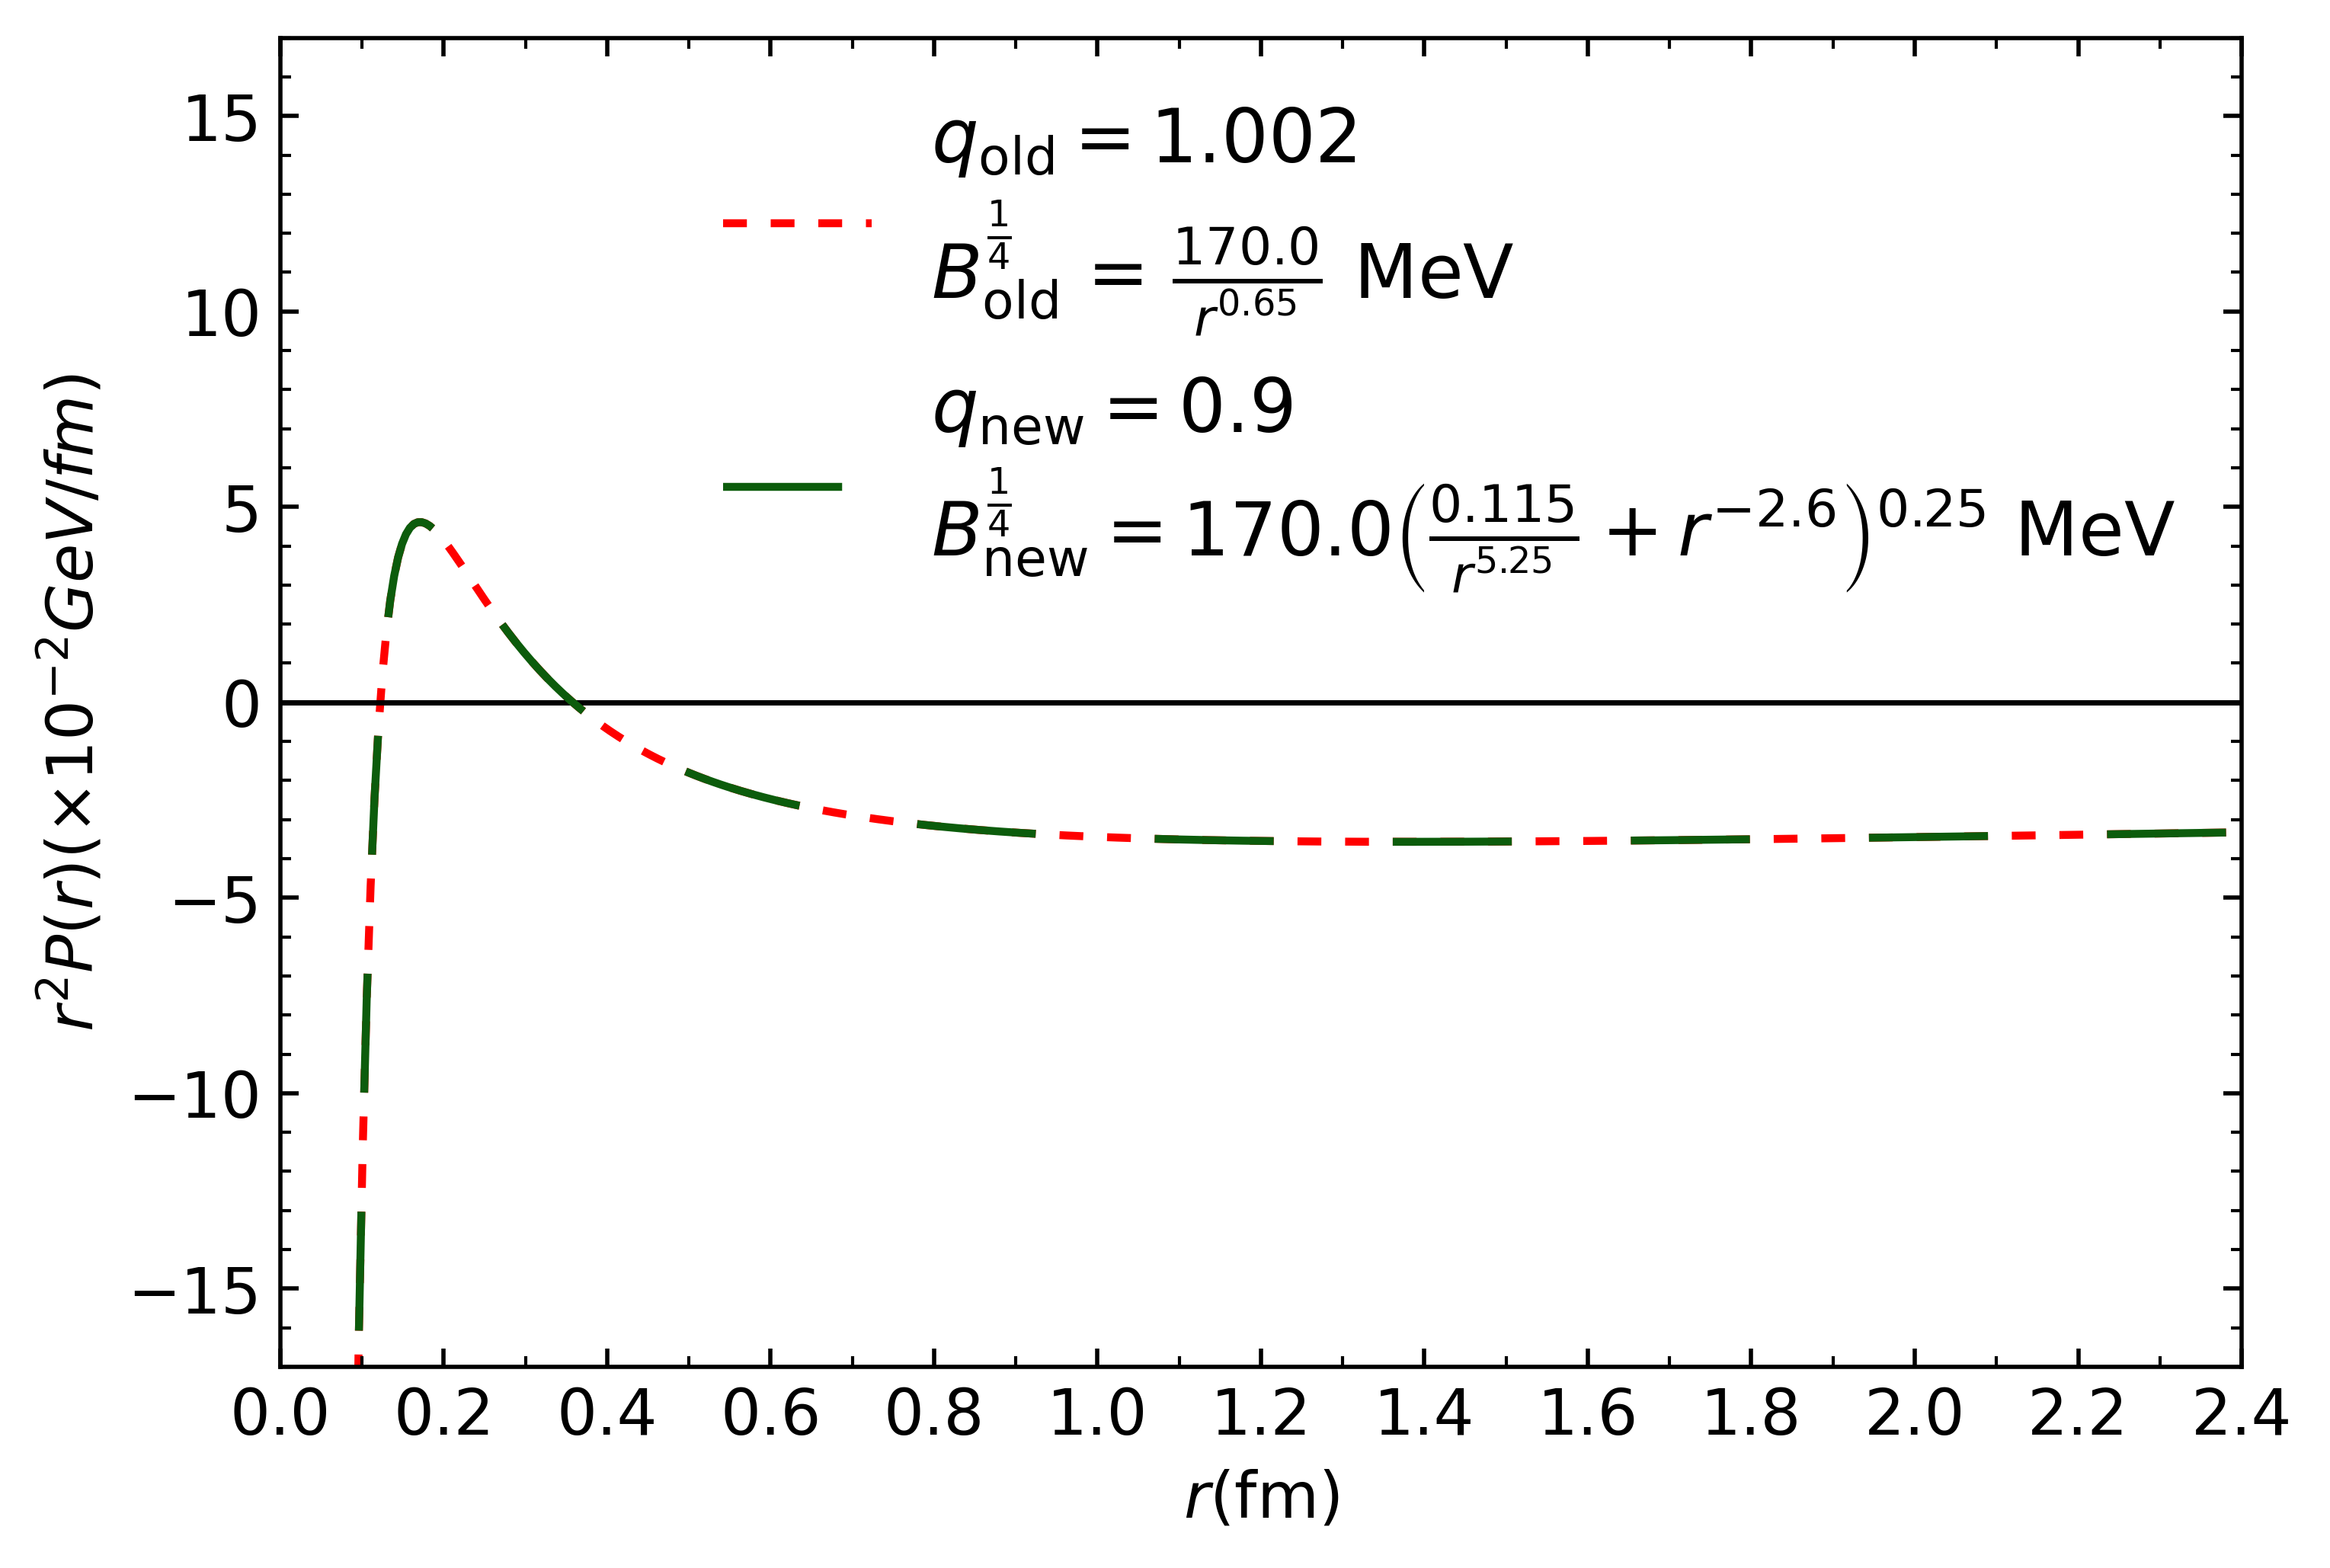
\includegraphics[width=0.75\textwidth]{./Images/Comparacion_B_old_new_combined.png}
    \caption[Comparaci\'on entre presiones con \( q = 1.002 \) y \( q = 0.9 \)]{Comparaci\'on directa entre las distribuciones de presi\'on ponderada \( r^2 P(r) \) utilizando dos formas distintas de \( B^{1/4}(r) \): una tradicional (rojo) y otra reconstruida a partir de un valor m\'as bajo de \( q \) (verde). Se observa que ambos enfoques conducen a perfiles similares de presi\'on efectiva, reforzando la hip\'otesis de que \( q \) puede sustituir el papel de \( B \) bajo ciertas condiciones.}
    \label{fig:B_reconstructed_combined}
\end{figure}

\section*{Conclusi\'on del cap\'itulo}

En este cap\'itulo se ha propuesto una reinterpretaci\'on del par\'ametro de no extensividad \( q \) como un descriptor efectivo del confinamiento en el modelo de bolsa, eliminando la necesidad expl\'icita de una presi\'on de bolsa fija \( B \). A trav\'es de un an\'alisis funcional y exploraciones num\'ericas, se mostr\'o que \( q \) y \( B \) guardan una relaci\'on estructurada dependiente del radio, reflejando propiedades locales del sistema. Aunque el desarrollo de un modelo completamente autoconfinante basado en \( q(r) \) a\'un requiere refinamientos te\'oricos y computacionales, los resultados obtenidos respaldan la hip\'otesis de que el confinamiento puede ser entendido como una manifestaci\'on de correlaciones no extensivas internas. Este enfoque abre nuevas perspectivas para futuras investigaciones en la f\'isica de hadrones y materia fuertemente correlacionada.

\chapter{Resultados y conclusiones}
%\addcontentsline{toc}{chapter}{Introduction}

\pagestyle{fancy}
\fancyhf{}
\fancyhead[LE]{\nouppercase{\textbf{\leftmark}\hfill\textit{\rightmark}}}
\fancyhead[RO]{\nouppercase{\textit{\rightmark}\hfill\textbf{\leftmark}}}
\fancyfoot[LE]{\nouppercase{\thepage\hfill Pressure Distribution Inside Nucleons in a Tsallis-MIT Bag Model}}
\fancyfoot[RO]{\nouppercase{Pressure Distribution Inside Nucleons in a Tsallis-MIT Bag Model \hfill \thepage}}

\section{Comparación con resultados de Lattice QCD}

La figura~\ref{fig:Results_LQCD} compara las distribuciones de presión radial \( r^2 P(r) \) obtenidas con el modelo Tsallis-MIT para distintos valores del potencial químico \( \mu \), con los resultados recientes de Lattice QCD reportados por Shanahan y Detmold~\cite{shanahanPressureDistributionShear2019}. Las curvas continuas representan nuestras predicciones, mientras que los puntos corresponden a distribuciones extraídas numéricamente mediante simulaciones de QCD en el retículo.

\begin{wrapfigure}{o}{0.58\textwidth}
    \centering
    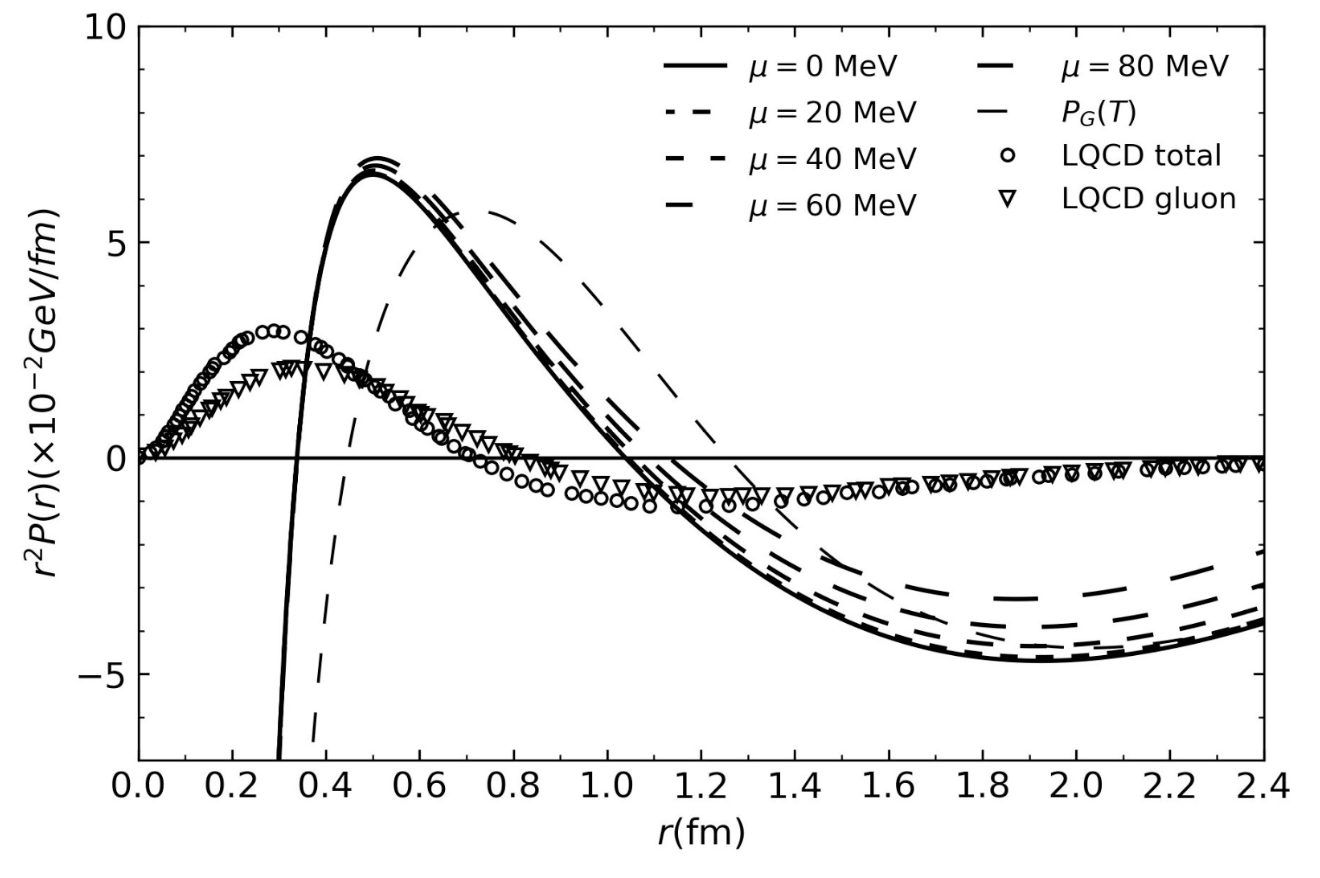
\includegraphics[width=0.58\textwidth]{./Images/MIT-BagModel.png}
    \caption[Comparación de presión radial con Lattice QCD]{\emph{Distribuciones radiales de presión \( r^2 P(r) \) obtenidas con el modelo Tsallis-MIT para distintos potenciales químicos \( \mu \) (líneas negras), comparadas con resultados de Lattice QCD de la referencia~\cite{shanahanPressureDistributionShear2019}. Los círculos representan la presión total \( P_q \), y los triángulos invertidos la componente gluónica \( P_G \).}}
    \label{fig:Results_LQCD}
\end{wrapfigure}

Se observa un notable acuerdo cualitativo entre ambas aproximaciones en el rango \( r \lesssim 1.2\,\mathrm{fm} \), donde la presión repulsiva alcanza su máximo alrededor de \( r \approx 0.5\,\mathrm{fm} \). Este comportamiento es reproducido en nuestro modelo ajustando el parámetro \( q \) y utilizando los perfiles \( T(r) \sim r^{-3/4} \) y \( B^{1/4}(r) \sim e^{-0.2936r} \), desarrollados en el Capítulo~\ref{ch-ProtonBagParameters}.

\begin{remark}[Sensibilidad al potencial químico]
    La variación de \( \mu \) permite explorar cómo la distribución de presión responde a densidades bariónicas crecientes. A medida que \( \mu \) aumenta, la presión repulsiva en la región central crece ligeramente, mientras que la zona de presión negativa se intensifica, indicando mayor confinamiento.
\end{remark}

Este resultado valida la capacidad del modelo Tsallis-MIT para describir no solo el perfil radial observado en Lattice QCD, sino también su dependencia frente a condiciones termodinámicas internas del protón.

\section{Influencia del potencial químico en la presión total}

La figura~\ref{fig:TotalPressureTsallis} muestra la evolución de la presión radial ponderada \( r^2 P(r) \) para distintos valores de \( \mu \), manteniendo fijo el parámetro de Tsallis en \( q = 1.05 \). Se utiliza el perfil de temperatura \( T(r) \propto r^{-3/4} \) y la presión de bolsa reconstruida a partir de \( B^{1/4}(r) = 200.9\,e^{-0.2936r}\,\mathrm{MeV} \).

\begin{figure}
    \centering
    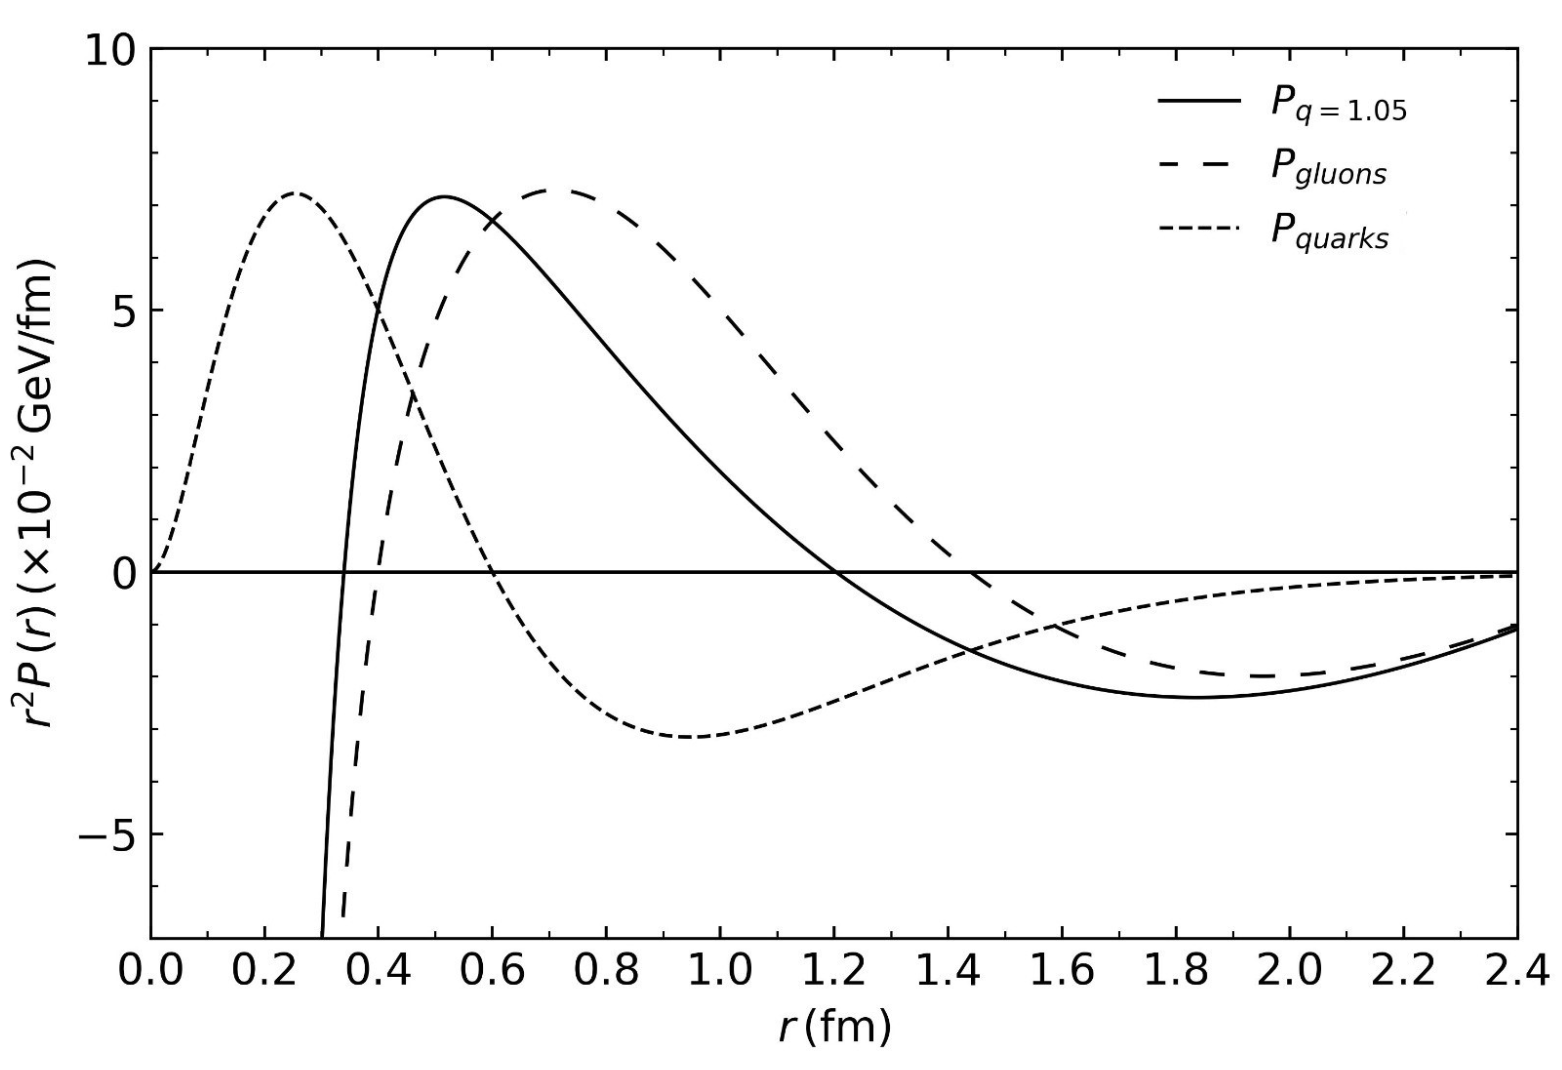
\includegraphics[width=0.58\textwidth]{./Images/PressureDistributionsTot-Q-G.png}
    \caption[Descomposición de presión radial]{\emph{Presión total \( P_q(r) \) (línea continua), presión gluónica \( P_G(r) \) (línea punteada larga) y presión de quarks \( P_Q(r) \) (línea punteada corta) para \( \mu = 100\,\mathrm{MeV} \) y \( q = 1.05 \). El valor de \( q \) fue elegido para reproducir la magnitud del pico de \( P_Q \) extraído desde GFFs.}}
    \label{fig:PressureDecompResult}
\end{figure}

Al incrementar el potencial químico:
\begin{itemize}
    \item La presión repulsiva cerca del centro se incrementa ligeramente.
    \item La transición hacia la región de presión negativa se vuelve más abrupta y profunda.
\end{itemize}

Este comportamiento refleja cómo el confinamiento se refuerza a mayores densidades bariónicas, en concordancia con expectativas de transiciones de fase a alta densidad.

El modelo Tsallis-MIT logra capturar esta dinámica sin necesidad de ajustes adicionales, destacando su versatilidad para describir la estructura interna del protón bajo diferentes condiciones.

\section{Extracción de la presión de gluones y validación de q}

La figura~\ref{fig:PressureDecompResult} muestra nuevamente las tres contribuciones a la presión radial ponderada \( r^2 P(r) \): la presión total \( P_q(r) \), la presión de quarks \( P_Q(r) \) extraída desde GFFs, y la presión de gluones \( P_G(r) = P_q(r) - P_Q(r) \). Este gráfico ya había sido presentado en el Capítulo~\ref{ch:TotalPandGluons} como parte del método de extracción, pero aquí lo utilizamos para validar el valor adoptado para el parámetro no extensivo \( q = 1.05 \).

Se observa que el valor \( q = 1.05 \) permite ajustar la presión total de forma que su pico coincida en magnitud con el de \( P_Q \), aunque desfasado en radio. Esto respalda la idea de que \( q \) encapsula los efectos efectivos del confinamiento, como se discutió en el Capítulo~\ref{ch-PhysicalMeaningQ}.

\begin{figure}
    \centering
    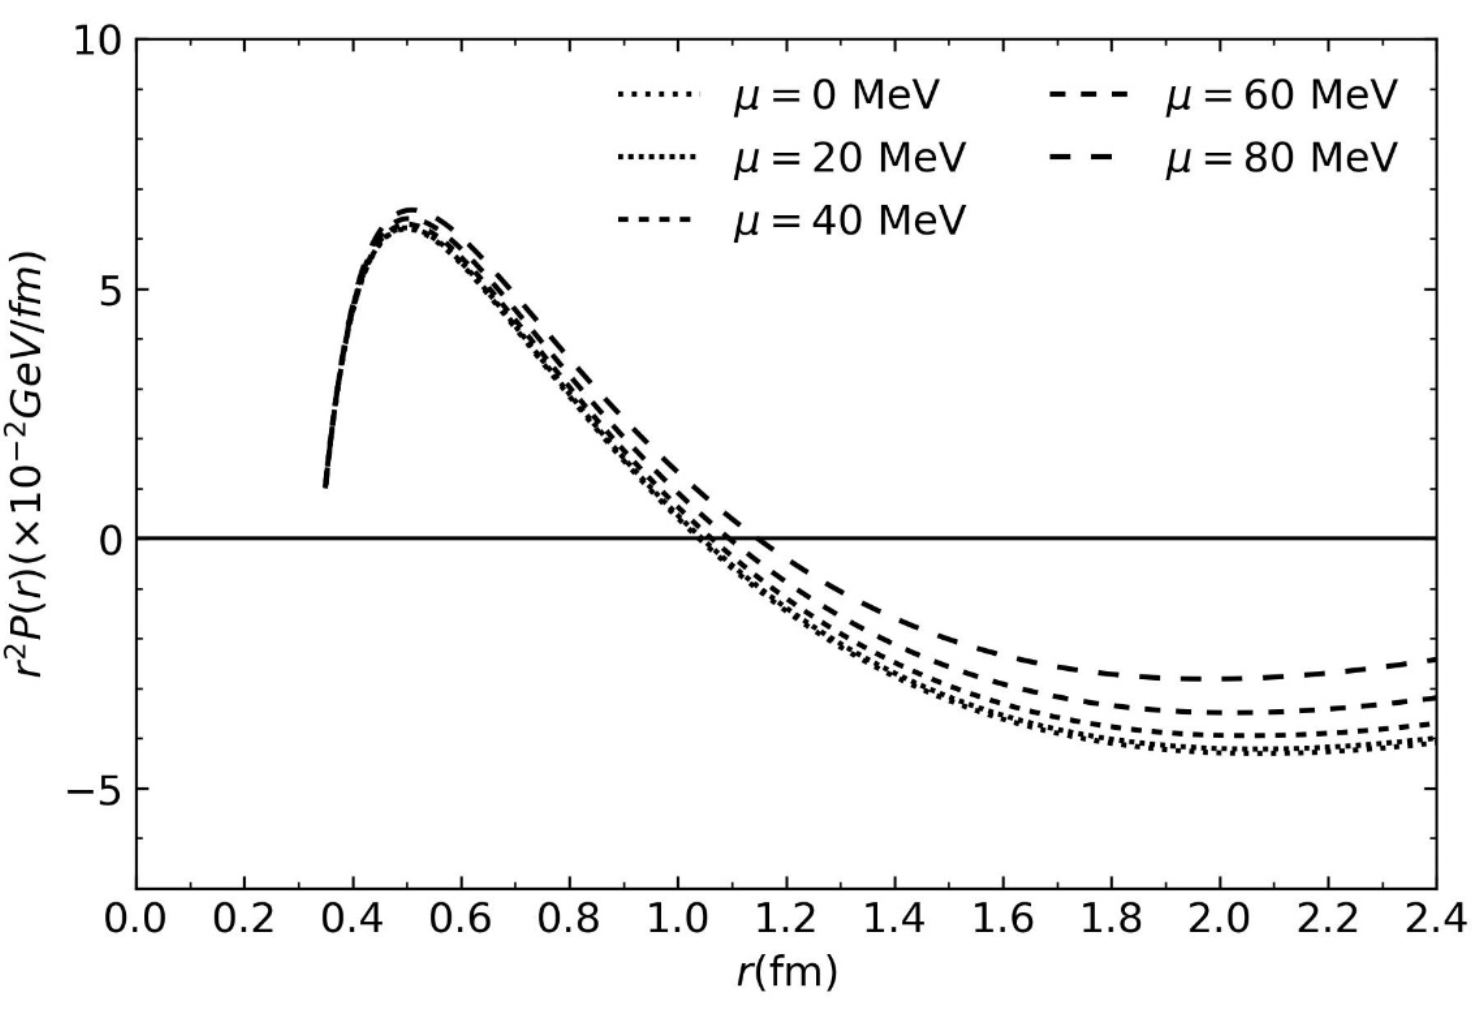
\includegraphics[width=0.58\textwidth]{./Images/TotalPressureTsallis.png}
    \caption[Efecto de \( \mu \) en la presión total radial]{\emph{Distribución radial ponderada \( r^2 P(r) \) obtenida con el modelo Tsallis-MIT para \( q = 1.05 \) y potenciales químicos \( \mu = 0, 20, 40, 60, 80\,\mathrm{MeV} \). La presión de bolsa se reconstruye a partir del ajuste \( B^{1/4}(r) = 200.9\,e^{-0.2936r}\,\mathrm{MeV} \).}}
    \label{fig:TotalPressureTsallis}
\end{figure}

\section{Reconstrucción de presiones equivalentes con distintos \( q \)}

Como se analizó en el Capítulo~\ref{ch-PhysicalMeaningQ}, es posible reconstruir perfiles de presión efectivos sin una presión de bolsa explícita, mediante la variación funcional del parámetro \( q \). En la figura~\ref{fig:B_reconstructed_combined}, se comparan dos distribuciones \( r^2 P(r) \) calculadas con valores distintos de \( q \) y sus correspondientes formas funcionales para \( B(r) \), mostrando que ambos enfoques reproducen perfiles similares.

\begin{figure}[H]
    \centering
    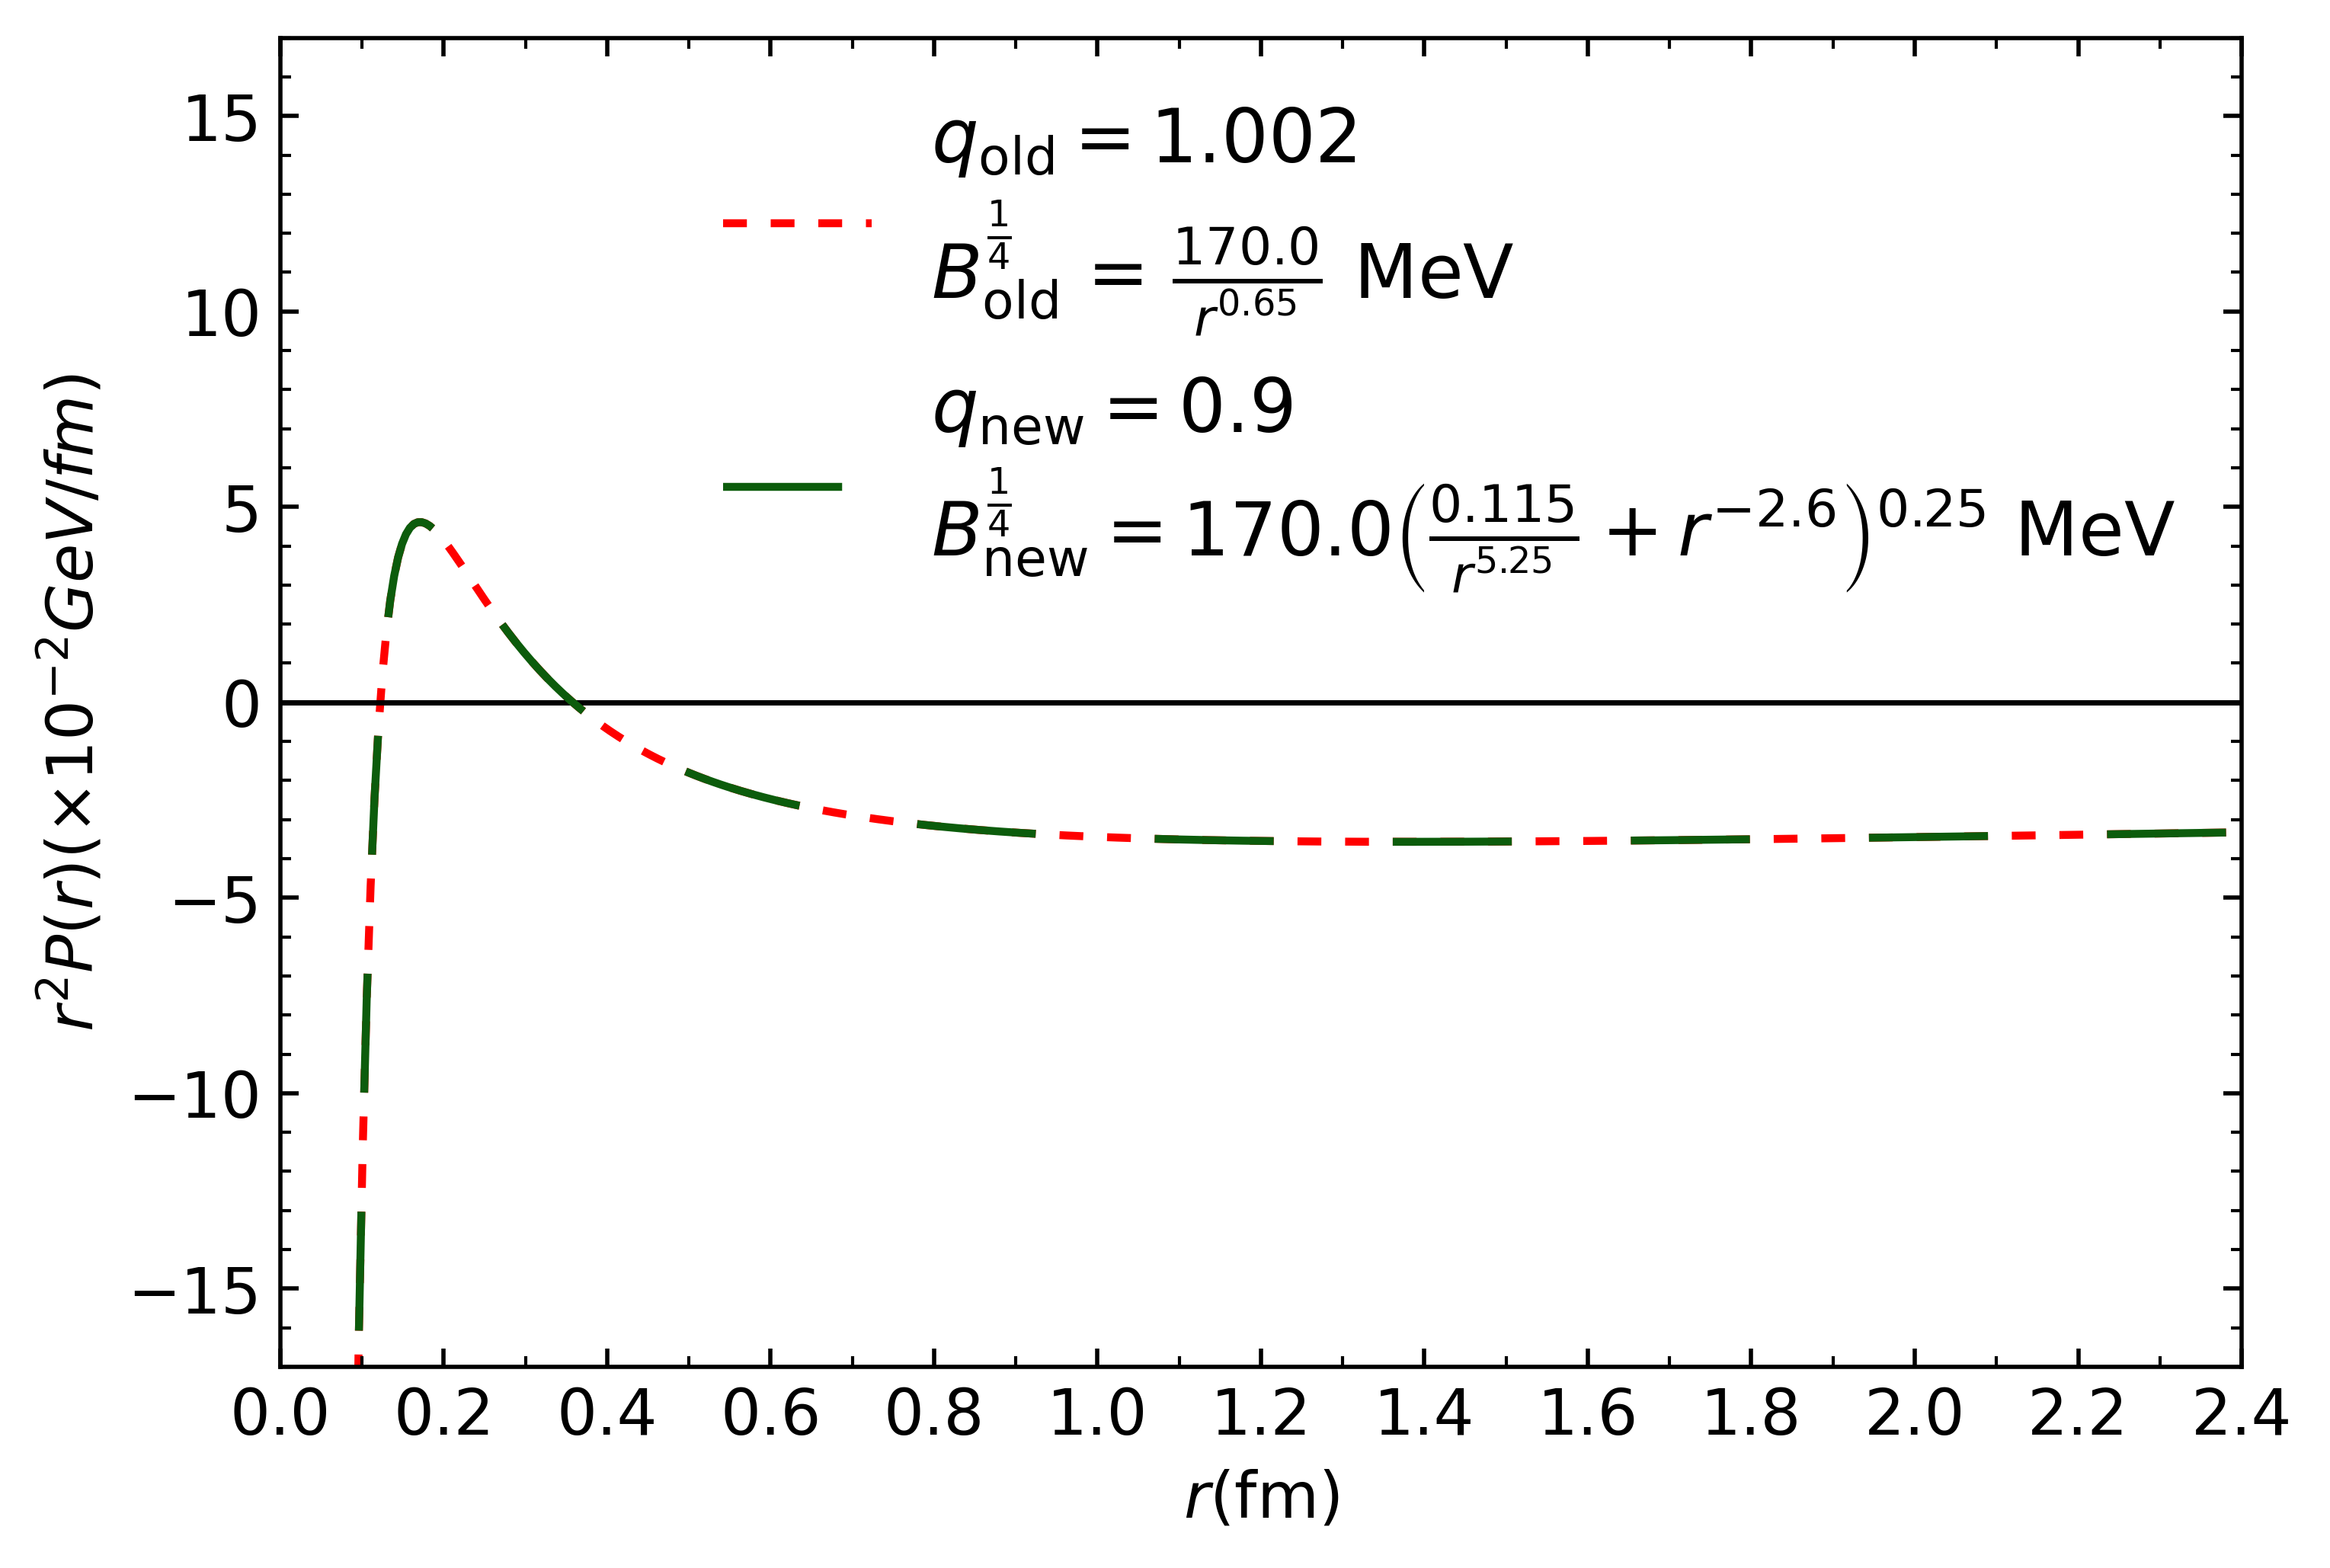
\includegraphics[width=0.75\textwidth]{./Images/Comparacion_B_old_new_combined.png}
    \caption[Comparación de perfiles con distintos \( q \)]{\emph{Comparación entre distribuciones \( r^2 P(r) \) obtenidas con \( q = 1.002 \) y una forma tradicional de \( B(r) \), y con \( q = 0.9 \) usando una forma funcional reconstruida. Ambos perfiles son compatibles en forma general, lo que respalda la hipótesis de que \( q \) puede absorber el efecto de confinamiento.}}
    \label{fig:B_reconstructed_combined}
\end{figure}

Este resultado fortalece la idea de que \( q \) puede interpretarse como un parámetro dinámico que encapsula la física del confinamiento, y no solo como un modificador estadístico.

\section{Conclusiones generales}

\begin{itemize}
    \item Se construyó un modelo efectivo basado en la estadística de Tsallis acoplado al modelo de bolsa MIT, capaz de reproducir distribuciones de presión hadrónica consistentes con QCD en el retículo.
    \item La dependencia radial del parámetro \( q(r) \) permite reinterpretar el confinamiento como un fenómeno emergente asociado a correlaciones no extensivas, prescindiendo potencialmente de la presión de bolsa fija.
    \item La validez del modelo se verificó frente a resultados de Lattice QCD y mediante reconstrucción inversa de perfiles de presión.
    \item La sensibilidad del modelo al potencial químico sugiere posibles aplicaciones en materia densa o escenarios de transición de fase (neutron stars, heavy-ion collisions, etc.).
\end{itemize}

\begin{remark}[Perspectivas]
    Futuras investigaciones podrían integrar una evolución dinámica de \( q(r,t) \), explorar efectos de anisotropías, o conectar con observables experimentales más allá de GFFs.
\end{remark}

\section*{Palabras finales}

Este trabajo presentó una formulación extendida del modelo de bolsa para nucleones mediante el uso de estadística no extensiva de Tsallis, integrando de manera natural los efectos del confinamiento y la correlación de largo alcance. Más allá de los resultados numéricos y validaciones presentadas, este estudio busca abrir nuevas líneas de exploración en la descripción efectiva de la materia hadrónica. 

Queda como perspectiva futura el desarrollo de modelos dinámicos basados en \( q(r,t) \), así como su contraste directo con datos experimentales provenientes de dispersión profunda y colisiones de alta energía.

\vspace{1em}
\noindent
\textit{“En la frontera entre estadística y confinamiento, emergen nuevas formas de comprender la estructura de la materia.”}
%\chapter{NOTAS}

\section{Notas de DeGrand sobre masas y otros parámetros de hadrones ligeros}

Los efectos de la energía cinética de quarks, energía de bolsa, masa de quarks extraño, intercambio de gluones colorados en más bajo orden, y energía asociada con ciertas fluctuaciones son incluidas. Estos son parametrizados por cuatro constantes que tienen significado fundamental y no cambian a partir de multipletes a multipletes. El ajuste al espectro es bueno. El orden de todos los estados es dado correctamente

En la teoría de quarks de estructura de hadrones tenemos las siguientes ideas fundamentales:

\begin{enumerate}
\item Los hadrones están compuestos de quarks
\item Los quarks vienen en varios ``sabores'', los tres de Gell-Mann y Zweig, aumentado quizá por nuevos quarks para nuevos grados hadrónicos de libertad como encanto, y en tres colores.
\item Los quarks interactúan entre ellos relativamente debilmente por el intercambio de un octeto de gluones acoplados sin masa, con color en la manera de Yang-Mills para sus índices de colores. 
\item La interacción debe ser débil a cortas distancias para explicar la escala en experimentos de dispersión de leptones; debe ser débil cerca de la transferencia de momento cero para contar para la falta de grandes renormalizaciones de estimaciones ingenuas del modelo de quarks de transmisiones entre bariones ligeros. 
\item La simetría SU(3) generada por la permutación de índices de color es inquebrantada. 
\item Quarks de diferentes sabores podrían tener masas diferentes para tomar en cuenta para el desglose del observador del SU(3) de Gell-Mann y para las altas masas de estados compuestas de quarks encantados.
\item Finalmente, y esencialmente, los quarks colorados y gluones colorados no son ellos mismos parte del espectro físico. Para cumplir esto, asumimos que los campos fenomenólogicos que describen la dinámica de quarks y gluones no permean todo el espació, sino prefieren estar confinados en el interior de hadrones.
\end{enumerate}

La única manera que conocemos para proporcionar la ``baja excitación'' de materia hadrónica consistente con invariancia de Lorentz es introduciendo un nuevo término, $-{g}_{\mu \nu} {\theta}_{s} B$, en el tensor de energía momento de la teoría. ${\theta}_{s}$ es una función que es unidad donde los campos de quark y gluones están definidos, cero donde no lo están. ${B}$ es una constante universal con las dimensiones de presión. Es entonces una consecuencia exacta de la simetría de color inquebrantada SU(3) que todos los estados tienen números cuánticos convencionales. Es tentador especular sobre un origen para este término poco convencional de algún lugar es más convencional parte de la teoría.



\section{Notas sobre \emph{Baryon structure in the bag theory}}

Un modelo de hadrón es considerado en que una partícula interactuando fuertemente consiste de campos confinados a una región finita de espacio que llamamos ``bolsa''. El confinamiento es logrado en una forma invariante de Lorentz suponiendo que la bolsa posee una energía positiva constante por unidad de volumen, $B$.

Para empezar, el efecto de la densidad de energía $B$ es agregar un término al tensor de energía usual:

\begin{equation}
{T}^{\mu \nu} = {T}_{\mathrm{campos}}^{\mu \nu} - {g}^{\mu \nu} B
\end{equation}

dentro de la bolsa. Fuera de la bolsa ${T}_{\mu \nu}$ se desvanece. Requerir conservación de energía momento lleva a condiciones de frontera sobre los campos en la superficie de la bolsa. Aquí especificamos los campos confinados sean sin masa, campos de espín $\frac{1}{2}$ llevando números cuánticos de quarks con color e interactuando con gluones vectoriales con color sin masa. Una consecuencia exacta de las condiciones de frontera de bolsa para tal interacción es que sólo estados singletes de color (que tienen trialidad cero) pueden existir. La constante de acoplamiento no necesita ser grande para lograr esto. Incluso cuando los campos de quarks son libres dentro de la bolsa, las ecuaciones de campo más las condiciones de frontera no son resolubles exactamente en tres dimensiones espaciales. En vez de eso las resolvemos en lo que parece ser una aproximación razonable a orden cero que es análoga a la ``teoría de Bohr'' para el átomo de hidrógeno: Las ecuaciones clásicas de movimiento admiten una clase de soluciones en que la superficie de la bolsa (en su marco de referencia) es una esfera de radio fijo. Las condiciones de frontera requieren que cada quark ocupe un modo con momento angular total $\frac{1}{2}$. Tratamos estos modos en una cavidad esférica fija como análoga a las órbitas circulares con radio fijo en la vieja teoría cuántica. El radio es entonces cuantizado por la condición que el operador número quark toma valores enteros. Para estos estados, la energía depende en qué modos están ocupados pero no en la forma del momento angular o isoespines de los quarks individuales son agregados para obtener el momento angular total e isoespín del hadrón. Así, por ejemplo, el estado de más baja energía $N(\frac{1}{2} +)$ y $\Delta(\frac{3}{2} +)$ son degenerados. Ya que $B$ es el único parámetro libre somos capaces de hacer predicciones para cantidades dimensionales tales como el momento magnético del protón y radio de carga y los splittings de masa de orden cero en el espectro bariónico. 

\subsection{Cálculos}

Las ecuaciones de movimiento y condiciones de frontera para un campo confinado de espín $\frac{1}{2}$ y sin masa

\begin{equation}
\slashed{\partial} {\psi}_{\alpha}(x) = 0
\end{equation}
 
dentro de la bolsa y

\begin{eqnarray}
i \slashed{n} {\psi}_{\alpha} (x) = {\psi}_{\alpha} (x), \\
\sum_{\alpha} n \cdot {\partial} \bar{\psi}_{\alpha} (x) {\psi}_{\alpha} (x) = 2B
\end{eqnarray}

sobre la superficie de la bolsa. ${n}_{\mu}$ es la 4-normal interior covariante a la superficie de la bolsa. $\alpha$ es un índice de simetría interna que escogemos para designar isoespín y color. Buscamos soluciones para que la frontera sea una esfera estática de radio ${R}_{0}$ en cuyo caso ${n}_{\mu} = (0, - \hat{r})$ y ecuaciones (2) se vuelven

\begin{eqnarray}
-i \hat{r} \cdot \va{\gamma}{\psi}_{\alpha} (x) = {\psi}_{\alpha}(x), \\
-\sum_{\alpha} \frac{\partial}{\partial r} \bar{\psi}_{\alpha}(x) {\psi}_{\alpha} (x) = 2B
\end{eqnarray}

en $r= {R}_{0}$.

La solución general a las ecuaciones (1) y (3) es una superposición (con coeficientes ${a}_{\alpha}$) de soluciones a la ecuación de Dirac libre:

\begin{equation}
{\psi}_{\alpha}(x,t) = \sum_{n \kappa j m} N ({\omega}_{n \kappa j}) {a}_{\alpha} (n \kappa j m) {\psi}_{n \kappa k m} (x, t).
\end{equation}

$j$ y $m$ etiquetan el modo del momento angular y su zomponente $z$. $\kappa$ es el número cuántico de Dirac\footnote{•}, $\kappa = \pm (j + \frac{1}{2})$, que diferencia los dos estados de paridad opuesta para cada valor de $j$.  El índice $n$ etiqueta frecuencias que están a ser determinadas por las condiciones de frontera lineales. La  condición de fontera cuadrática (3b) restringe los modos que pueden ser excitados. Entre otras cosas, 3b permite sólo soluciones para la ecuación de Dirac.
Para $j = \frac{1}{2}$, ya sea $\kappa = - 1$,

\begin{equation}
{\psi}_{n \, -1 \, \frac{1}{2} \, m} (x,t) = \frac{1}{\sqrt{4 \pi}} 
\left( 
\begin{array}{c}
i {j}_{0} ({\omega}_{n, \, -1} r / {R}_{0}) {U}_{m} \\
- {j}_{1} ({\omega}_{n, \, -1} r / {R}_{0}) \sigma \cdot \hat{r}{U}_{m} 
\end{array}
\right) \times {e}^{- i {\omega}_{n, \, -1} t / {R}_{0}}
\end{equation}

o ${\kappa} = 1$

\begin{equation}
{\psi}_{n \, 1 \, \frac{1}{2} \, m} (x,t) = \frac{1}{\sqrt{4 \pi}} 
\left( 
\begin{array}{c}
i{j}_{1} ({\omega}_{n, \, 1} r / {R}_{0}) \sigma \cdot \hat{r} {U}_{m} \\
{j}_{0} ({\omega}_{n, \, 1} r / {R}_{0}) {U}_{m} 
\end{array}
\right) \times {e}^{- i {\omega}_{n, \, 1} t / {R}_{0}}
\end{equation}

${U}_{m}$ es un espinos de Pauli bidimensional y ${j}_{\ell}(z)$ son las funciones de Bessel esféricas. Hemos omitido los índices $j$ sobre ${\omega}_{n \kappa}$ ya que solo $j = \frac{1}{2}$ es de interés en el presente. $N({\omega}_{n \kappa})$ es una constante de normalización escogida para conveniencia futura:

\begin{equation}
N({\omega}_{n \kappa}) \equiv \left( \frac{{\omega}_{n \kappa}^{\phantom{n \kappa} 3}}{2 {R}_{0}^{\phantom{0} 3} ({\omega}_{n \kappa} + \kappa) \sin^{2} {\omega}_{n \kappa}} \right)^{1/2}
\end{equation}

La condición de frontera lineal (3a) genera una condición eigenvalor para los modos de frecuencias ${\omega}_{n \kappa}$

$$
{j}_{0}({\omega}_{n \kappa}) = - \kappa {j}_{1} ({\omega}_{n \kappa}),
$$

o 

\begin{equation}\label{condeigenval}
\tan {\omega}_{n \kappa} = \frac{{\omega}_{n \kappa}}{{\omega}_{n \kappa} + \kappa}
\end{equation}

[Por convención escogemos $n$ positiva (negativa) secuencialmente para etiquetar las raíces positivas (negativas) de la eq 7] Las primeras soluciones a \eqref{condeigenval} son 

\begin{equation}
\begin{array}{ccc}
\kappa = - 1: & {\omega}_{1 \, -1} = 2.04; & {\omega}_{2 \, -1} = 5.40 \\
\kappa = + 1: & {\omega}_{1 \, 1} = 3.81; & {\omega}_{2 \, 1} = 7.00.
\end{array}
\end{equation}

La condición de frontera cuadrática requiere que $\sum_{\alpha} (\partial / \partial r) \bar{\psi}_{\alpha} (x) {\psi}_{\alpha}(x)$ sea independiente de tiempo y dirección para $r={R}_{0}$. La independencia angular requiere que $j = \frac{1}{2}$. Para obtener independencia temporal, ajustamos

\begin{equation}
\sum_{\alpha} {a}_{\alpha}^{*} (n \, \kappa \, j= \frac{1}{2} \, m) {a}_{\alpha} (n' \, \kappa' \, j= \frac{1}{2} \, m') = 0,
\end{equation}

a menos que $n = n'$, $\kappa = \kappa'$ o $n = -n'$, $\kappa = -\kappa'$ en cuyos casos no hay restricción ya que los términos dependientes del tiempo se cancela. La ecuación anterior es una restricción severa sobre los modos que deben ser ocupados. Deberíamos implementar la ecuación anterior requiriendo que para cada grado de libertad interno $\alpha$ sólo un modo normal, ${a}_{\alpha}(n \, \kappa \, j = \frac{1}{2} \, m)$ es excitado. Esto automáticamente será el caso para bariones de tres quarks si son requeridos a ser singletes de color.

Una vez que (9) es satisfecho, los términos independientes del tiempo en (3b) pueden ser coleccionados,

\begin{equation}
\sum_{\alpha \, n \, \kappa \, m} {\omega}_{n \kappa} {a}_{\alpha}^{*}(n \, \kappa \, \frac{1}{2} \, m) {a}_{\alpha}(n \, \kappa \, \frac{1}{2} \, m) = 4 \pi B {R}_{0}^{4},
\end{equation}


\subsubsection*{Conclusiones}

\begin{enumerate}

\item El campo en la bolsa se comporta sobre el promedio como un gas relativista perfecto; que es, la traza del tensor energía momento asociado con el campo, cuando es promediado sobre tiempo y espacio, es cero:
\begin{equation}
\left\langle \int_{R} {\mathrm{d}}^{3} x ({\Theta}_{\mu}^{\mu})_{\mathrm{campo}} \right\rangle = 0
\end{equation}
\item El volumen promediado en el tiempo de una bolsa es proporcional a su energía:
\begin{equation}
E = 4B \langle V \rangle
\end{equation}
\item El estado base y estados excitados más bajos de la bolsa contienen pocos partones de momento promedio de orden ${B}^{1/4}$ encerrados en un volumen de orden ${B}^{-3/4}$. [$B$ tiene la dimensión $(\mathrm{longitud})^{-4}$ con $\hbar=c=1$]
\item En el límite termodinámico la bolsa tiene una temperatura fija, ${T}_{0}$, independiente de su energía. ${T}_{0}$ es de orden ${B}^{-1/4}$. Esto es equivalente a las siguientes declaraciones
\begin{itemize}
\item La energía cinética promedio de los partones es de orden ${T}_{0}$ independiente de la energía de bolsa $E$ proporcionado el último es más grande que ${T}_{0}$: ${E} \gg {T}_{0}$.
\item La densidad de nivel asintótico ${\zeta(E)}$ del sistema es una función exponencial de $E$:
\[
\zeta \sim {e}^{E/{T}_{0}}
\]
\item El número, $N$, de partones más antipartones presente en el hadrón es proporcional a su energía:
\[
N \propto E/{T}_{0}
\]
\end{itemize}
\item Si la dinámica clásica es tal que hay un máximo momento angular del hadrón en una energía total dada $E$, ese máximo debe ser 
\[
{J}_{\mathrm{m\acute{a}x}} = \kappa {B}^{-1/3} {E}^{4 / 3},
\]
donde ${\kappa}$ es una constante adimensional determinada por la dinámica detallada. Si el límite clásico $({\hbar} \rightarrow 0)$ existe, las correcciones cuánticas a esta fórmula se reducirían por potencias de $E$. Si no hay trayectoria clásica a seguir, un argumento plausible sugiere que la trayectoría guía podría ser (para un gran $E$)
\[
{J}_{\mathrm{m\acute{a}x}} = {\kappa}' {B}^{-1/2} {E}^{2} \quad ({\hbar = 1}).
\]
\item El momento angular más probable para una $E$ grande está dada por 
\[
\bar{J} \propto ({B}^{-1/4} E)^{5/6}
\]
\end{enumerate}





































%\chapter{Notas sobre New Extended Model Of Hadrons de A. Chodos}

\section{Campos escalares}

Aquí empiezan con el estudio cuantitativo de las propiedades de teorías de campos confinados a una bolsa con el caso de un campo escalar único.

\subsection{Formulación del problema clásico}

Empezamos con el Lagrangiano

\begin{equation}
\begin{array}{rl}
L&= \int_{R} {\mathrm{d}}^{n-1} x (- \frac{1}{2} {\partial}_{\mu} {\phi} {\partial}^{\mu} {\phi} - B) \\
& \equiv \int_{R} {\mathrm{d}}^{n - 1} x \mathscr{L}
\end{array}
\end{equation}

(nuestra métrica es $- {g}^{00} = {g}^{ii} = 1$), donde $B$ es la constante de bolsa, que es, la densidad de energía asociada con el volumen $R$ al que los campos están confinados. La frontera de la región $R$ barre una superficie $S$ en espacio-tiempo. Las coordenadas ${X}^{\mu}$ de $S$ etiquetadas por $n-1$ parámetros ${\alpha}_{j}$,

\begin{equation}
{X}^{\mu} = {X}^{\mu}(\{ \alpha \})
\end{equation}

El vector unitario normal (${n}_{\mu}$) a esta superficie es definida para ser el vector unitario ortogonal a los $n-1$ vectores tangentes ${T}_{j}^{\mu}$:

\begin{equation}
{T}_{j}^{\mu} \equiv \frac{d}{d{\alpha}_{j}} {X}^{\mu} (\{ \alpha\}).
\end{equation}

Es útil expresar ${n}_{\mu}$ en términos de la normal (${m}_{\mu}$) a la superficie a tiempo constante ($t \equiv {x}^{0}$). Para hacer esto escogemos el parámetro ${\alpha}_{0} = t $ y reescribimos las ecuaciones anteriores como

\begin{equation}
\begin{array}{rl}
{X}^{\mu}  &= (t, X(\{ \alpha \})), \quad i = 1, \dots, n-1 \\
{T}_{j}^{\mu} & =\left\{
\begin{array}{c}
(1,\dot{X}^{i}(\{\alpha, t\})), \quad j=0\\
\left(0, \dfrac{d}{d{\alpha}_{j}} {X}^{i} (\{ \alpha \}, t)\right), \quad j =1,\dots,n-2
\end{array}
\right.
\end{array}
\end{equation}

${m}_{\mu}$ es entonces vector unitario puramente espacial [${m}_{\mu} = (0, {m}_{i})$] ortogonal a los $n - 2$ vectores tangentes ${T}_{j}^{\mu}$ ($j = 1, \dots, n - 2$):

\[
{m}_{\mu} {T}_{j}^{\mu} = 0, \quad j =1, \dots, n - 2
\]

\[
{m}_{\mu} {m}^{\mu} = 1
\]

Entonces definir

\begin{equation}
{n}_{\mu} = \frac{-({m}_{\lambda} \dot{X}^{\lambda}) {\eta}_{\mu} + {m}_{\mu}}{[1 - ({m}_{\lambda} \dot{X}^{\lambda})^{2}]^{1/2}},
\end{equation}

donde ${\eta}_{\mu}$ es el vector tipo tiempo unitario:

\[
{\eta}_{\mu} \equiv (1, 0, \dots, 0)
\]

y $\dot{X}^{\lambda} \equiv {T}_{0}^{\lambda}$. Es fácil verificar que ${n}_{\mu} {T}_{j}^{\mu} = 0$ y ${n}_{\mu}{n}^{\mu}$. Para establecer una convención escogemos que ${m}_{\mu}$ sea normal interior a la superficie espacial.

Con esta geometría preliminar en mente derivamos las ecuaciones de movimiento del sistema requiriendo que la acción $W \equiv \int_{{t}_{0}}^{{t}_{1}} dt \, L$ sea estacionario bajo variaciones del campo $\phi$ y de la frontera $S$ que se desvanece en ${t}_{0}$ y ${t}_{1}$. Estabilidad bajo variación en la frontera requiere que la densidad de Lagrange se desvanezca sobre $S$:

\begin{equation}
{\partial}_{\mu} {\phi} {\partial}^{\mu} {\phi} = - 2B \quad \mathrm{sobre} \quad S
\end{equation}

La variación de los campos generan la ecuación de Klein-Gordon dentro de la bolsa:

\begin{equation}
{\partial}_{\mu} {\partial}^{\mu} {\phi} = 0 \quad \mathrm{en} \, R
\end{equation}

y otra condición de frontera:

\begin{equation}
{n}_{\mu} {\partial}^{\mu} {\phi} = 0 \quad \mathrm{sobre} \, S
\end{equation}

Esta condición de frontera surge a partir de términos superficiales en las integraciones parciales que son realizadas para liberar la variación $\delta \phi$ de la derivada ${\partial}_{\mu}$

\subsection{Invariancia de Poincaré del problema clásico}

Las ecuaciones de movimiento son manifestamente invariante de Poincaré. Correspondiendo a esta invariancia tenemos un arreglo de momentos ${P}_{\mu}$ y generadores de rotación de Lorentz ${M}_{\mu \nu}$ que deberían ser independientes del tiempo. Estos pueden ser construidos por medio del teorema de Noether a partir del Lagrangiano. 

Las corrientes conservadas localmente son idénticas a esas del campo de Klein Gordon libre excepto por términos involucrando la densidad de energía $B$:

\begin{equation}
{T}_{\mu \nu} \equiv {g}_{\mu \nu} \mathscr{L} + {\partial}_{\mu} {\phi} {\partial}_{\nu} {\phi},
\end{equation}

\begin{equation}
{M}_{\mu \nu \lambda} = {x}_{\mu} {T}_{\nu \lambda} - {x}_{\nu} {T}_{\mu \lambda}
\end{equation}

con

\[
{\partial}^{\nu} {T}_{\mu \nu} = {\partial}^{\lambda} {M}_{\mu \nu \lambda} = 0
\]

Para mostrar la constancia de las cargas correspondientes considerar la integral de la divergencia de una corriente conservada sobre el "hipertubo mundial" de la bolsa:

\begin{equation}
0 = \int_{V} {d}^{n} x \, {\partial}_{\mu} \mathscr{J}^{\mu} \quad (\mathrm{donde} {\partial}_{\mu} \mathscr{J}^{\mu} = 0)
\end{equation}

$V$ es el volumen espacio temporal recorrido por la bolsa y está ligado por dos hipersuperficies de tipo espacial y luz ${R}_{1}$ y ${R}_{2}$ que pueden ser tomadas como superficies de tiempo constante.

Integrando la ecuación anterior obtenemos

\begin{equation}
Q \equiv \int_{{R}_{1}} ds \, {n}_{\mu} \mathscr{J}^{\mu} = \int_{{R}_{2}} ds \, {n}_{\mu} \mathscr{J}^{\mu} - \int_{S} ds \, {n}_{\mu} \mathscr{J}^{\mu}
\end{equation}

donde $ds$ es el elemento de superficie sobre las superficies $(n-1)$ dimensionales ${R}_{1}$, ${R}_{2}$, y $S$. Para las corrientes conservadas de (3.9) y (3.10) es fácilmente mostrado que ${n}_{\mu} \mathscr{J}^{\mu } = 0$ sobre $S$ con el auxilio de la condición de frontera (3.8). Por lo tanto hay independencia temporal de las cargas convencionales. Para completez, anotamos las expresiones para ${P}_{\mu}$ y ${M}_{\mu \nu}$ definidas sobre superficies de tiempo constante:

\begin{equation}
{P}_{\mu} \equiv \int_{R} {d}^{n-1} x {T}_{\mu}^{\phantom{\mu} 0}
\end{equation}

\begin{equation}
{M}_{\mu \nu} \equiv \int_{R} {d}^{n-1} x \, ({x}_{\mu} {T}_{\nu}^{0} - {x}_{\nu} {T}_{\mu}^{0}).
\end{equation}

Ya que la función primaria de las condiciones de frontera es garantizar la conservación de los generadores de Poincaré, podemos preguntar si existe un conjunto alternativo de condiciones de frontera, aparte de (3.6) y 3.9, que lograran esta meta.


\subsection{Mecánica clásica en dos dimensiones}

En una dimensión espacial y una temporal, las ecuaciones de movimiento del campo escalar confinado a una bolsa se simplifican considerablemente.

Ya que el campo dentro de la bolsa es sin masa, es conveniente trabajar con variables de cono de luz:

\[
{x}^{+} \equiv \tau \equiv \frac{1}{\sqrt{2}}(t + z),
\]

\[
{x}^{-} \equiv x \equiv \frac{1}{\sqrt{2}} (t -z)
\]

Usando variables de cono de luz, el tensor métrico es fuera de la diagonal ${g}^{+-} = {g}^{-+} = -1$, ${g}^{++} ={g}^{--} = 0$. Denotamos las derivadas con respecto a $\tau$ por puntos:

\[
{\partial}_{+} {\phi} (x, \tau) = \frac{\partial}{\partial \tau} {\phi} (x, \tau) = \dot{\phi} (x,\tau)
\]

y derivadas con respecto a $x$ por primas:

\[
{\partial}_{-} {\phi} (x, \tau) = \frac{\partial}{\partial x} \phi (x, \tau) = {\phi}' (x, \tau).
\]

\subsubsection{Solución al problema clásico}

En dos dimensiones y en coordenadas de cono de luz, la ecuación de movimiento y las condiciones de frontera se reducen a

\begin{equation}
\frac{{\partial}^{2}}{\partial x \partial \tau} {\phi} (x, \tau) = 0, \; \mathrm{en} \; R
\end{equation}

\begin{equation}
\dot{\phi} ({x}_{i} (\tau), \tau) {\phi}' ({x}_{i}(\tau), \tau) = - B, \quad i =0,1
\end{equation}

\begin{equation}
{\phi}({x}_{i}(\tau), \tau) = 0,
\end{equation}

donde ${x}_{i} (\tau)$ ($i = 0, 1$) son los dos puntos que encierran la bolsa. 

Para resolver la ecuación de onda, podemos proponer una solución de la forma

\begin{equation}
{\phi}(x, \tau) = {f}(\tau) + g(x).
\end{equation}

Las condiciones de frontera pueden ser reescritas en términos de ${f}(\tau)$ y ${g}(x)$:

\begin{equation}
\dot{f} (\tau) {g}' ({x}_{i}(\tau)) = - B, \quad i=0, 1
\end{equation}

\begin{equation}
\dot{f}(\tau) + \dot{x}_{i} (\tau) {g}' ({x}_{i} (\tau)) = 0,
\end{equation}

donde hemos diferenciado (3.15c) para obtener (3.17b). Las constantes del movimiento están dadas por (3.13):

\begin{equation}
{P}^{-} \equiv H = B ({x}_{1} (\tau) - {x}_{0} (\tau)),
\end{equation}

\begin{equation}
{P}^{+} \equiv P = \int_{{x}_{0}(\tau)}^{{x}_{1}(\tau)} dx \, [g'(x)]^{2},
\end{equation}

\begin{equation}
{M}^{+-} \equiv M = H \tau - \int_{{x}_{0}(\tau)}^{{x}_{1}(\tau)} dx \, x [{g}' (x)]^{2}
\end{equation}

La independencia temporal de $H$, $P$, y $M$ puede ser verificada con la ayuda de las condiciones de frontera (3.17). Por ejemplo, una combinación ajustable de las ecuaciones (3.17) lleva a

\[
\dot{x}_{i}(\tau) = \frac{[\dot{f}(\tau)]^{2}}{B},
\]

tal que $\dot{x}_{i}(\tau)$ es independiente de $i$ y $\dot{H} = 0$.

Para seguir encontraremos conveniente linealizar las condiciones de frontera. Esto puede ser hecho definiendo un nuevo parámetro espacial ${\sigma} = {\sigma}(x)$ de acuerdo a la ecuación diferencial

\begin{equation}
\frac{d \sigma}{d x} = \frac{1}{p} [g'(x)]^{2}
\end{equation}

y condición inicial $\sigma ( {x}_{0}(0)) = 0$, donde $p$ es una constante que será especificada después.
Definimos un nuevo campo $\tilde{g} (\sigma)$ en términos de $g(x)$ por este cambio de variables independientes,

\begin{equation}
\tilde{g} (\sigma) \equiv {g} (x(\sigma))
\end{equation}

$x(\sigma)$ será determinado a partir del inverso de

\begin{equation}
\frac{dx}{d\sigma} = \frac{1}{p} [\tilde{g}'(\sigma)],
\end{equation}

donde $\tilde{g}' (\sigma) \equiv (\frac{d}{d\sigma}) \tilde{g} (\sigma)$. Las fronteras de la bolsa son ${\sigma}_{i} (\tau) \equiv \sigma ({x}_{i} (\tau))$. Cuando es descrito en términos de $\sigma$, el movimiento de frontera será bastante más simple. Cuando transformamos a $\sigma$ como variable independiente (3.17) se vuelve

\begin{equation}
\dot{f}(\tau) = -\frac{B}{p} \tilde{g}'({\sigma}_{i}(\tau)),
\end{equation}

\begin{equation}
\dot{f}(\tau) + \dot{\sigma}_{i} (\tau) \tilde{g}' ({\sigma}_{i} (\tau)) = 0
\end{equation}

tal que $\dot{\sigma}_{i} (\tau) = \frac{B}{p}$. Usando la condición inicial ${\sigma} ({x}_{0}(0)) = {\sigma}_{0} = 0$, ${\sigma}_{0}(\tau) = \frac{B \tau}{p}$, ${\sigma}_{1}(\tau) = (B \tau / p) + {\sigma}_{1}$, donde ${\sigma}_{1}$ es una constante de integración. Para especificar ${\sigma}_{1}$ y $p$ considerar el momento (3.18b) en conjunción con (3.19):

\[
P = p ({\sigma}_{1} (\tau) - {\sigma}_{0} (\tau)) = p {\sigma}_{1}
\]

Consecuentemente, si escogemos por conveniencia $p$ sea la constante $P$, entonces ${\sigma}_{1} = 1$ y

\begin{equation}
{\sigma}_{1} (\tau) = \frac{B \tau}{P} + 1
\end{equation}

\begin{equation}
{\sigma}_{0} (\tau) = \frac{B \tau}{P}
\end{equation}

La solución es ahora inmediato 


\section{Campos fermiónicos} 

\subsection{Declaración de las condiciones de frontera}

Supongamos que consideramos un solo campo de Dirac en la bolsa descrito por la acción

\begin{equation}
{W}_{1} = \int_{V} {d}^{4} x [\frac{1}{2} i (\bar{\psi} \overleftrightarrow{\slashed{\partial}} \psi) - ]
\end{equation}




\chapter{Notas sobre Masses and other parameters of the light hadrons DeGrand }

Las masas y parámetros estáticos de hadrones ligeros 

Los efectos  de la energía cinética de quark, energía de bolsa, masa de quark extraño, intercambio de gluon colorado a más bajo orden, y energía asociada con ciertas fluctuaciones cuánticas son incluidas. Estas son parametrizadas por cuatro constantes que tienen significancia fundamental y no cambiar de multiplete a multiplete. El ajuste al espectro es bueno.

Momentos magnético, constantes de decaimiento débil, y el radio de carga son calculados. Donde comparación con experimento es posible.

\section{Introducción}

Durante la decada pasada, una teoría de quarks de estructura de hadron ha sido desarrollada que es exitosa en interpretar vastas cantidades de datos experimentales de unas pocas ideas simples extraordinariamente. Los ingredientes de esta teoría son como sigue:

\begin{enumerate}
\item Hadrones están compuestos de quarks. Los quarks vienen en varios "sabores", los tres de Gell - Mann y Zweig, aumentado quizá por nuevos quarks para nuevos grados de libertad hadrónicos tales como encanto, y 3 colores.
\item Los quarks interactuan entre ellos mismos relativamente débilmente por el intercambio de un octeto de gluones acoplados colorados, sin masa en la manera de Yang Mills a sus índices de colores. 
\item La interacción debe ser débil a cortas distancias para explicar escala en experimentos de dispersión de leptones; debe ser débil cerca de la transferencia de momento cero para tomar en cuenta para la falta de grandes renormalizaciones de modelo de quark sencillo estima de transiciones entre bariones ligeros.
\item La simetría SU(3) generada por la permutación de índices de color es inquebrantable.
\item Los quarks de diferentes sabores pueden tener diferentes masas para dar cuenta del desglose observado del SU(3) de Gell Mann y para las altas masas de estados compuestos de quarks encantados si eso es lo que son $J(3100)$ y $\psi(3700)$
\end{enumerate}

Finalmente, y esencialmente, quarks colorados y gluones colorados no son ellos mismos parte del espectro físico.

Los grados de libertad de quark-gluon pueden similarmente caracterizar variables colectivas describiendo la "baja excitación" de materia hadrónica. La única manera que sabemos de proporcionar una descripción de esto consistente con invariancia de lorentz es introduciendo un nuevo término, $-{g}_{\mu \nu} {\theta}_{s} B$, en el tensor de energía momento de la teoría \cite{DeTar_1983, Chodos_1974, Han_1965, Greiner2001, DeGrand_1975}.

\[
{\gamma}^{0} = \left(
\begin{array}{cc}
{I}_{2} & 0\\
0 & -{I}_{2}
\end{array}
\right)
\]




% ================================================================================================================================
% Apéndices
% ================================================================================================================================
\appendix
\renewcommand{\appendixname}{Apéndice}
\chapter{Derivaciones Matemáticas Detalladas}\label{app:math_derivations}

% =====================Estilo de página================================
\pagestyle{fancy}
\fancyhf{} % Limpia todos los campos de encabezado y pie de página
% \fancyhead[LE]{\nouppercase{\textit{\rightmark}}} % Sección en páginas pares (izquierda)
% \fancyhead[RO]{\nouppercase{\textit{\rightmark}}} % Sección en páginas impares (derecha)
\fancyhead[RE]{\nouppercase{\hfill \textbf{\leftmark}}} % Capítulo en páginas impares (izquierda)
\fancyhead[LO]{\nouppercase{\textbf{\leftmark} \hfill}} % Capítulo en páginas pares (derecha)
\fancyfoot[LE]{\nouppercase{\thepage \hfill {Pressure Distribution Inside Nucleons in a Tsallis-MIT Bag Model}}} % Pie de página en páginas pares
\fancyfoot[RO]{\nouppercase{{Pressure Distribution Inside Nucleons in a Tsallis-MIT Bag Model} \hfill \thepage}} % Pie de página en páginas impares
% =====================================================================

%%%%%%%%%%%%%%%%%%%%%%%%%%%%%%%%%%%%%%%%%%%%%%%%%%%%%%%%%%%%%%%%%%%%%%%%%%%%%%%%%%%%%%%%%%%%%%%%%%%%%%%%%%%%%

\section{Derivaciones detalladas del gas de gluones}
\label{app:BE_derivation}

En esta sección se derivan de forma detallada las expresiones termodinámicas del gas de gluones modelado como un sistema ideal de Bose-Einstein ultrarrelativista. Estas expresiones se utilizan en la sección \ref{sec-PresTsa} para el desarrollo de la entropía y presión dentro del hadrón bajo estadística de Tsallis.

% ------------------------------------------------------------------------------------------------ %

\subsection{Densidad de estados y función de partición}

Para gluones (bosones sin masa), la relación energía-momento en el régimen ultrarrelativista está dada por:

\begin{equation}
\epsilon = p c = \hbar c |\vec{k}|,
\end{equation}

donde \( |\vec{k}| \) es el módulo del vector de onda y \( p \) la magnitud del momento lineal. 

La densidad de estados en el espacio de fases tridimensional, considerando volumen \( V \), es:

\begin{equation}
g(\epsilon)\,d\epsilon = g_G \frac{V \epsilon^2 d\epsilon}{\pi^2 (hc)^3},
\end{equation}

donde \( g_G = 16 \) es el factor de degeneración para gluones (8 tipos de gluones × 2 polarizaciones transversales). Esta expresión surge de contar los modos disponibles en una caja cúbica de volumen \( V \) con condiciones de frontera periódicas, y se utiliza para convertir sumas discretas en integrales continuas.

La función de partición del sistema se expresa como:

\begin{equation}
\Xi = \prod_j \frac{1}{1 - e^{-\beta \epsilon_j}},
\end{equation}

donde \( j \) es un índice que recorre todos los niveles de energía disponibles y \( \beta = ({k}_{\mathrm{B}} T)^{-1} \).

% ------------------------------------------------------------------------------------------------ %

\subsection{Integrales fundamentales}

Las cantidades termodinámicas se expresan en términos de integrales de la forma:

\begin{equation}
I_n = \int_0^\infty \frac{\epsilon^n d\epsilon}{e^{\beta\epsilon} - 1},
\end{equation}

las cuales se evalúan fácilmente mediante el cambio de variable \( x = \beta \epsilon \), resultando en:

\begin{equation}
I_n = \frac{1}{\beta^{n+1}} \int_0^\infty \frac{x^n dx}{e^x - 1} = \frac{\Gamma(n+1)\zeta(n+1)}{({k}_{\mathrm{B}} T)^{n+1}},
\end{equation}

donde \( \Gamma \) es la función gamma y \( \zeta \) es la función zeta de Riemann.

Los valores específicos de estas integrales más relevantes son:

\begin{align}
\int_0^\infty \frac{x^2 dx}{e^x - 1} &= 2\zeta(3) \approx 2.404, \\
\int_0^\infty \frac{x^3 dx}{e^x - 1} &= \frac{\pi^4}{15} \approx 6.494.
\end{align}

% ------------------------------------------------------------------------------------------------ %

\subsection{Energía del sistema}
\label{app:BE-Energy}

La energía total del sistema se obtiene integrando sobre todos los modos disponibles, ponderados por su ocupación térmica:

\begin{equation}
E_G = \int_0^\infty g(\epsilon) \, \epsilon \, f_{\mathrm{BE}}(\epsilon)\, d\epsilon,
\end{equation}

donde \( f_{\mathrm{BE}}(\epsilon) = \frac{1}{e^{\beta\epsilon} - 1} \) es la distribución de ocupación de Bose-Einstein. Sustituyendo y usando el resultado anterior para la integral:

\begin{equation}
E_G = \frac{g_G V}{\pi^2 (hc)^3} \int_0^\infty \frac{\epsilon^3 d\epsilon}{e^{\beta\epsilon} - 1} = \frac{g_G V}{\pi^2 (hc)^3} \frac{\pi^4 ({k}_{\mathrm{B}} T)^4}{15}.
\end{equation}

En unidades naturales \( \hbar = c = {k}_{\mathrm{B}} = 1 \), se simplifica a:

\begin{equation}
E_G = g_G \frac{\pi^2}{30} V T^4.
\end{equation}

% ------------------------------------------------------------------------------------------------ %

\subsection{Presión}
\label{app:BE-Pressure}

La presión se obtiene a partir del potencial gran canónico, el cual se relaciona con la función de partición mediante:

\begin{equation}
\ln \Xi = -\frac{g_G V}{\pi^2 (hc)^3} \int_0^\infty \epsilon^2 \ln(1 - e^{-\beta\epsilon}) d\epsilon.
\end{equation}

Realizando una integración por partes y usando identidades estándar de integrales, se encuentra que:

\begin{equation}
\ln \Xi = \frac{g_G V}{3\pi^2 (hc)^3 \beta} \int_0^\infty \frac{\epsilon^3 d\epsilon}{e^{\beta\epsilon} - 1}.
\end{equation}

La presión se calcula como:

\begin{equation}
P_G = \frac{{k}_{\mathrm{B}} T}{V} \ln \Xi = \frac{g_G \pi^2 ({k}_{\mathrm{B}} T)^4}{90 (hc)^3},
\end{equation}

y en unidades naturales:

\begin{equation}
P_G = \frac{1}{3} \frac{E_G}{V} = g_G \frac{\pi^2}{90} T^4.
\end{equation}

Esto refleja la relación característica entre presión y energía de un gas ultrarrelativista.

% ------------------------------------------------------------------------------------------------ %

\subsection{Entropía}
\label{app:BE-Entropy}

La entropía se puede obtener directamente a partir de la energía utilizando la identidad:

\begin{equation}
S_G = \left( \frac{\partial E_G}{\partial T} \right)_{V} = \frac{4}{3} \frac{E_G}{T}.
\end{equation}

Sustituyendo la expresión de la energía:

\begin{equation}
S_G = g_G \frac{4\pi^2}{90} V T^3.
\end{equation}

% ------------------------------------------------------------------------------------------------ %

\subsection{Justificación de \(\mu = 0\) para gluones}

En sistemas con partículas sin número conservado, como los gluones, el potencial químico se anula en equilibrio termodinámico. Esto se debe a que los gluones pueden crearse y aniquilarse libremente, de modo que no existe una restricción asociada a su número total.

\begin{equation}
N_G(T,V,0) = \frac{g_G V}{\pi^2 (hc)^3} \int_0^\infty \frac{\epsilon^2 d\epsilon}{e^{\beta\epsilon} - 1} \propto T^3,
\end{equation}

lo que confirma que la ocupación de estados sigue siendo finita sin necesidad de introducir un término de control para \( N \). Por tanto, se toma:

\begin{equation}
\mu_G = 0.
\end{equation}

% ------------------------------------------------------------------------------------------------ %

\subsubsection*{Resumen de resultados fundamentales}

\begin{itemize}
    \item Energía total: \( E_G = g_G \frac{\pi^2}{30} V T^4 \)
    \item Presión: \( P_G = \frac{1}{3} \frac{E_G}{V} = g_G \frac{\pi^2}{90} T^4 \)
    \item Entropía: \( S_G = g_G \frac{4\pi^2}{90} V T^3 \)
    \item Potencial químico: \( \mu_G = 0 \)
\end{itemize}

Estas expresiones son esenciales para extender el análisis al marco de la estadística no extensiva de Tsallis, donde las correlaciones entre grados de libertad se introducen mediante el parámetro \( q \).


%%%%%%%%%%%%%%%%%%%%%%%%%%%%%%%%%%%%%%%%%%%%%%%%%%%%%%%%%%%%%%%%%%%%%%%%%%%%%%%%%%%%%%%%%%%%%%%%%%%%%%%%%%%%%

\section{Derivaciones detalladas del gas de quarks}
\label{app:FD_derivation}

El gas de quarks se modela como un sistema ideal de partículas fermiónicas ultrarrelativistas sin masa. Dado que se consideran quarks y antiquarks en equilibrio, el sistema incluye dos gases acoplados con potenciales químicos opuestos. Esta derivación permite obtener expresiones para la energía, presión, número neto de partículas y entropía.

% ------------------------------------------------------------------------------------------------ %

\subsection{Descripción del sistema}

Se considera un sistema compuesto por quarks y antiquarks con las siguientes características:

\begin{itemize}
    \item[$\triangleright$] Relación energía-momento: \( \epsilon = pc = \hbar c |\vec{k}| \), válida en el límite \( m \rightarrow 0 \).
    \item[$\triangleright$] Simetría partícula-antipartícula: \( \mu_{\text{quark}} = -\mu_{\text{antiquark}} = \mu \).
    \item[$\triangleright$] Factor de degeneración: \( g_Q = 12 \) (2 espines × 3 colores × 2 sabores \( u,d \)).
    \item[$\triangleright$] Estadística Fermi-Dirac:
    \[
    f_{\mathrm{FD}}^{\pm}(\epsilon) = \frac{1}{e^{\beta(\epsilon \mp \mu)} + 1}.
    \]
\end{itemize}

% ------------------------------------------------------------------------------------------------ %

\subsection{Número neto de partículas}

El número promedio total de quarks y antiquarks se obtiene sumando sobre los estados energéticos ocupados:

\begin{align}
N_+ &= \int_0^\infty g(\epsilon) f_{\mathrm{FD}}^+(\epsilon) d\epsilon, \\
N_- &= \int_0^\infty g(\epsilon) f_{\mathrm{FD}}^-(\epsilon) d\epsilon,
\end{align}

donde \( f_{\mathrm{FD}}^\pm \) son las distribuciones de quarks y antiquarks. La densidad de estados para partículas sin masa es la misma que para bosones:

\[
g(\epsilon) d\epsilon = \frac{g_Q V \epsilon^2 d\epsilon}{\pi^2 (hc)^3}.
\]

El exceso neto de quarks se define como:

\begin{equation}\label{eq-FD-Excedente-app}
N = N_+ - N_- = \frac{g_Q V}{\pi^2 (hc)^3} \int_0^\infty \epsilon^2 \left[ f_{\mathrm{FD}}^+(\epsilon) - f_{\mathrm{FD}}^-(\epsilon) \right] d\epsilon.
\end{equation}

Esta integral puede resolverse analíticamente en unidades naturales \( \hbar = c = \text{k}_{\mathrm{B}} = 1 \), resultando en:

\begin{equation}
N = \frac{g_Q V}{6} \left( \pi^2 \mu T^2 + \mu^3 \right).
\end{equation}

% ------------------------------------------------------------------------------------------------ %

\subsection{Energía total del sistema}

La energía total incluye la contribución de quarks y antiquarks:

\begin{equation}
E_Q = \int_0^\infty g(\epsilon) \, \epsilon \left[ f_{\mathrm{FD}}^+(\epsilon) + f_{\mathrm{FD}}^-(\epsilon) \right] d\epsilon.
\end{equation}

Evaluando la integral, se obtiene:

\begin{equation}
E_Q = g_Q V T^4 \left[ \frac{7\pi^2}{120} + \frac{1}{4} \left( \frac{\mu}{T} \right)^2 + \frac{1}{8\pi^2} \left( \frac{\mu}{T} \right)^4 \right].
\end{equation}

% ------------------------------------------------------------------------------------------------ %

\subsection{Presión}

En un gas ultrarrelativista sin masa, la relación fundamental entre energía y presión es:

\begin{equation}
P_Q = \frac{1}{3} \frac{E_Q}{V}.
\end{equation}

Sustituyendo la expresión para \( E_Q \):

\begin{equation}
P_Q = \frac{g_Q T^4}{3} \left[ \frac{7\pi^2}{120} + \frac{1}{4} \left( \frac{\mu}{T} \right)^2 + \frac{1}{8\pi^2} \left( \frac{\mu}{T} \right)^4 \right].
\end{equation}

% ------------------------------------------------------------------------------------------------ %

\subsection{Entropía}

La entropía se obtiene a partir de la relación:

\begin{equation}
S_Q = \frac{4}{3} \frac{E_Q}{T} - \frac{\mu N}{T}.
\end{equation}

Sustituyendo las expresiones de \( E_Q \) y \( N \), se llega a:

\begin{equation}
S_Q = g_Q V T^3 \left[ \frac{7\pi^2}{90} + \frac{1}{6} \left( \frac{\mu}{T} \right)^2 \right].
\end{equation}

% ------------------------------------------------------------------------------------------------ %

\subsubsection*{Resumen de resultados fundamentales}

\begin{itemize}
    \item \textbf{Número neto de quarks:} \( N = \dfrac{g_Q V}{6} \left( \pi^2 \mu T^2 + \mu^3 \right) \)
    \item \textbf{Energía:} \( E_Q = g_Q V T^4 \left[ \dfrac{7\pi^2}{120} + \dfrac{1}{4} \left( \dfrac{\mu}{T} \right)^2 + \dfrac{1}{8\pi^2} \left( \dfrac{\mu}{T} \right)^4 \right] \)
    \item \textbf{Presión:} \( P_Q = \dfrac{1}{3} \dfrac{E_Q}{V} \)
    \item \textbf{Entropía:} \( S_Q = g_Q V T^3 \left[ \dfrac{7\pi^2}{90} + \dfrac{1}{6} \left( \dfrac{\mu}{T} \right)^2 \right] \)
\end{itemize}

Estas expresiones son esenciales para el cálculo de la entropía total del sistema quark-gluón bajo el enfoque de Tsallis en la sección \ref{sec-PresTsa}, donde la no extensividad se introduce mediante una correlación entre las contribuciones individuales de quarks y gluones.

%%%%%%%%%%%%%%%%%%%%%%%%%%%%%%%%%%%%%%%%%%%%%%%%%%%%%%%%%%%%%%%%%%%%%%%%%%%%%%%%%%%%%%%%%%%%%%%%%%%%%%%%%%%%%

\section{Derivación de la presión en el modelo de Tsallis}
\label{app:Tsallis-pressure}

Partimos de la relación de Maxwell para sistemas termodinámicos generalizados:

\begin{equation}\label{eq:Maxwell-Tsallis-appendix}
\left. \frac{\partial S_q}{\partial V} \right|_{T,\mu} = \left. \frac{\partial P_q}{\partial T} \right|_{V,\mu},
\end{equation}

donde \( S_q \) representa la entropía total del sistema (quarks + gluones) bajo el formalismo de Tsallis. Asumimos que el volumen \( V \) y la temperatura \( T \) son cantidades extensivas, mientras que la entropía y la presión pueden presentar no extensividad a través del parámetro \( q \).

La expresión de entropía total está dada por (véase ecuación \ref{eq-Tsallis-Entropy-final}):

\begin{equation}
S_q = \left[ \frac{74\pi^2}{45} + 2\left( \frac{\mu}{T} \right)^2 \right] V T^3 + \frac{128\pi^2}{15}(1-q)\left[ \frac{7\pi^2}{90} + \frac{1}{6} \left( \frac{\mu}{T} \right)^2 \right] V^2 T^6.
\end{equation}

Al derivar con respecto a \( V \), obtenemos:

\begin{equation}\label{eq:dSdV}
\left. \frac{\partial S_q}{\partial V} \right|_{T,\mu} = \left[ \frac{74\pi^2}{45} + 2\left( \frac{\mu}{T} \right)^2 \right] T^3 + 2 \cdot \frac{128\pi^2}{15}(1-q)\left[ \frac{7\pi^2}{90} + \frac{1}{6} \left( \frac{\mu}{T} \right)^2 \right] V T^6.
\end{equation}

Aplicando la relación de Maxwell \eqref{eq:Maxwell-Tsallis-appendix}, esta derivada corresponde a la derivada de la presión con respecto a la temperatura:

\begin{equation}
\left. \frac{\partial P_q}{\partial T} \right|_{V,\mu} = \left. \frac{\partial S_q}{\partial V} \right|_{T,\mu}.
\end{equation}

Para obtener \( P_q \), integramos la expresión \eqref{eq:dSdV} con respecto a \( T \):

\begin{equation}
\begin{split}
P_q = & \left[ \frac{74\pi^2}{45} + 2\left( \frac{\mu}{T} \right)^2 \right] \int T^3 \, dT \\
& + 2 \cdot \frac{128\pi^2}{15}(1-q) \left[ \frac{7\pi^2}{90} + \frac{1}{6} \left( \frac{\mu}{T} \right)^2 \right] V \int T^6 \, dT + C(V, \mu, q).
\end{split}
\end{equation}

Al integrar término a término e imponer la condición de consistencia con el caso \( q = 1 \), se determina la constante de integración \( C(V, \mu, q) \) de modo que:

\[
P_{q=1} = P_Q + P_G.
\]

Usando las expresiones conocidas para gases de quarks (Fermi-Dirac) y gluones (Bose-Einstein) en el límite de Boltzmann-Gibbs:

\begin{equation}
P_{q=1} = \left[\frac{37\pi^2}{90} + \left(\frac{\mu}{T} \right)^2 + \frac{1}{2\pi^2} \left(\frac{\mu}{T} \right)^4 \right] T^4,
\end{equation}

lo que permite determinar explícitamente \( C(V, \mu, q) \). Finalmente, sustituimos y simplificamos para obtener la expresión completa:

\begin{equation}\label{eq:FinalTsallisPressureAppendix}
P_q = \left[ \frac{37\pi^2}{90} + \left( \frac{\mu}{T} \right)^2 + \frac{1}{2\pi^2} \left( \frac{\mu}{T} \right)^4 \right] T^4 + \frac{256\pi^2}{15}(1-q) \left[ \frac{\pi^2}{90} + \frac{1}{30} \left( \frac{\mu}{T} \right)^2 \right] V T^7.
\end{equation}

Esta expresión generaliza la presión del sistema a partir de la entropía de Tsallis e incluye explícitamente un término no extensivo que escala con \( V T^7 \). Este término se anula en el límite \( q \to 1 \), recuperando así la expresión clásica de Boltzmann-Gibbs.

\subsection*{Resumen esquemático: derivación de la energía en Tsallis} \label{app:flow}

\begin{figure}[H]
\centering
\begin{tikzpicture}[
    node distance=1.5cm,
    rect/.style={rectangle, draw, rounded corners=5pt, minimum width=3.5cm, minimum height=1cm, align=center, fill=blue!5},
    arrow/.style={->, >=stealth, thick}
]
% Nodos
\node (S) [rect] {Entropía total \\ $S_q = S_Q + S_G + (1-q)S_Q S_G$};
\node (P) [rect, below of=S] {Relación de Maxwell \\ $\displaystyle\frac{\partial S_q}{\partial V} = \frac{\partial P_q}{\partial T}$};
\node (E) [rect, below of=P] {Densidad de energía \\ $\epsilon_q = -P_q + T s_q + \mu \Delta n$};

% Flechas
\draw [arrow] (S) -- (P);
\draw [arrow] (P) -- (E);

% Anotación
\node [right=0.5cm of E, text width=4.5cm, anchor=west, font=\small] {
\begin{itemize}
\item[$\triangleright$] En este modelo, \( \Delta n = 0 \)
\item[$\Rightarrow$] \( \mu \Delta n = 0 \), ya que el número total de partículas no se ve afectado por las correlaciones.
\end{itemize}
};
\end{tikzpicture}
\caption{Flujo de derivación de la densidad de energía en el modelo de Tsallis.}
\label{fig:derivation-flow}
\end{figure}
\section{Modo fundamental y presión de bolsa en el modelo de bolsa}
\label{app:bag-pressure}

En el modelo de bolsa del MIT, las soluciones permitidas para las funciones de onda de los quarks están determinadas por una condición de contorno sobre la superficie de la bolsa esférica. Esta condición conduce a una ecuación de autovalores, cuyas soluciones discretas determinan los posibles modos normales.

\subsection{Condición de cuantización}

La ecuación de cuantización más baja para el modo esférico se escribe como:

\begin{equation}
\omega_{n\kappa} = p_{n\kappa} R,
\end{equation}

donde \( \omega_{n\kappa} \) es la energía adimensionalizada, \( p_{n\kappa} \) es el momento cuántico, y \( R \) es el radio de la bolsa. El modo fundamental (\( n = 1, \kappa = -1 \)) tiene el valor:

\begin{equation}
\omega_0 = \omega_{1, -1} \approx 2.04.
\end{equation}

Este valor define un momento máximo accesible para los quarks dentro de la bolsa:

\begin{equation}
p_{\text{max}} = \frac{\omega_0}{R}.
\end{equation}

\subsection{Energía de quarks confinados}

Bajo este límite, la energía cinética de los quarks (en ausencia de potencial químico y masa) se expresa como:

\begin{equation}
E_Q = \frac{(g_Q + g_{\bar{Q}}) V}{2\pi^2 \hbar^3} \int_0^{p_{\text{max}}} \frac{p^3 \, dp}{1 + e^{p/T(r)}},
\end{equation}

donde se ha asumido simetría quark-antiquark y \( g_Q = 12 \), como antes.

\subsection{Presión de bolsa}

La energía total del sistema está compuesta por la contribución de quarks y gluones. La presión de bolsa se interpreta como la presión neta que impide que los quarks escapen del volumen de confinamiento, y se define como:

\begin{equation}
B(r) = \frac{E_{\text{total}} - E_Q}{V},
\end{equation}

siendo \( E_{\text{total}} \) la energía de la cavidad completa a temperatura \( T(r) \).

Esta expresión es la base para determinar la función \( B(r) \) a partir de simulaciones numéricas, como se presenta en la Fig.~\ref{fig:Bpressure}.


\section{Reconstrucci\'on de la Presi\'on de Quarks \( P_Q(r) \)}

La distribuci\'on de presi\'on de quarks se obtiene a partir del t\'ermino \( D \) de los factores de forma gravitacionales (GFFs). Partimos de la parametrizaci\'on fenomenol\'ogica:

\begin{equation}
d_1(t) = d_1(0) \left( 1 - \frac{t}{M^2} \right)^{-\alpha}
\end{equation}

El t\'ermino \( d_1(t) \) se conecta a la distribuci\'on radial de presi\'on mediante una transformada de Bessel:

\begin{equation}
d_1(t) \propto \int \frac{j_0(r \sqrt{-t})}{2t} p(r) r^2 dr
\end{equation}

donde \( j_0 \) es la funci\'on de Bessel esf\'erica de primer tipo.

Al invertir esta relaci\'on, se obtiene:

\begin{equation}
p(r) = -\frac{1}{k_p \pi^2} \int_0^\infty x^4 j_0(r x) d_1(-x^2) dx
\end{equation}

Evaluando explícitamente la integral para el ansatz de \( d_1(t) \), se llega a una forma cerrada:

\begin{equation}
P_Q(r) = \frac{M^6 d_1(0)}{16\pi k_p r} e^{-M r} (M r - 3)
\end{equation}

donde los parámetros son:
\begin{itemize}
\item \( d_1(0) = -2.04 \),
\item \( M = 5\,\mathrm{fm}^{-1} \),
\item \( \alpha = 3 \),
\item \( k_p = 55 \).
\end{itemize}

Esta soluci\'on reproduce correctamente el comportamiento observado experimentalmente en~\cite{Burkert_2018}.

\section{Modelo de Presi\'on Total \( P_q(r) \) en el Tsallis-MIT Bag Model}

En el marco del modelo Tsallis-MIT, la presi\'on total se compone de dos contribuciones:

\begin{enumerate}
    \item Presi\'on de quarks: proporcional a \( T(r)^4 \),
    \item Correcci\'on glu\'onica Tsallis: proporcional a \( (1-q) T(r)^7 \).
\end{enumerate}

La expresi\'on completa es:

\begin{equation}
P_q(r) = \frac{37\pi^2}{90} T(r)^4 + \frac{256\pi^2}{15}(1-q) V T(r)^7
\end{equation}

donde:
\begin{itemize}
    \item \( T(r) = T_0 e^{-r^2/R_T^2} \) es el perfil de temperatura radial,
    \item \( V = \frac{4}{3} \pi R_{bag}^3 \) es el volumen fijo de la bolsa,
    \item \( q \) es el par\'ametro de no extensividad.
\end{itemize}

Este modelo permite interpolar entre el comportamiento extensivo de Boltzmann-Gibbs (\( q \to 1 \)) y correcciones no extensivas importantes para sistemas densos o con fuertes correlaciones.

\section{Unidades y Factores de Conversi\'on}

En todo el trabajo se han empleado \textbf{unidades naturales} donde \( \hbar = c = 1 \). En estas unidades:

\begin{equation}
1\,\mathrm{fm} = \frac{1}{197.3269804}\,\mathrm{MeV}^{-1}
\end{equation}

De esta manera:
\begin{itemize}
    \item \( \mathrm{MeV}^4 \) puede convertirse en \( \mathrm{MeV/fm}^3 \) mediante un factor de \( (1/\hbar c)^3 \).
    \item \( \mathrm{MeV}^7 \) necesita conversi\'on distinta debido al volumen adicional (el t\'ermino \( T^7 \) incluye ya \( V \)).
\end{itemize}

Los factores utilizados fueron:

\begin{align}
\mathrm{CONVERSION}_{T^4} &= \left( \frac{1}{\hbar c} \right)^3 \\
\mathrm{CONVERSION}_{T^7} &= \left( \frac{1}{\hbar c} \right)^6
\end{align}

Este tratamiento asegura que todas las presiones estén expresadas en unidades consistentes de \( \mathrm{MeV/fm^3} \).
\chapter{Appendix On Collisions}
\addcontentsline{toc}{chapter}{Appendix: On Collisions}
\label{ch: appendix-collisions}

\section{On collisions}

\begin{equation}
4
\end{equation}



% \chapter{Appendix On Collisions}
\addcontentsline{toc}{chapter}{Appendix: On Collisions}
\label{ch: appendix-collisions}

\section{On collisions}

\begin{equation}
4
\end{equation}





\clearpage

% ================================================================================================================================
% Back Matter
% ================================================================================================================================
\backmatter

% Agregar un preámbulo antes de la lista de acrónimos

% Acrónimos
\printglossary[
    title=Acrónimos, 
    toctitle=Acrónimos, 
    type=\acronymtype
]

% List of terms
\printglossary[
    title=Glosario,
    toctitle=Glosario
]

\nomenclature[A, 04]{\(c\)}{\href{https://physics.nist.gov/cgi-bin/cuu/Value?c}{Speed of light in a vacuum}\nomunit{\SI{299792458}{\meter\per\second}}}

\nomenclature[A, 03]{\(h\)}{\href{https://physics.nist.gov/cgi-bin/cuu/Value?h}{Planck constant}\nomunit{\SI[group-digits=false]{6.62607015e-34}{\joule\per\hertz}}}

\nomenclature[A, 05]{\(G\)}{\href{https://physics.nist.gov/cgi-bin/cuu/Value?bg}{Gravitational constant} \nomunit{\SI[group-digits=false]{6.67430e-11}{\meter\cubed\per\kilogram\per\second\squared}}}

\nomenclature[A, 01]{${k}_{\mathsf{B}}$}{\href{https://physics.nist.gov/cgi-bin/cuu/Value?k}{Boltzmann constant} \nomunit{\SI[group-digits=false]{1.380649e-23}{\joule\per\kelvin}}}

\nomenclature[A, 02]{$\hbar$}{\href{https://physics.nist.gov/cgi-bin/cuu/Value?hbar}{Reduced Planck constant} \nomunit{\SI[group-digits=false]{1.054571817e-34}{\joule\second}}}

\nomenclature[B, 03]{\(\mathbb{R}\)}{Real numbers}
\nomenclature[B, 02]{\(\mathbb{C}\)}{Complex numbers}
\nomenclature[B, 01]{\(\mathbb{H}\)}{Quaternions}
\nomenclature[C]{\(V\)}{Constant volume}

\printnomenclature

% Bibliografía
\renewcommand\bibname{Bibliografía}
\bibliographystyle{unsrtnat}
\bibliography{Bibliography/Thesis_unified}

\end{document}

% run with
% pdflatex main.tex
% bibtex main.aux
% pdflatex main.tex
% pdflatex main.tex